\documentclass[twoside]{book}

% Packages required by doxygen
\usepackage{fixltx2e}
\usepackage{calc}
\usepackage{doxygen}
\usepackage[export]{adjustbox} % also loads graphicx
\usepackage{graphicx}
\usepackage[utf8]{inputenc}
\usepackage{makeidx}
\usepackage{multicol}
\usepackage{multirow}
\PassOptionsToPackage{warn}{textcomp}
\usepackage{textcomp}
\usepackage[nointegrals]{wasysym}
\usepackage[table]{xcolor}

% Font selection
\usepackage[T1]{fontenc}
\usepackage[scaled=.90]{helvet}
\usepackage{courier}
\usepackage{amssymb}
\usepackage{sectsty}
\renewcommand{\familydefault}{\sfdefault}
\allsectionsfont{%
  \fontseries{bc}\selectfont%
  \color{darkgray}%
}
\renewcommand{\DoxyLabelFont}{%
  \fontseries{bc}\selectfont%
  \color{darkgray}%
}
\newcommand{\+}{\discretionary{\mbox{\scriptsize$\hookleftarrow$}}{}{}}

% Page & text layout
\usepackage{geometry}
\geometry{%
  a4paper,%
  top=2.5cm,%
  bottom=2.5cm,%
  left=2.5cm,%
  right=2.5cm%
}
\tolerance=750
\hfuzz=15pt
\hbadness=750
\setlength{\emergencystretch}{15pt}
\setlength{\parindent}{0cm}
\setlength{\parskip}{3ex plus 2ex minus 2ex}
\makeatletter
\renewcommand{\paragraph}{%
  \@startsection{paragraph}{4}{0ex}{-1.0ex}{1.0ex}{%
    \normalfont\normalsize\bfseries\SS@parafont%
  }%
}
\renewcommand{\subparagraph}{%
  \@startsection{subparagraph}{5}{0ex}{-1.0ex}{1.0ex}{%
    \normalfont\normalsize\bfseries\SS@subparafont%
  }%
}
\makeatother

% Headers & footers
\usepackage{fancyhdr}
\pagestyle{fancyplain}
\fancyhead[LE]{\fancyplain{}{\bfseries\thepage}}
\fancyhead[CE]{\fancyplain{}{}}
\fancyhead[RE]{\fancyplain{}{\bfseries\leftmark}}
\fancyhead[LO]{\fancyplain{}{\bfseries\rightmark}}
\fancyhead[CO]{\fancyplain{}{}}
\fancyhead[RO]{\fancyplain{}{\bfseries\thepage}}
\fancyfoot[LE]{\fancyplain{}{}}
\fancyfoot[CE]{\fancyplain{}{}}
\fancyfoot[RE]{\fancyplain{}{\bfseries\scriptsize Generated by Doxygen }}
\fancyfoot[LO]{\fancyplain{}{\bfseries\scriptsize Generated by Doxygen }}
\fancyfoot[CO]{\fancyplain{}{}}
\fancyfoot[RO]{\fancyplain{}{}}
\renewcommand{\footrulewidth}{0.4pt}
\renewcommand{\chaptermark}[1]{%
  \markboth{#1}{}%
}
\renewcommand{\sectionmark}[1]{%
  \markright{\thesection\ #1}%
}

% Indices & bibliography
\usepackage{natbib}
\usepackage[titles]{tocloft}
\setcounter{tocdepth}{3}
\setcounter{secnumdepth}{5}
\makeindex

% Hyperlinks (required, but should be loaded last)
\usepackage{ifpdf}
\ifpdf
  \usepackage[pdftex,pagebackref=true]{hyperref}
\else
  \usepackage[ps2pdf,pagebackref=true]{hyperref}
\fi
\hypersetup{%
  colorlinks=true,%
  linkcolor=blue,%
  citecolor=blue,%
  unicode%
}

% Custom commands
\newcommand{\clearemptydoublepage}{%
  \newpage{\pagestyle{empty}\cleardoublepage}%
}

\usepackage{caption}
\captionsetup{labelsep=space,justification=centering,font={bf},singlelinecheck=off,skip=4pt,position=top}

%===== C O N T E N T S =====

\begin{document}

% Titlepage & ToC
\hypersetup{pageanchor=false,
             bookmarksnumbered=true,
             pdfencoding=unicode
            }
\pagenumbering{alph}
\begin{titlepage}
\vspace*{7cm}
\begin{center}%
{\Large My Project }\\
\vspace*{1cm}
{\large Generated by Doxygen 1.8.14}\\
\end{center}
\end{titlepage}
\clearemptydoublepage
\pagenumbering{roman}
\tableofcontents
\clearemptydoublepage
\pagenumbering{arabic}
\hypersetup{pageanchor=true}

%--- Begin generated contents ---
\chapter{$\ast$\+Library$\ast$ Grafik untuk Tugas Besar O\+OP}
\label{md__r_e_a_d_m_e}
\Hypertarget{md__r_e_a_d_m_e}
Untuk dapat menjalankan program yang menggunakan {\itshape library} ini, diperlukan instalasi tiga {\itshape library}, yaitu\+:


\begin{DoxyItemize}
\item S\+D\+L2
\item S\+D\+L2\+\_\+\+Image
\item S\+D\+L2\+\_\+\+T\+TF
\end{DoxyItemize}

Pada Ubuntu, ketiga {\itshape library} tersebut dapat diinstall dengan perintah berikut\+: \begin{DoxyVerb}apt-get install libsdl2-dev libsdl2-image-dev libsdl2-ttf-dev
\end{DoxyVerb}


Pada Fedora, ketiga {\itshape library} tersebut dapat diinstall dengan perintah berikut\+: \begin{DoxyVerb}yum install SDL2-devel SDL2_image-devel SDL2_ttf-devel
\end{DoxyVerb}


Untuk sistem lain, dapat mengikuti instruksi di halaman-\/halaman berikut\+:
\begin{DoxyItemize}
\item \href{http://lazyfoo.net/tutorials/SDL/01_hello_SDL/index.php}{\tt S\+D\+L2}
\item \href{https://www.libsdl.org/projects/SDL_image/}{\tt S\+D\+L2\+\_\+\+Image}
\item \href{https://www.libsdl.org/projects/SDL_ttf/}{\tt S\+D\+L2\+\_\+\+T\+TF}
\end{DoxyItemize}

Untuk melihat fungsi-\/fungsi yang disediakan {\itshape library} ini, bacalah komentar di file {\ttfamily \mbox{\hyperlink{oop_8hpp}{oop.\+hpp}}} dan contoh pemakaian di {\ttfamily \mbox{\hyperlink{main_8cpp}{main.\+cpp}}}.

Disediakan sebuah Makefile sederhana untuk mengcompile seluruh program Anda. Silakan dimodifikasi sesuai kebutuhan. 
\chapter{Hierarchical Index}
\section{Class Hierarchy}
This inheritance list is sorted roughly, but not completely, alphabetically\+:\begin{DoxyCompactList}
\item \contentsline{section}{Aquarium}{\pageref{class_aquarium}}{}
\item \contentsline{section}{Linked\+List$<$ T $>$}{\pageref{class_linked_list}}{}
\item \contentsline{section}{Linked\+List$<$ Coin $>$}{\pageref{class_linked_list}}{}
\item \contentsline{section}{Linked\+List$<$ Fish\+Food $>$}{\pageref{class_linked_list}}{}
\item \contentsline{section}{Linked\+List$<$ Guppy $>$}{\pageref{class_linked_list}}{}
\item \contentsline{section}{Linked\+List$<$ Piranha $>$}{\pageref{class_linked_list}}{}
\item \contentsline{section}{node$<$ T $>$}{\pageref{structnode}}{}
\item \contentsline{section}{node$<$ Coin $>$}{\pageref{structnode}}{}
\item \contentsline{section}{node$<$ Fish\+Food $>$}{\pageref{structnode}}{}
\item \contentsline{section}{node$<$ Guppy $>$}{\pageref{structnode}}{}
\item \contentsline{section}{node$<$ Piranha $>$}{\pageref{structnode}}{}
\item \contentsline{section}{Position}{\pageref{class_position}}{}
\begin{DoxyCompactList}
\item \contentsline{section}{Coin}{\pageref{class_coin}}{}
\item \contentsline{section}{Fish}{\pageref{class_fish}}{}
\begin{DoxyCompactList}
\item \contentsline{section}{Guppy}{\pageref{class_guppy}}{}
\item \contentsline{section}{Piranha}{\pageref{class_piranha}}{}
\end{DoxyCompactList}
\item \contentsline{section}{Fish\+Food}{\pageref{class_fish_food}}{}
\item \contentsline{section}{Snail}{\pageref{class_snail}}{}
\end{DoxyCompactList}
\end{DoxyCompactList}

\chapter{Class Index}
\section{Class List}
Here are the classes, structs, unions and interfaces with brief descriptions\+:\begin{DoxyCompactList}
\item\contentsline{section}{\mbox{\hyperlink{class_aquarium}{Aquarium}} }{\pageref{class_aquarium}}{}
\item\contentsline{section}{\mbox{\hyperlink{class_coin}{Coin}} }{\pageref{class_coin}}{}
\item\contentsline{section}{\mbox{\hyperlink{class_fish}{Fish}} }{\pageref{class_fish}}{}
\item\contentsline{section}{\mbox{\hyperlink{class_fish_food}{Fish\+Food}} }{\pageref{class_fish_food}}{}
\item\contentsline{section}{\mbox{\hyperlink{class_guppy}{Guppy}} }{\pageref{class_guppy}}{}
\item\contentsline{section}{\mbox{\hyperlink{class_linked_list}{Linked\+List$<$ T $>$}} }{\pageref{class_linked_list}}{}
\item\contentsline{section}{\mbox{\hyperlink{structnode}{node$<$ T $>$}} }{\pageref{structnode}}{}
\item\contentsline{section}{\mbox{\hyperlink{class_piranha}{Piranha}} }{\pageref{class_piranha}}{}
\item\contentsline{section}{\mbox{\hyperlink{class_position}{Position}} }{\pageref{class_position}}{}
\item\contentsline{section}{\mbox{\hyperlink{class_snail}{Snail}} }{\pageref{class_snail}}{}
\end{DoxyCompactList}

\chapter{File Index}
\section{File List}
Here is a list of all files with brief descriptions\+:\begin{DoxyCompactList}
\item\contentsline{section}{\mbox{\hyperlink{_aquarium_8cpp}{Aquarium.\+cpp}} }{\pageref{_aquarium_8cpp}}{}
\item\contentsline{section}{\mbox{\hyperlink{_aquarium_8hpp}{Aquarium.\+hpp}} }{\pageref{_aquarium_8hpp}}{}
\item\contentsline{section}{\mbox{\hyperlink{_coin_8cpp}{Coin.\+cpp}} }{\pageref{_coin_8cpp}}{}
\item\contentsline{section}{\mbox{\hyperlink{_coin_8hpp}{Coin.\+hpp}} }{\pageref{_coin_8hpp}}{}
\item\contentsline{section}{\mbox{\hyperlink{_fish_8cpp}{Fish.\+cpp}} }{\pageref{_fish_8cpp}}{}
\item\contentsline{section}{\mbox{\hyperlink{_fish_8hpp}{Fish.\+hpp}} }{\pageref{_fish_8hpp}}{}
\item\contentsline{section}{\mbox{\hyperlink{_fish_food_8cpp}{Fish\+Food.\+cpp}} }{\pageref{_fish_food_8cpp}}{}
\item\contentsline{section}{\mbox{\hyperlink{_fish_food_8hpp}{Fish\+Food.\+hpp}} }{\pageref{_fish_food_8hpp}}{}
\item\contentsline{section}{\mbox{\hyperlink{_guppy_8cpp}{Guppy.\+cpp}} }{\pageref{_guppy_8cpp}}{}
\item\contentsline{section}{\mbox{\hyperlink{_guppy_8hpp}{Guppy.\+hpp}} }{\pageref{_guppy_8hpp}}{}
\item\contentsline{section}{\mbox{\hyperlink{_linked_list_8hpp}{Linked\+List.\+hpp}} }{\pageref{_linked_list_8hpp}}{}
\item\contentsline{section}{\mbox{\hyperlink{m__aquarium_8cpp}{m\+\_\+aquarium.\+cpp}} }{\pageref{m__aquarium_8cpp}}{}
\item\contentsline{section}{\mbox{\hyperlink{m__coin_8cpp}{m\+\_\+coin.\+cpp}} }{\pageref{m__coin_8cpp}}{}
\item\contentsline{section}{\mbox{\hyperlink{m__fish_food_8cpp}{m\+\_\+fish\+Food.\+cpp}} }{\pageref{m__fish_food_8cpp}}{}
\item\contentsline{section}{\mbox{\hyperlink{m__guppy_8cpp}{m\+\_\+guppy.\+cpp}} }{\pageref{m__guppy_8cpp}}{}
\item\contentsline{section}{\mbox{\hyperlink{m__linked_list_8cpp}{m\+\_\+linked\+List.\+cpp}} }{\pageref{m__linked_list_8cpp}}{}
\item\contentsline{section}{\mbox{\hyperlink{m__piranha_8cpp}{m\+\_\+piranha.\+cpp}} }{\pageref{m__piranha_8cpp}}{}
\item\contentsline{section}{\mbox{\hyperlink{m__position_8cpp}{m\+\_\+position.\+cpp}} }{\pageref{m__position_8cpp}}{}
\item\contentsline{section}{\mbox{\hyperlink{m__snail_8cpp}{m\+\_\+snail.\+cpp}} }{\pageref{m__snail_8cpp}}{}
\item\contentsline{section}{\mbox{\hyperlink{main_8cpp}{main.\+cpp}} }{\pageref{main_8cpp}}{}
\item\contentsline{section}{\mbox{\hyperlink{oop_8cpp}{oop.\+cpp}} }{\pageref{oop_8cpp}}{}
\item\contentsline{section}{\mbox{\hyperlink{oop_8hpp}{oop.\+hpp}} }{\pageref{oop_8hpp}}{}
\item\contentsline{section}{\mbox{\hyperlink{_piranha_8cpp}{Piranha.\+cpp}} }{\pageref{_piranha_8cpp}}{}
\item\contentsline{section}{\mbox{\hyperlink{_piranha_8hpp}{Piranha.\+hpp}} }{\pageref{_piranha_8hpp}}{}
\item\contentsline{section}{\mbox{\hyperlink{_position_8cpp}{Position.\+cpp}} }{\pageref{_position_8cpp}}{}
\item\contentsline{section}{\mbox{\hyperlink{_position_8hpp}{Position.\+hpp}} }{\pageref{_position_8hpp}}{}
\item\contentsline{section}{\mbox{\hyperlink{_snail_8cpp}{Snail.\+cpp}} }{\pageref{_snail_8cpp}}{}
\item\contentsline{section}{\mbox{\hyperlink{_snail_8hpp}{Snail.\+hpp}} }{\pageref{_snail_8hpp}}{}
\end{DoxyCompactList}

\chapter{Class Documentation}
\hypertarget{class_aquarium}{}\section{Aquarium Class Reference}
\label{class_aquarium}\index{Aquarium@{Aquarium}}


{\ttfamily \#include $<$Aquarium.\+hpp$>$}



Collaboration diagram for Aquarium\+:
\nopagebreak
\begin{figure}[H]
\begin{center}
\leavevmode
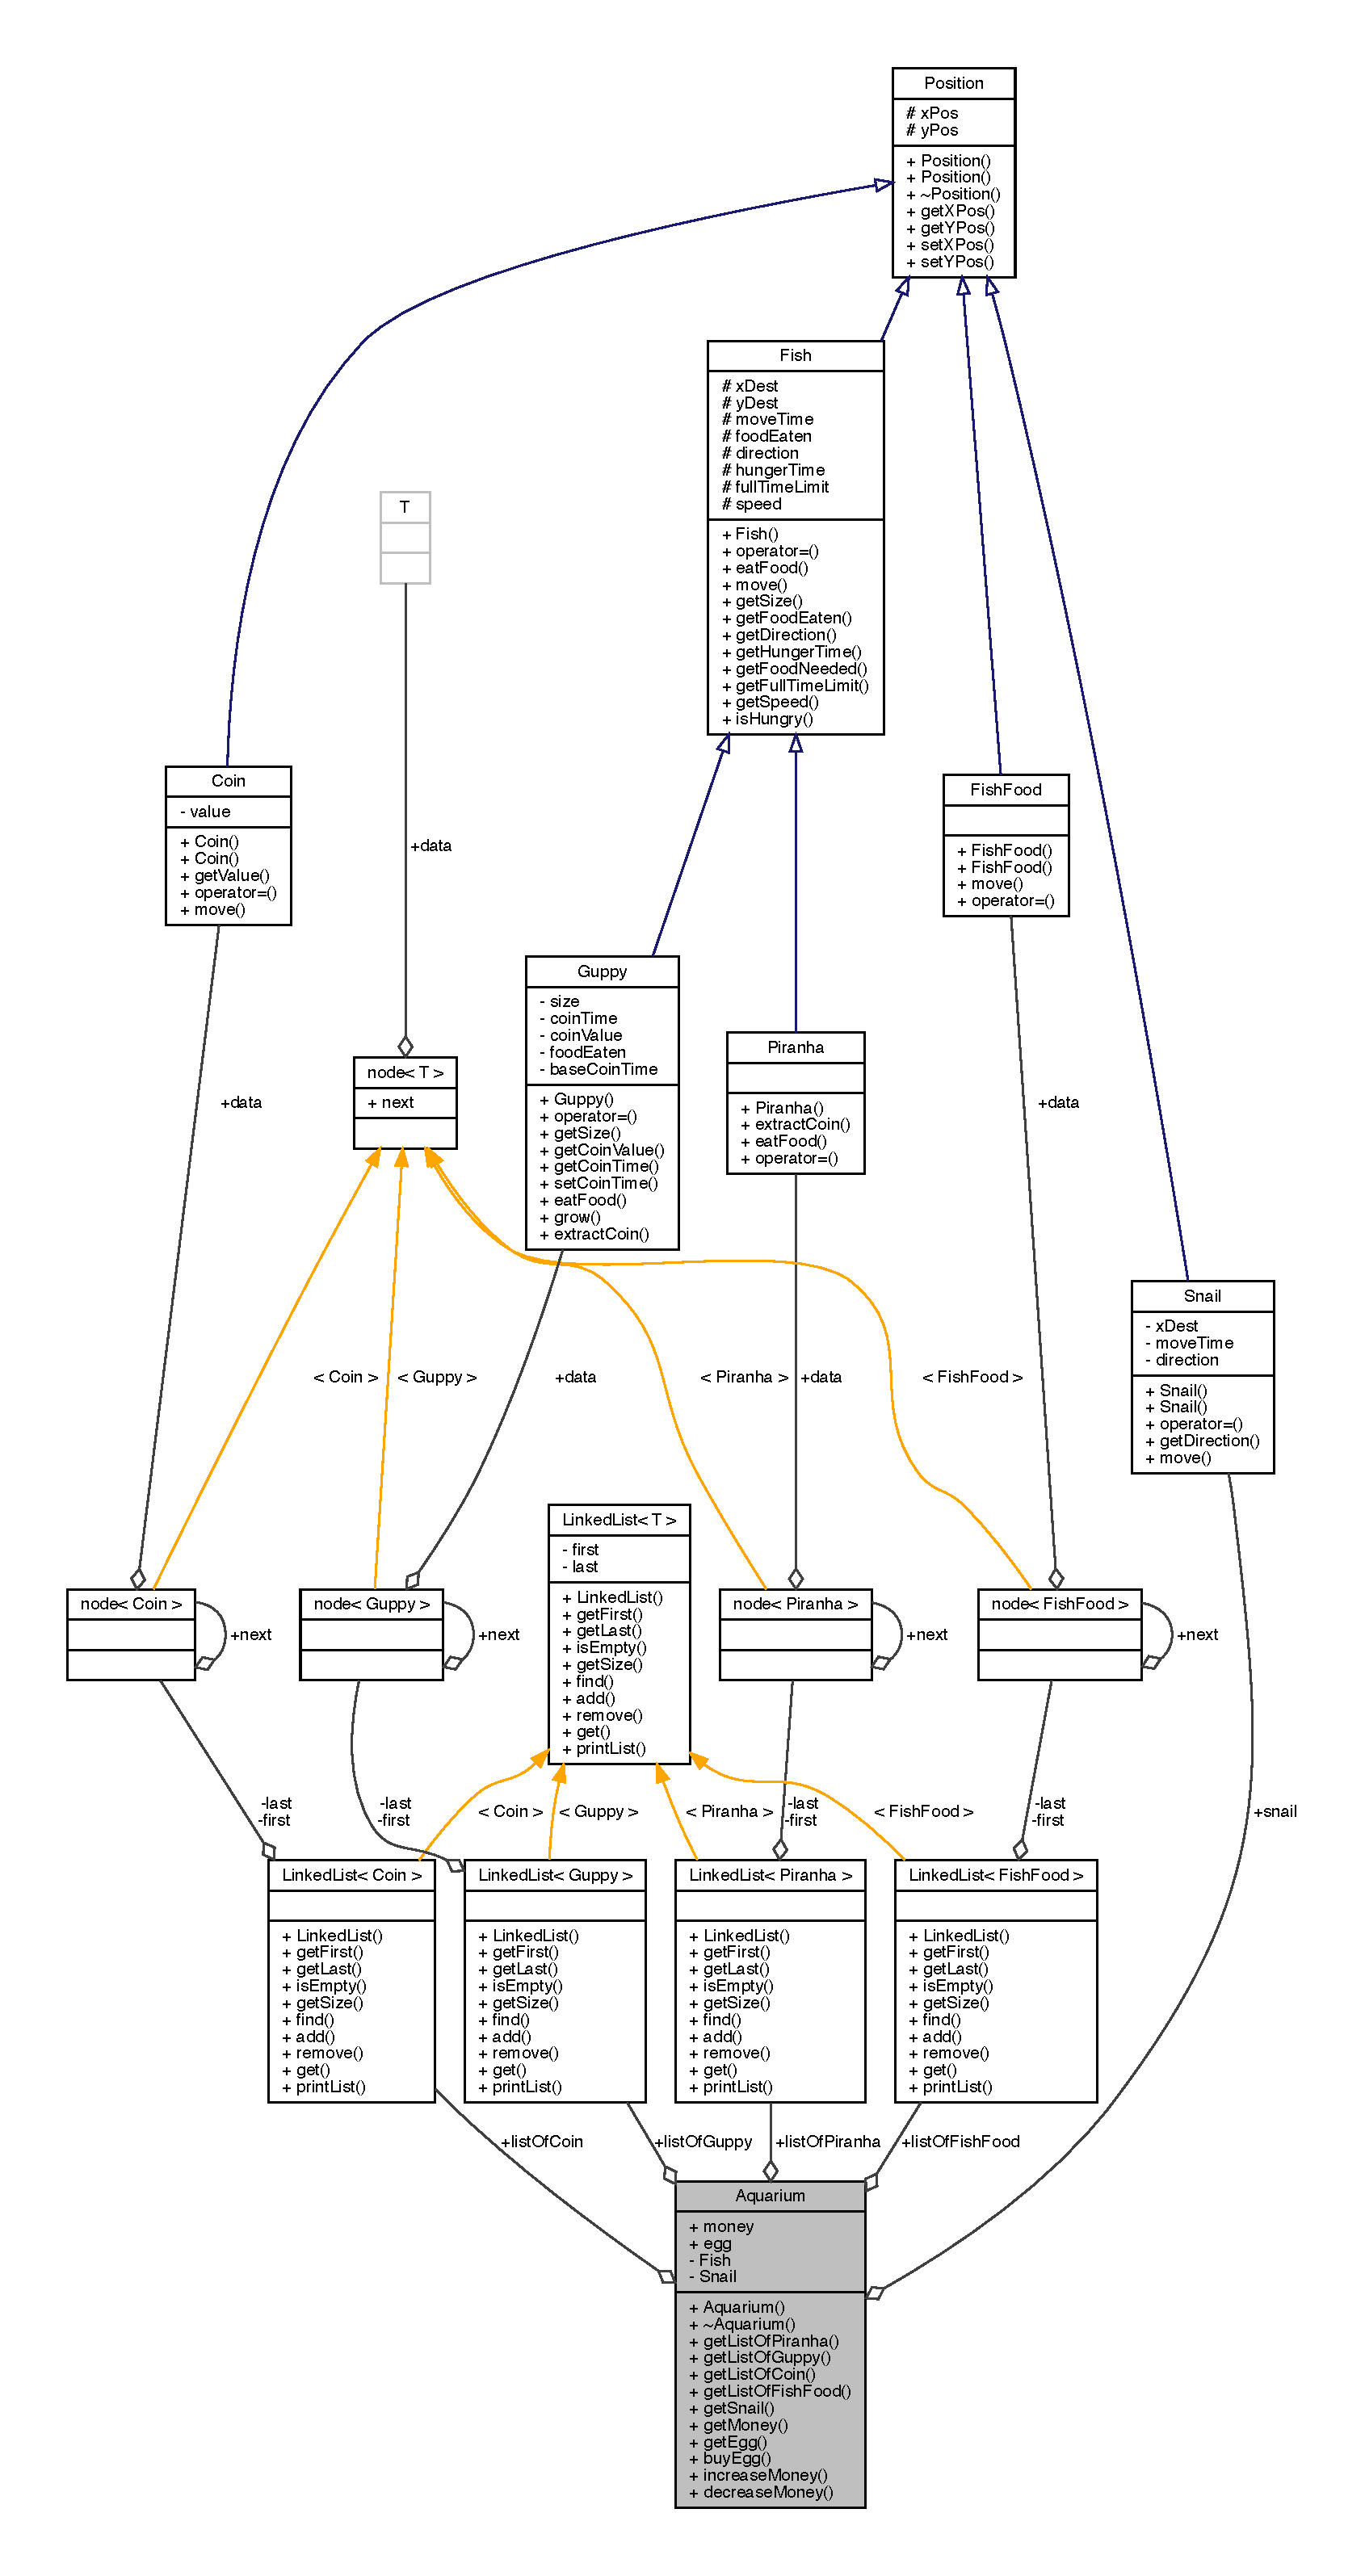
\includegraphics[height=550pt]{class_aquarium__coll__graph}
\end{center}
\end{figure}
\subsection*{Public Member Functions}
\begin{DoxyCompactItemize}
\item 
\mbox{\hyperlink{class_aquarium_a0176cc59bd34e39fd3d79d56d4db4d08}{Aquarium}} ()
\item 
\mbox{\hyperlink{class_aquarium_a40f31f27104d48e4f558d40059f4a590}{$\sim$\+Aquarium}} ()
\item 
\mbox{\hyperlink{class_linked_list}{Linked\+List}}$<$ \mbox{\hyperlink{class_piranha}{Piranha}} $>$ \mbox{\hyperlink{class_aquarium_a3fb338105afbdb86806f721a2bf15dda}{get\+List\+Of\+Piranha}} () const
\item 
\mbox{\hyperlink{class_linked_list}{Linked\+List}}$<$ \mbox{\hyperlink{class_guppy}{Guppy}} $>$ \mbox{\hyperlink{class_aquarium_a745e4d67436255cc4dbb4285d6413eb3}{get\+List\+Of\+Guppy}} () const
\item 
\mbox{\hyperlink{class_linked_list}{Linked\+List}}$<$ \mbox{\hyperlink{class_coin}{Coin}} $>$ \mbox{\hyperlink{class_aquarium_a5d8a7dd4849b12c9fdc3a8a43ab4d4a0}{get\+List\+Of\+Coin}} () const
\item 
\mbox{\hyperlink{class_linked_list}{Linked\+List}}$<$ \mbox{\hyperlink{class_fish_food}{Fish\+Food}} $>$ \mbox{\hyperlink{class_aquarium_a499b9583503fde6e0dbc16a4c73bc706}{get\+List\+Of\+Fish\+Food}} () const
\item 
\mbox{\hyperlink{class_snail}{Snail}} \& \mbox{\hyperlink{class_aquarium_aeba34bc057163d89f62f7ed06fad4075}{get\+Snail}} ()
\item 
int \mbox{\hyperlink{class_aquarium_a7622156e901ca61c60b32ed8f6f5ace9}{get\+Money}} ()
\item 
int \mbox{\hyperlink{class_aquarium_af74c3502752a20b2d2b8832342b243b7}{get\+Egg}} ()
\item 
void \mbox{\hyperlink{class_aquarium_a5e26a35a516d1e6db1e3c4b7f367e498}{buy\+Egg}} ()
\item 
void \mbox{\hyperlink{class_aquarium_a5274f810d3322c4992aae11dbe8d7e87}{increase\+Money}} (int)
\item 
void \mbox{\hyperlink{class_aquarium_a6af7636a999b3d42f2d313d59e9cf88e}{decrease\+Money}} (int)
\end{DoxyCompactItemize}
\subsection*{Public Attributes}
\begin{DoxyCompactItemize}
\item 
\mbox{\hyperlink{class_linked_list}{Linked\+List}}$<$ \mbox{\hyperlink{class_piranha}{Piranha}} $>$ \mbox{\hyperlink{class_aquarium_a5914c6e8860d90a55bb153bd7190c75d}{list\+Of\+Piranha}}
\item 
\mbox{\hyperlink{class_linked_list}{Linked\+List}}$<$ \mbox{\hyperlink{class_guppy}{Guppy}} $>$ \mbox{\hyperlink{class_aquarium_a974abef2727deb91bc52d5b4b5ed93cc}{list\+Of\+Guppy}}
\item 
\mbox{\hyperlink{class_linked_list}{Linked\+List}}$<$ \mbox{\hyperlink{class_coin}{Coin}} $>$ \mbox{\hyperlink{class_aquarium_a81d4d13fb34cb230fb8aeb7c578edd8e}{list\+Of\+Coin}}
\item 
\mbox{\hyperlink{class_linked_list}{Linked\+List}}$<$ \mbox{\hyperlink{class_fish_food}{Fish\+Food}} $>$ \mbox{\hyperlink{class_aquarium_a8792367505556ece7fd7ce0fe63dbf51}{list\+Of\+Fish\+Food}}
\item 
\mbox{\hyperlink{class_snail}{Snail}} \mbox{\hyperlink{class_aquarium_a031f639386ae1f30bda7d97f75781b17}{snail}}
\item 
int \mbox{\hyperlink{class_aquarium_a763165a06487cca929dfe5601a9254cb}{money}}
\item 
int \mbox{\hyperlink{class_aquarium_a4f12b488315834787132112b4de5f186}{egg}}
\end{DoxyCompactItemize}
\subsection*{Private Attributes}
\begin{DoxyCompactItemize}
\item 
friend \mbox{\hyperlink{class_aquarium_ae7f1e47f6e70e618d97f6f6497556bd2}{Fish}}
\item 
friend \mbox{\hyperlink{class_aquarium_af6f4e7e46567d5a7c55c4c6529d81deb}{Snail}}
\end{DoxyCompactItemize}


\subsection{Constructor \& Destructor Documentation}
\mbox{\Hypertarget{class_aquarium_a0176cc59bd34e39fd3d79d56d4db4d08}\label{class_aquarium_a0176cc59bd34e39fd3d79d56d4db4d08}} 
\index{Aquarium@{Aquarium}!Aquarium@{Aquarium}}
\index{Aquarium@{Aquarium}!Aquarium@{Aquarium}}
\subsubsection{\texorpdfstring{Aquarium()}{Aquarium()}}
{\footnotesize\ttfamily Aquarium\+::\+Aquarium (\begin{DoxyParamCaption}{ }\end{DoxyParamCaption})}

Here is the call graph for this function\+:
\nopagebreak
\begin{figure}[H]
\begin{center}
\leavevmode
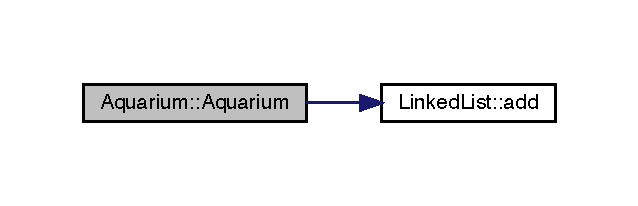
\includegraphics[width=306pt]{class_aquarium_a0176cc59bd34e39fd3d79d56d4db4d08_cgraph}
\end{center}
\end{figure}
\mbox{\Hypertarget{class_aquarium_a40f31f27104d48e4f558d40059f4a590}\label{class_aquarium_a40f31f27104d48e4f558d40059f4a590}} 
\index{Aquarium@{Aquarium}!````~Aquarium@{$\sim$\+Aquarium}}
\index{````~Aquarium@{$\sim$\+Aquarium}!Aquarium@{Aquarium}}
\subsubsection{\texorpdfstring{$\sim$\+Aquarium()}{~Aquarium()}}
{\footnotesize\ttfamily Aquarium\+::$\sim$\+Aquarium (\begin{DoxyParamCaption}{ }\end{DoxyParamCaption})}



\subsection{Member Function Documentation}
\mbox{\Hypertarget{class_aquarium_a5e26a35a516d1e6db1e3c4b7f367e498}\label{class_aquarium_a5e26a35a516d1e6db1e3c4b7f367e498}} 
\index{Aquarium@{Aquarium}!buy\+Egg@{buy\+Egg}}
\index{buy\+Egg@{buy\+Egg}!Aquarium@{Aquarium}}
\subsubsection{\texorpdfstring{buy\+Egg()}{buyEgg()}}
{\footnotesize\ttfamily void Aquarium\+::buy\+Egg (\begin{DoxyParamCaption}{ }\end{DoxyParamCaption})}

\mbox{\Hypertarget{class_aquarium_a6af7636a999b3d42f2d313d59e9cf88e}\label{class_aquarium_a6af7636a999b3d42f2d313d59e9cf88e}} 
\index{Aquarium@{Aquarium}!decrease\+Money@{decrease\+Money}}
\index{decrease\+Money@{decrease\+Money}!Aquarium@{Aquarium}}
\subsubsection{\texorpdfstring{decrease\+Money()}{decreaseMoney()}}
{\footnotesize\ttfamily void Aquarium\+::decrease\+Money (\begin{DoxyParamCaption}\item[{int}]{value }\end{DoxyParamCaption})}

\mbox{\Hypertarget{class_aquarium_af74c3502752a20b2d2b8832342b243b7}\label{class_aquarium_af74c3502752a20b2d2b8832342b243b7}} 
\index{Aquarium@{Aquarium}!get\+Egg@{get\+Egg}}
\index{get\+Egg@{get\+Egg}!Aquarium@{Aquarium}}
\subsubsection{\texorpdfstring{get\+Egg()}{getEgg()}}
{\footnotesize\ttfamily int Aquarium\+::get\+Egg (\begin{DoxyParamCaption}{ }\end{DoxyParamCaption})}

\mbox{\Hypertarget{class_aquarium_a5d8a7dd4849b12c9fdc3a8a43ab4d4a0}\label{class_aquarium_a5d8a7dd4849b12c9fdc3a8a43ab4d4a0}} 
\index{Aquarium@{Aquarium}!get\+List\+Of\+Coin@{get\+List\+Of\+Coin}}
\index{get\+List\+Of\+Coin@{get\+List\+Of\+Coin}!Aquarium@{Aquarium}}
\subsubsection{\texorpdfstring{get\+List\+Of\+Coin()}{getListOfCoin()}}
{\footnotesize\ttfamily \mbox{\hyperlink{class_linked_list}{Linked\+List}}$<$ \mbox{\hyperlink{class_coin}{Coin}} $>$ Aquarium\+::get\+List\+Of\+Coin (\begin{DoxyParamCaption}{ }\end{DoxyParamCaption}) const}

\mbox{\Hypertarget{class_aquarium_a499b9583503fde6e0dbc16a4c73bc706}\label{class_aquarium_a499b9583503fde6e0dbc16a4c73bc706}} 
\index{Aquarium@{Aquarium}!get\+List\+Of\+Fish\+Food@{get\+List\+Of\+Fish\+Food}}
\index{get\+List\+Of\+Fish\+Food@{get\+List\+Of\+Fish\+Food}!Aquarium@{Aquarium}}
\subsubsection{\texorpdfstring{get\+List\+Of\+Fish\+Food()}{getListOfFishFood()}}
{\footnotesize\ttfamily \mbox{\hyperlink{class_linked_list}{Linked\+List}}$<$ \mbox{\hyperlink{class_fish_food}{Fish\+Food}} $>$ Aquarium\+::get\+List\+Of\+Fish\+Food (\begin{DoxyParamCaption}{ }\end{DoxyParamCaption}) const}

\mbox{\Hypertarget{class_aquarium_a745e4d67436255cc4dbb4285d6413eb3}\label{class_aquarium_a745e4d67436255cc4dbb4285d6413eb3}} 
\index{Aquarium@{Aquarium}!get\+List\+Of\+Guppy@{get\+List\+Of\+Guppy}}
\index{get\+List\+Of\+Guppy@{get\+List\+Of\+Guppy}!Aquarium@{Aquarium}}
\subsubsection{\texorpdfstring{get\+List\+Of\+Guppy()}{getListOfGuppy()}}
{\footnotesize\ttfamily \mbox{\hyperlink{class_linked_list}{Linked\+List}}$<$ \mbox{\hyperlink{class_guppy}{Guppy}} $>$ Aquarium\+::get\+List\+Of\+Guppy (\begin{DoxyParamCaption}{ }\end{DoxyParamCaption}) const}

\mbox{\Hypertarget{class_aquarium_a3fb338105afbdb86806f721a2bf15dda}\label{class_aquarium_a3fb338105afbdb86806f721a2bf15dda}} 
\index{Aquarium@{Aquarium}!get\+List\+Of\+Piranha@{get\+List\+Of\+Piranha}}
\index{get\+List\+Of\+Piranha@{get\+List\+Of\+Piranha}!Aquarium@{Aquarium}}
\subsubsection{\texorpdfstring{get\+List\+Of\+Piranha()}{getListOfPiranha()}}
{\footnotesize\ttfamily \mbox{\hyperlink{class_linked_list}{Linked\+List}}$<$ \mbox{\hyperlink{class_piranha}{Piranha}} $>$ Aquarium\+::get\+List\+Of\+Piranha (\begin{DoxyParamCaption}{ }\end{DoxyParamCaption}) const}

\mbox{\Hypertarget{class_aquarium_a7622156e901ca61c60b32ed8f6f5ace9}\label{class_aquarium_a7622156e901ca61c60b32ed8f6f5ace9}} 
\index{Aquarium@{Aquarium}!get\+Money@{get\+Money}}
\index{get\+Money@{get\+Money}!Aquarium@{Aquarium}}
\subsubsection{\texorpdfstring{get\+Money()}{getMoney()}}
{\footnotesize\ttfamily int Aquarium\+::get\+Money (\begin{DoxyParamCaption}{ }\end{DoxyParamCaption})}

\mbox{\Hypertarget{class_aquarium_aeba34bc057163d89f62f7ed06fad4075}\label{class_aquarium_aeba34bc057163d89f62f7ed06fad4075}} 
\index{Aquarium@{Aquarium}!get\+Snail@{get\+Snail}}
\index{get\+Snail@{get\+Snail}!Aquarium@{Aquarium}}
\subsubsection{\texorpdfstring{get\+Snail()}{getSnail()}}
{\footnotesize\ttfamily \mbox{\hyperlink{class_snail}{Snail}} \& Aquarium\+::get\+Snail (\begin{DoxyParamCaption}{ }\end{DoxyParamCaption})}

\mbox{\Hypertarget{class_aquarium_a5274f810d3322c4992aae11dbe8d7e87}\label{class_aquarium_a5274f810d3322c4992aae11dbe8d7e87}} 
\index{Aquarium@{Aquarium}!increase\+Money@{increase\+Money}}
\index{increase\+Money@{increase\+Money}!Aquarium@{Aquarium}}
\subsubsection{\texorpdfstring{increase\+Money()}{increaseMoney()}}
{\footnotesize\ttfamily void Aquarium\+::increase\+Money (\begin{DoxyParamCaption}\item[{int}]{value }\end{DoxyParamCaption})}



\subsection{Member Data Documentation}
\mbox{\Hypertarget{class_aquarium_a4f12b488315834787132112b4de5f186}\label{class_aquarium_a4f12b488315834787132112b4de5f186}} 
\index{Aquarium@{Aquarium}!egg@{egg}}
\index{egg@{egg}!Aquarium@{Aquarium}}
\subsubsection{\texorpdfstring{egg}{egg}}
{\footnotesize\ttfamily int Aquarium\+::egg}

\mbox{\Hypertarget{class_aquarium_ae7f1e47f6e70e618d97f6f6497556bd2}\label{class_aquarium_ae7f1e47f6e70e618d97f6f6497556bd2}} 
\index{Aquarium@{Aquarium}!Fish@{Fish}}
\index{Fish@{Fish}!Aquarium@{Aquarium}}
\subsubsection{\texorpdfstring{Fish}{Fish}}
{\footnotesize\ttfamily friend Aquarium\+::\+Fish\hspace{0.3cm}{\ttfamily [private]}}

\mbox{\Hypertarget{class_aquarium_a81d4d13fb34cb230fb8aeb7c578edd8e}\label{class_aquarium_a81d4d13fb34cb230fb8aeb7c578edd8e}} 
\index{Aquarium@{Aquarium}!list\+Of\+Coin@{list\+Of\+Coin}}
\index{list\+Of\+Coin@{list\+Of\+Coin}!Aquarium@{Aquarium}}
\subsubsection{\texorpdfstring{list\+Of\+Coin}{listOfCoin}}
{\footnotesize\ttfamily \mbox{\hyperlink{class_linked_list}{Linked\+List}}$<$\mbox{\hyperlink{class_coin}{Coin}}$>$ Aquarium\+::list\+Of\+Coin}

\mbox{\Hypertarget{class_aquarium_a8792367505556ece7fd7ce0fe63dbf51}\label{class_aquarium_a8792367505556ece7fd7ce0fe63dbf51}} 
\index{Aquarium@{Aquarium}!list\+Of\+Fish\+Food@{list\+Of\+Fish\+Food}}
\index{list\+Of\+Fish\+Food@{list\+Of\+Fish\+Food}!Aquarium@{Aquarium}}
\subsubsection{\texorpdfstring{list\+Of\+Fish\+Food}{listOfFishFood}}
{\footnotesize\ttfamily \mbox{\hyperlink{class_linked_list}{Linked\+List}}$<$\mbox{\hyperlink{class_fish_food}{Fish\+Food}}$>$ Aquarium\+::list\+Of\+Fish\+Food}

\mbox{\Hypertarget{class_aquarium_a974abef2727deb91bc52d5b4b5ed93cc}\label{class_aquarium_a974abef2727deb91bc52d5b4b5ed93cc}} 
\index{Aquarium@{Aquarium}!list\+Of\+Guppy@{list\+Of\+Guppy}}
\index{list\+Of\+Guppy@{list\+Of\+Guppy}!Aquarium@{Aquarium}}
\subsubsection{\texorpdfstring{list\+Of\+Guppy}{listOfGuppy}}
{\footnotesize\ttfamily \mbox{\hyperlink{class_linked_list}{Linked\+List}}$<$\mbox{\hyperlink{class_guppy}{Guppy}}$>$ Aquarium\+::list\+Of\+Guppy}

\mbox{\Hypertarget{class_aquarium_a5914c6e8860d90a55bb153bd7190c75d}\label{class_aquarium_a5914c6e8860d90a55bb153bd7190c75d}} 
\index{Aquarium@{Aquarium}!list\+Of\+Piranha@{list\+Of\+Piranha}}
\index{list\+Of\+Piranha@{list\+Of\+Piranha}!Aquarium@{Aquarium}}
\subsubsection{\texorpdfstring{list\+Of\+Piranha}{listOfPiranha}}
{\footnotesize\ttfamily \mbox{\hyperlink{class_linked_list}{Linked\+List}}$<$\mbox{\hyperlink{class_piranha}{Piranha}}$>$ Aquarium\+::list\+Of\+Piranha}

\mbox{\Hypertarget{class_aquarium_a763165a06487cca929dfe5601a9254cb}\label{class_aquarium_a763165a06487cca929dfe5601a9254cb}} 
\index{Aquarium@{Aquarium}!money@{money}}
\index{money@{money}!Aquarium@{Aquarium}}
\subsubsection{\texorpdfstring{money}{money}}
{\footnotesize\ttfamily int Aquarium\+::money}

\mbox{\Hypertarget{class_aquarium_af6f4e7e46567d5a7c55c4c6529d81deb}\label{class_aquarium_af6f4e7e46567d5a7c55c4c6529d81deb}} 
\index{Aquarium@{Aquarium}!Snail@{Snail}}
\index{Snail@{Snail}!Aquarium@{Aquarium}}
\subsubsection{\texorpdfstring{Snail}{Snail}}
{\footnotesize\ttfamily friend Aquarium\+::\+Snail\hspace{0.3cm}{\ttfamily [private]}}

\mbox{\Hypertarget{class_aquarium_a031f639386ae1f30bda7d97f75781b17}\label{class_aquarium_a031f639386ae1f30bda7d97f75781b17}} 
\index{Aquarium@{Aquarium}!snail@{snail}}
\index{snail@{snail}!Aquarium@{Aquarium}}
\subsubsection{\texorpdfstring{snail}{snail}}
{\footnotesize\ttfamily \mbox{\hyperlink{class_snail}{Snail}} Aquarium\+::snail}



The documentation for this class was generated from the following files\+:\begin{DoxyCompactItemize}
\item 
\mbox{\hyperlink{_aquarium_8hpp}{Aquarium.\+hpp}}\item 
\mbox{\hyperlink{_aquarium_8cpp}{Aquarium.\+cpp}}\end{DoxyCompactItemize}

\hypertarget{class_coin}{}\section{Coin Class Reference}
\label{class_coin}\index{Coin@{Coin}}


{\ttfamily \#include $<$Coin.\+hpp$>$}



Inheritance diagram for Coin\+:
\nopagebreak
\begin{figure}[H]
\begin{center}
\leavevmode
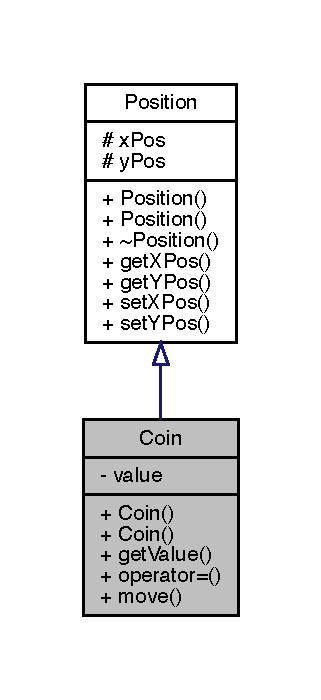
\includegraphics[width=154pt]{class_coin__inherit__graph}
\end{center}
\end{figure}


Collaboration diagram for Coin\+:
\nopagebreak
\begin{figure}[H]
\begin{center}
\leavevmode
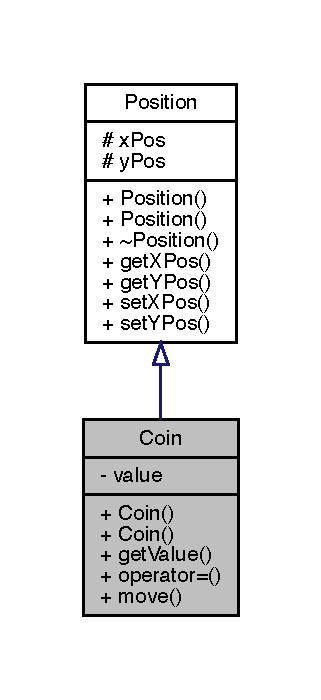
\includegraphics[width=154pt]{class_coin__coll__graph}
\end{center}
\end{figure}
\subsection*{Public Member Functions}
\begin{DoxyCompactItemize}
\item 
\mbox{\hyperlink{class_coin_a94b2130e2d3ac956ba47271ad81c64f5}{Coin}} ()
\item 
\mbox{\hyperlink{class_coin_ad9c43b40a4d31b251225e44cac231679}{Coin}} (double, double, double)
\item 
double \mbox{\hyperlink{class_coin_a53cbddb74ac97ec54ec40f09beab3332}{get\+Value}} () const
\item 
\mbox{\hyperlink{class_coin}{Coin}} \mbox{\hyperlink{class_coin_adaf4dcbe15a8d4549b4ccdaaca18c9bb}{operator=}} (const \mbox{\hyperlink{class_coin}{Coin}} \&C)
\item 
void \mbox{\hyperlink{class_coin_a58a2a28aa6c21f0045983755dad015dc}{move}} (double t)
\end{DoxyCompactItemize}
\subsection*{Private Attributes}
\begin{DoxyCompactItemize}
\item 
double \mbox{\hyperlink{class_coin_ada7dce9fece24cd203828ec6399b7a86}{value}}
\end{DoxyCompactItemize}
\subsection*{Additional Inherited Members}


\subsection{Constructor \& Destructor Documentation}
\mbox{\Hypertarget{class_coin_a94b2130e2d3ac956ba47271ad81c64f5}\label{class_coin_a94b2130e2d3ac956ba47271ad81c64f5}} 
\index{Coin@{Coin}!Coin@{Coin}}
\index{Coin@{Coin}!Coin@{Coin}}
\subsubsection{\texorpdfstring{Coin()}{Coin()}\hspace{0.1cm}{\footnotesize\ttfamily [1/2]}}
{\footnotesize\ttfamily Coin\+::\+Coin (\begin{DoxyParamCaption}{ }\end{DoxyParamCaption})}

\mbox{\Hypertarget{class_coin_ad9c43b40a4d31b251225e44cac231679}\label{class_coin_ad9c43b40a4d31b251225e44cac231679}} 
\index{Coin@{Coin}!Coin@{Coin}}
\index{Coin@{Coin}!Coin@{Coin}}
\subsubsection{\texorpdfstring{Coin()}{Coin()}\hspace{0.1cm}{\footnotesize\ttfamily [2/2]}}
{\footnotesize\ttfamily Coin\+::\+Coin (\begin{DoxyParamCaption}\item[{double}]{\+\_\+value,  }\item[{double}]{\+\_\+xpos,  }\item[{double}]{\+\_\+ypos }\end{DoxyParamCaption})}



\subsection{Member Function Documentation}
\mbox{\Hypertarget{class_coin_a53cbddb74ac97ec54ec40f09beab3332}\label{class_coin_a53cbddb74ac97ec54ec40f09beab3332}} 
\index{Coin@{Coin}!get\+Value@{get\+Value}}
\index{get\+Value@{get\+Value}!Coin@{Coin}}
\subsubsection{\texorpdfstring{get\+Value()}{getValue()}}
{\footnotesize\ttfamily double Coin\+::get\+Value (\begin{DoxyParamCaption}{ }\end{DoxyParamCaption}) const}

\mbox{\Hypertarget{class_coin_a58a2a28aa6c21f0045983755dad015dc}\label{class_coin_a58a2a28aa6c21f0045983755dad015dc}} 
\index{Coin@{Coin}!move@{move}}
\index{move@{move}!Coin@{Coin}}
\subsubsection{\texorpdfstring{move()}{move()}}
{\footnotesize\ttfamily void Coin\+::move (\begin{DoxyParamCaption}\item[{double}]{t }\end{DoxyParamCaption})}

\mbox{\Hypertarget{class_coin_adaf4dcbe15a8d4549b4ccdaaca18c9bb}\label{class_coin_adaf4dcbe15a8d4549b4ccdaaca18c9bb}} 
\index{Coin@{Coin}!operator=@{operator=}}
\index{operator=@{operator=}!Coin@{Coin}}
\subsubsection{\texorpdfstring{operator=()}{operator=()}}
{\footnotesize\ttfamily \mbox{\hyperlink{class_coin}{Coin}} Coin\+::operator= (\begin{DoxyParamCaption}\item[{const \mbox{\hyperlink{class_coin}{Coin}} \&}]{C }\end{DoxyParamCaption})}

Here is the call graph for this function\+:
\nopagebreak
\begin{figure}[H]
\begin{center}
\leavevmode
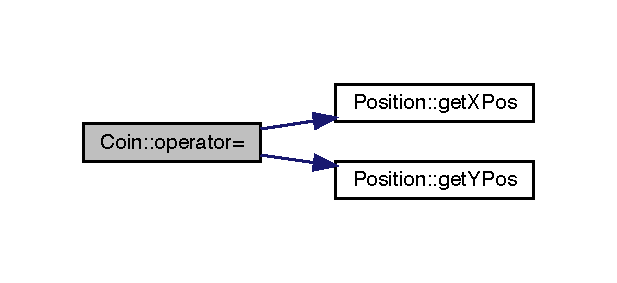
\includegraphics[width=296pt]{class_coin_adaf4dcbe15a8d4549b4ccdaaca18c9bb_cgraph}
\end{center}
\end{figure}


\subsection{Member Data Documentation}
\mbox{\Hypertarget{class_coin_ada7dce9fece24cd203828ec6399b7a86}\label{class_coin_ada7dce9fece24cd203828ec6399b7a86}} 
\index{Coin@{Coin}!value@{value}}
\index{value@{value}!Coin@{Coin}}
\subsubsection{\texorpdfstring{value}{value}}
{\footnotesize\ttfamily double Coin\+::value\hspace{0.3cm}{\ttfamily [private]}}



The documentation for this class was generated from the following files\+:\begin{DoxyCompactItemize}
\item 
\mbox{\hyperlink{_coin_8hpp}{Coin.\+hpp}}\item 
\mbox{\hyperlink{_coin_8cpp}{Coin.\+cpp}}\end{DoxyCompactItemize}

\hypertarget{class_fish}{}\section{Fish Class Reference}
\label{class_fish}\index{Fish@{Fish}}


{\ttfamily \#include $<$Fish.\+hpp$>$}



Inheritance diagram for Fish\+:
\nopagebreak
\begin{figure}[H]
\begin{center}
\leavevmode
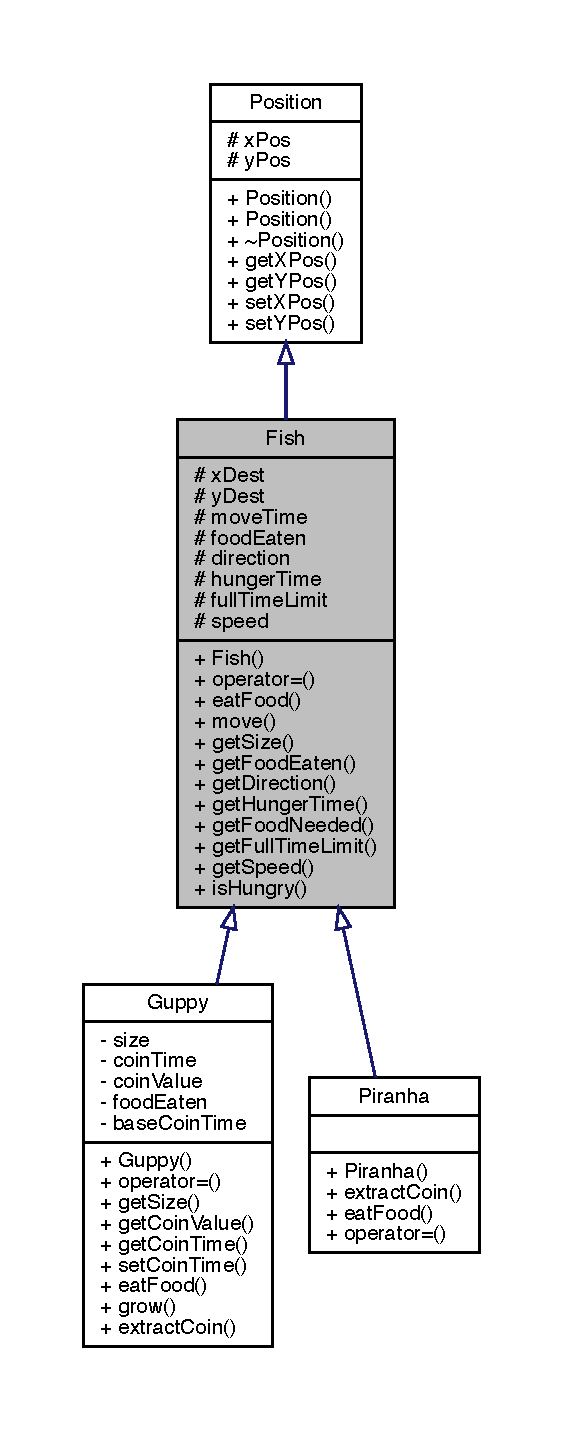
\includegraphics[height=550pt]{class_fish__inherit__graph}
\end{center}
\end{figure}


Collaboration diagram for Fish\+:
\nopagebreak
\begin{figure}[H]
\begin{center}
\leavevmode
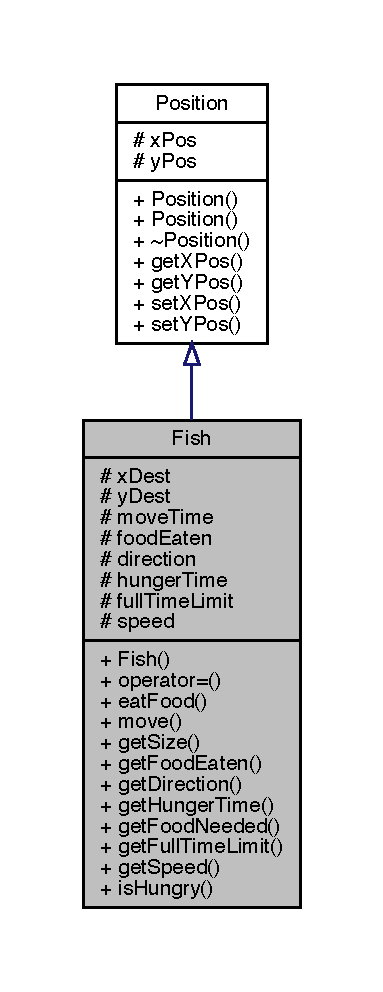
\includegraphics[width=184pt]{class_fish__coll__graph}
\end{center}
\end{figure}
\subsection*{Public Member Functions}
\begin{DoxyCompactItemize}
\item 
\mbox{\hyperlink{class_fish_a265fa9dc23037b5f621ff5f2b2731e9b}{Fish}} ()
\item 
\mbox{\hyperlink{class_fish}{Fish}} \& \mbox{\hyperlink{class_fish_a45789c6c8ecafbcfae866845f34a7f33}{operator=}} (const \mbox{\hyperlink{class_fish}{Fish}} \&F)
\item 
virtual void \mbox{\hyperlink{class_fish_aad629fb35c786b2a44c1204d011f9ae4}{eat\+Food}} ()=0
\item 
void \mbox{\hyperlink{class_fish_ae746baf504f478e83b7b314b7e80eb48}{move}} (double, double, double, bool)
\item 
int \mbox{\hyperlink{class_fish_a00b7df960ce799914b15b0e95ecfa4c8}{get\+Size}} () const
\item 
int \mbox{\hyperlink{class_fish_a43f71b5e1940fec9aee01ba7ecb7cc5b}{get\+Food\+Eaten}} () const
\item 
bool \mbox{\hyperlink{class_fish_a411294175d2104ba12bf205b529f59bd}{get\+Direction}} () const
\item 
int \mbox{\hyperlink{class_fish_aca713642313f9c438e900235c0c727d6}{get\+Hunger\+Time}} () const
\item 
int \mbox{\hyperlink{class_fish_a5ebfe16e94d3e605d703efbd47aa2a07}{get\+Food\+Needed}} () const
\item 
int \mbox{\hyperlink{class_fish_a40a7508eeee947749bc76e67eeca01cc}{get\+Full\+Time\+Limit}} () const
\item 
int \mbox{\hyperlink{class_fish_af495566d33b8e3b83605a8222bc02783}{get\+Speed}} () const
\item 
bool \mbox{\hyperlink{class_fish_a0b45770c92baa9471ae6dc2ebf15d159}{is\+Hungry}} () const
\end{DoxyCompactItemize}
\subsection*{Protected Attributes}
\begin{DoxyCompactItemize}
\item 
double \mbox{\hyperlink{class_fish_a8016badef0a39101994d62825dc69504}{x\+Dest}}
\item 
double \mbox{\hyperlink{class_fish_a27b5905734d7d9f8f3a87fca6fbe2018}{y\+Dest}}
\item 
double \mbox{\hyperlink{class_fish_a44bb72a7856095a8fc17f59b45602bad}{move\+Time}}
\item 
int \mbox{\hyperlink{class_fish_aff94d90077eb91db9f32c518b1dda1aa}{food\+Eaten}}
\item 
bool \mbox{\hyperlink{class_fish_aad304102219bdb3d333df50d8a74fd9d}{direction}}
\item 
int \mbox{\hyperlink{class_fish_a3fc20ca5c769db904d67492f578ecd9a}{hunger\+Time}}
\item 
const int \mbox{\hyperlink{class_fish_aaeccf31f823eb7319bb5201dbf05174a}{full\+Time\+Limit}} = 40
\item 
const int \mbox{\hyperlink{class_fish_a2f84c2eeb84451bc55156ae9da753cc9}{speed}} = 40
\end{DoxyCompactItemize}


\subsection{Constructor \& Destructor Documentation}
\mbox{\Hypertarget{class_fish_a265fa9dc23037b5f621ff5f2b2731e9b}\label{class_fish_a265fa9dc23037b5f621ff5f2b2731e9b}} 
\index{Fish@{Fish}!Fish@{Fish}}
\index{Fish@{Fish}!Fish@{Fish}}
\subsubsection{\texorpdfstring{Fish()}{Fish()}}
{\footnotesize\ttfamily Fish\+::\+Fish (\begin{DoxyParamCaption}{ }\end{DoxyParamCaption})}



\subsection{Member Function Documentation}
\mbox{\Hypertarget{class_fish_aad629fb35c786b2a44c1204d011f9ae4}\label{class_fish_aad629fb35c786b2a44c1204d011f9ae4}} 
\index{Fish@{Fish}!eat\+Food@{eat\+Food}}
\index{eat\+Food@{eat\+Food}!Fish@{Fish}}
\subsubsection{\texorpdfstring{eat\+Food()}{eatFood()}}
{\footnotesize\ttfamily virtual void Fish\+::eat\+Food (\begin{DoxyParamCaption}{ }\end{DoxyParamCaption})\hspace{0.3cm}{\ttfamily [pure virtual]}}



Implemented in \mbox{\hyperlink{class_guppy_a50115297f5c2f4df46e3613e09db115e}{Guppy}}, and \mbox{\hyperlink{class_piranha_a50992b83e072f8719150d302469a462f}{Piranha}}.

\mbox{\Hypertarget{class_fish_a411294175d2104ba12bf205b529f59bd}\label{class_fish_a411294175d2104ba12bf205b529f59bd}} 
\index{Fish@{Fish}!get\+Direction@{get\+Direction}}
\index{get\+Direction@{get\+Direction}!Fish@{Fish}}
\subsubsection{\texorpdfstring{get\+Direction()}{getDirection()}}
{\footnotesize\ttfamily bool Fish\+::get\+Direction (\begin{DoxyParamCaption}{ }\end{DoxyParamCaption}) const}

\mbox{\Hypertarget{class_fish_a43f71b5e1940fec9aee01ba7ecb7cc5b}\label{class_fish_a43f71b5e1940fec9aee01ba7ecb7cc5b}} 
\index{Fish@{Fish}!get\+Food\+Eaten@{get\+Food\+Eaten}}
\index{get\+Food\+Eaten@{get\+Food\+Eaten}!Fish@{Fish}}
\subsubsection{\texorpdfstring{get\+Food\+Eaten()}{getFoodEaten()}}
{\footnotesize\ttfamily int Fish\+::get\+Food\+Eaten (\begin{DoxyParamCaption}{ }\end{DoxyParamCaption}) const}

\mbox{\Hypertarget{class_fish_a5ebfe16e94d3e605d703efbd47aa2a07}\label{class_fish_a5ebfe16e94d3e605d703efbd47aa2a07}} 
\index{Fish@{Fish}!get\+Food\+Needed@{get\+Food\+Needed}}
\index{get\+Food\+Needed@{get\+Food\+Needed}!Fish@{Fish}}
\subsubsection{\texorpdfstring{get\+Food\+Needed()}{getFoodNeeded()}}
{\footnotesize\ttfamily int Fish\+::get\+Food\+Needed (\begin{DoxyParamCaption}{ }\end{DoxyParamCaption}) const}

\mbox{\Hypertarget{class_fish_a40a7508eeee947749bc76e67eeca01cc}\label{class_fish_a40a7508eeee947749bc76e67eeca01cc}} 
\index{Fish@{Fish}!get\+Full\+Time\+Limit@{get\+Full\+Time\+Limit}}
\index{get\+Full\+Time\+Limit@{get\+Full\+Time\+Limit}!Fish@{Fish}}
\subsubsection{\texorpdfstring{get\+Full\+Time\+Limit()}{getFullTimeLimit()}}
{\footnotesize\ttfamily int Fish\+::get\+Full\+Time\+Limit (\begin{DoxyParamCaption}{ }\end{DoxyParamCaption}) const}

\mbox{\Hypertarget{class_fish_aca713642313f9c438e900235c0c727d6}\label{class_fish_aca713642313f9c438e900235c0c727d6}} 
\index{Fish@{Fish}!get\+Hunger\+Time@{get\+Hunger\+Time}}
\index{get\+Hunger\+Time@{get\+Hunger\+Time}!Fish@{Fish}}
\subsubsection{\texorpdfstring{get\+Hunger\+Time()}{getHungerTime()}}
{\footnotesize\ttfamily int Fish\+::get\+Hunger\+Time (\begin{DoxyParamCaption}{ }\end{DoxyParamCaption}) const}

\mbox{\Hypertarget{class_fish_a00b7df960ce799914b15b0e95ecfa4c8}\label{class_fish_a00b7df960ce799914b15b0e95ecfa4c8}} 
\index{Fish@{Fish}!get\+Size@{get\+Size}}
\index{get\+Size@{get\+Size}!Fish@{Fish}}
\subsubsection{\texorpdfstring{get\+Size()}{getSize()}}
{\footnotesize\ttfamily int Fish\+::get\+Size (\begin{DoxyParamCaption}{ }\end{DoxyParamCaption}) const}

\mbox{\Hypertarget{class_fish_af495566d33b8e3b83605a8222bc02783}\label{class_fish_af495566d33b8e3b83605a8222bc02783}} 
\index{Fish@{Fish}!get\+Speed@{get\+Speed}}
\index{get\+Speed@{get\+Speed}!Fish@{Fish}}
\subsubsection{\texorpdfstring{get\+Speed()}{getSpeed()}}
{\footnotesize\ttfamily int Fish\+::get\+Speed (\begin{DoxyParamCaption}{ }\end{DoxyParamCaption}) const}

\mbox{\Hypertarget{class_fish_a0b45770c92baa9471ae6dc2ebf15d159}\label{class_fish_a0b45770c92baa9471ae6dc2ebf15d159}} 
\index{Fish@{Fish}!is\+Hungry@{is\+Hungry}}
\index{is\+Hungry@{is\+Hungry}!Fish@{Fish}}
\subsubsection{\texorpdfstring{is\+Hungry()}{isHungry()}}
{\footnotesize\ttfamily bool Fish\+::is\+Hungry (\begin{DoxyParamCaption}{ }\end{DoxyParamCaption}) const}

\mbox{\Hypertarget{class_fish_ae746baf504f478e83b7b314b7e80eb48}\label{class_fish_ae746baf504f478e83b7b314b7e80eb48}} 
\index{Fish@{Fish}!move@{move}}
\index{move@{move}!Fish@{Fish}}
\subsubsection{\texorpdfstring{move()}{move()}}
{\footnotesize\ttfamily void Fish\+::move (\begin{DoxyParamCaption}\item[{double}]{x,  }\item[{double}]{y,  }\item[{double}]{t,  }\item[{bool}]{hunt\+Food }\end{DoxyParamCaption})}

\mbox{\Hypertarget{class_fish_a45789c6c8ecafbcfae866845f34a7f33}\label{class_fish_a45789c6c8ecafbcfae866845f34a7f33}} 
\index{Fish@{Fish}!operator=@{operator=}}
\index{operator=@{operator=}!Fish@{Fish}}
\subsubsection{\texorpdfstring{operator=()}{operator=()}}
{\footnotesize\ttfamily \mbox{\hyperlink{class_fish}{Fish}} \& Fish\+::operator= (\begin{DoxyParamCaption}\item[{const \mbox{\hyperlink{class_fish}{Fish}} \&}]{F }\end{DoxyParamCaption})}

Here is the call graph for this function\+:
\nopagebreak
\begin{figure}[H]
\begin{center}
\leavevmode
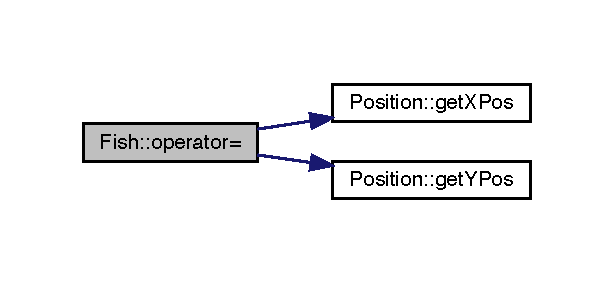
\includegraphics[width=294pt]{class_fish_a45789c6c8ecafbcfae866845f34a7f33_cgraph}
\end{center}
\end{figure}


\subsection{Member Data Documentation}
\mbox{\Hypertarget{class_fish_aad304102219bdb3d333df50d8a74fd9d}\label{class_fish_aad304102219bdb3d333df50d8a74fd9d}} 
\index{Fish@{Fish}!direction@{direction}}
\index{direction@{direction}!Fish@{Fish}}
\subsubsection{\texorpdfstring{direction}{direction}}
{\footnotesize\ttfamily bool Fish\+::direction\hspace{0.3cm}{\ttfamily [protected]}}

\mbox{\Hypertarget{class_fish_aff94d90077eb91db9f32c518b1dda1aa}\label{class_fish_aff94d90077eb91db9f32c518b1dda1aa}} 
\index{Fish@{Fish}!food\+Eaten@{food\+Eaten}}
\index{food\+Eaten@{food\+Eaten}!Fish@{Fish}}
\subsubsection{\texorpdfstring{food\+Eaten}{foodEaten}}
{\footnotesize\ttfamily int Fish\+::food\+Eaten\hspace{0.3cm}{\ttfamily [protected]}}

\mbox{\Hypertarget{class_fish_aaeccf31f823eb7319bb5201dbf05174a}\label{class_fish_aaeccf31f823eb7319bb5201dbf05174a}} 
\index{Fish@{Fish}!full\+Time\+Limit@{full\+Time\+Limit}}
\index{full\+Time\+Limit@{full\+Time\+Limit}!Fish@{Fish}}
\subsubsection{\texorpdfstring{full\+Time\+Limit}{fullTimeLimit}}
{\footnotesize\ttfamily const int Fish\+::full\+Time\+Limit = 40\hspace{0.3cm}{\ttfamily [protected]}}

\mbox{\Hypertarget{class_fish_a3fc20ca5c769db904d67492f578ecd9a}\label{class_fish_a3fc20ca5c769db904d67492f578ecd9a}} 
\index{Fish@{Fish}!hunger\+Time@{hunger\+Time}}
\index{hunger\+Time@{hunger\+Time}!Fish@{Fish}}
\subsubsection{\texorpdfstring{hunger\+Time}{hungerTime}}
{\footnotesize\ttfamily int Fish\+::hunger\+Time\hspace{0.3cm}{\ttfamily [protected]}}

\mbox{\Hypertarget{class_fish_a44bb72a7856095a8fc17f59b45602bad}\label{class_fish_a44bb72a7856095a8fc17f59b45602bad}} 
\index{Fish@{Fish}!move\+Time@{move\+Time}}
\index{move\+Time@{move\+Time}!Fish@{Fish}}
\subsubsection{\texorpdfstring{move\+Time}{moveTime}}
{\footnotesize\ttfamily double Fish\+::move\+Time\hspace{0.3cm}{\ttfamily [protected]}}

\mbox{\Hypertarget{class_fish_a2f84c2eeb84451bc55156ae9da753cc9}\label{class_fish_a2f84c2eeb84451bc55156ae9da753cc9}} 
\index{Fish@{Fish}!speed@{speed}}
\index{speed@{speed}!Fish@{Fish}}
\subsubsection{\texorpdfstring{speed}{speed}}
{\footnotesize\ttfamily const int Fish\+::speed = 40\hspace{0.3cm}{\ttfamily [protected]}}

\mbox{\Hypertarget{class_fish_a8016badef0a39101994d62825dc69504}\label{class_fish_a8016badef0a39101994d62825dc69504}} 
\index{Fish@{Fish}!x\+Dest@{x\+Dest}}
\index{x\+Dest@{x\+Dest}!Fish@{Fish}}
\subsubsection{\texorpdfstring{x\+Dest}{xDest}}
{\footnotesize\ttfamily double Fish\+::x\+Dest\hspace{0.3cm}{\ttfamily [protected]}}

\mbox{\Hypertarget{class_fish_a27b5905734d7d9f8f3a87fca6fbe2018}\label{class_fish_a27b5905734d7d9f8f3a87fca6fbe2018}} 
\index{Fish@{Fish}!y\+Dest@{y\+Dest}}
\index{y\+Dest@{y\+Dest}!Fish@{Fish}}
\subsubsection{\texorpdfstring{y\+Dest}{yDest}}
{\footnotesize\ttfamily double Fish\+::y\+Dest\hspace{0.3cm}{\ttfamily [protected]}}



The documentation for this class was generated from the following files\+:\begin{DoxyCompactItemize}
\item 
\mbox{\hyperlink{_fish_8hpp}{Fish.\+hpp}}\item 
\mbox{\hyperlink{_fish_8cpp}{Fish.\+cpp}}\end{DoxyCompactItemize}

\hypertarget{class_fish_food}{}\section{Fish\+Food Class Reference}
\label{class_fish_food}\index{Fish\+Food@{Fish\+Food}}


{\ttfamily \#include $<$Fish\+Food.\+hpp$>$}



Inheritance diagram for Fish\+Food\+:
\nopagebreak
\begin{figure}[H]
\begin{center}
\leavevmode
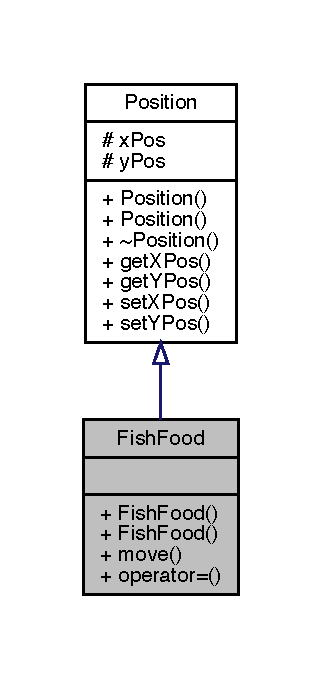
\includegraphics[width=154pt]{class_fish_food__inherit__graph}
\end{center}
\end{figure}


Collaboration diagram for Fish\+Food\+:
\nopagebreak
\begin{figure}[H]
\begin{center}
\leavevmode
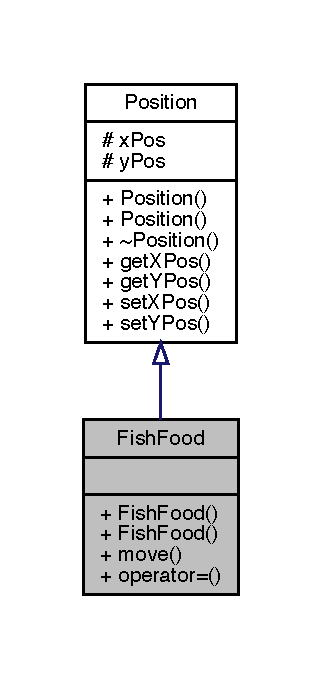
\includegraphics[width=154pt]{class_fish_food__coll__graph}
\end{center}
\end{figure}
\subsection*{Public Member Functions}
\begin{DoxyCompactItemize}
\item 
\mbox{\hyperlink{class_fish_food_a9aa0dcd43776eb7b0a98941cec3fbc1c}{Fish\+Food}} ()
\item 
\mbox{\hyperlink{class_fish_food_a3e2ae5b4b6c889595605f66bb9974b98}{Fish\+Food}} (double, double)
\item 
void \mbox{\hyperlink{class_fish_food_ab4dac48078ac8d5d1442c4fc4f4b8971}{move}} (double t)
\item 
\mbox{\hyperlink{class_fish_food}{Fish\+Food}} \mbox{\hyperlink{class_fish_food_aba5ba515f8d473b21ac658ed810e9cd3}{operator=}} (const \mbox{\hyperlink{class_fish_food}{Fish\+Food}} \&F)
\end{DoxyCompactItemize}
\subsection*{Additional Inherited Members}


\subsection{Constructor \& Destructor Documentation}
\mbox{\Hypertarget{class_fish_food_a9aa0dcd43776eb7b0a98941cec3fbc1c}\label{class_fish_food_a9aa0dcd43776eb7b0a98941cec3fbc1c}} 
\index{Fish\+Food@{Fish\+Food}!Fish\+Food@{Fish\+Food}}
\index{Fish\+Food@{Fish\+Food}!Fish\+Food@{Fish\+Food}}
\subsubsection{\texorpdfstring{Fish\+Food()}{FishFood()}\hspace{0.1cm}{\footnotesize\ttfamily [1/2]}}
{\footnotesize\ttfamily Fish\+Food\+::\+Fish\+Food (\begin{DoxyParamCaption}{ }\end{DoxyParamCaption})}

\mbox{\Hypertarget{class_fish_food_a3e2ae5b4b6c889595605f66bb9974b98}\label{class_fish_food_a3e2ae5b4b6c889595605f66bb9974b98}} 
\index{Fish\+Food@{Fish\+Food}!Fish\+Food@{Fish\+Food}}
\index{Fish\+Food@{Fish\+Food}!Fish\+Food@{Fish\+Food}}
\subsubsection{\texorpdfstring{Fish\+Food()}{FishFood()}\hspace{0.1cm}{\footnotesize\ttfamily [2/2]}}
{\footnotesize\ttfamily Fish\+Food\+::\+Fish\+Food (\begin{DoxyParamCaption}\item[{double}]{\+\_\+xpos,  }\item[{double}]{\+\_\+ypos }\end{DoxyParamCaption})}



\subsection{Member Function Documentation}
\mbox{\Hypertarget{class_fish_food_ab4dac48078ac8d5d1442c4fc4f4b8971}\label{class_fish_food_ab4dac48078ac8d5d1442c4fc4f4b8971}} 
\index{Fish\+Food@{Fish\+Food}!move@{move}}
\index{move@{move}!Fish\+Food@{Fish\+Food}}
\subsubsection{\texorpdfstring{move()}{move()}}
{\footnotesize\ttfamily void Fish\+Food\+::move (\begin{DoxyParamCaption}\item[{double}]{t }\end{DoxyParamCaption})}

\mbox{\Hypertarget{class_fish_food_aba5ba515f8d473b21ac658ed810e9cd3}\label{class_fish_food_aba5ba515f8d473b21ac658ed810e9cd3}} 
\index{Fish\+Food@{Fish\+Food}!operator=@{operator=}}
\index{operator=@{operator=}!Fish\+Food@{Fish\+Food}}
\subsubsection{\texorpdfstring{operator=()}{operator=()}}
{\footnotesize\ttfamily \mbox{\hyperlink{class_fish_food}{Fish\+Food}} Fish\+Food\+::operator= (\begin{DoxyParamCaption}\item[{const \mbox{\hyperlink{class_fish_food}{Fish\+Food}} \&}]{F }\end{DoxyParamCaption})}

Here is the call graph for this function\+:
\nopagebreak
\begin{figure}[H]
\begin{center}
\leavevmode
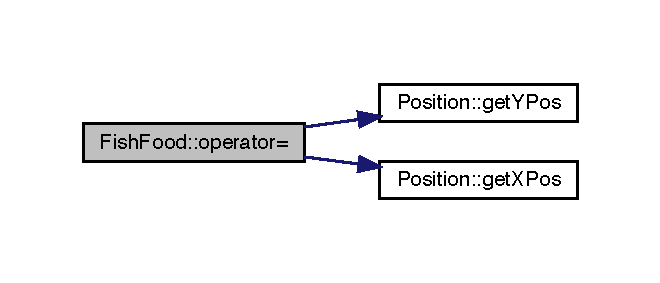
\includegraphics[width=317pt]{class_fish_food_aba5ba515f8d473b21ac658ed810e9cd3_cgraph}
\end{center}
\end{figure}


The documentation for this class was generated from the following files\+:\begin{DoxyCompactItemize}
\item 
\mbox{\hyperlink{_fish_food_8hpp}{Fish\+Food.\+hpp}}\item 
\mbox{\hyperlink{_fish_food_8cpp}{Fish\+Food.\+cpp}}\end{DoxyCompactItemize}

\hypertarget{class_guppy}{}\section{Guppy Class Reference}
\label{class_guppy}\index{Guppy@{Guppy}}


{\ttfamily \#include $<$Guppy.\+hpp$>$}



Inheritance diagram for Guppy\+:
\nopagebreak
\begin{figure}[H]
\begin{center}
\leavevmode
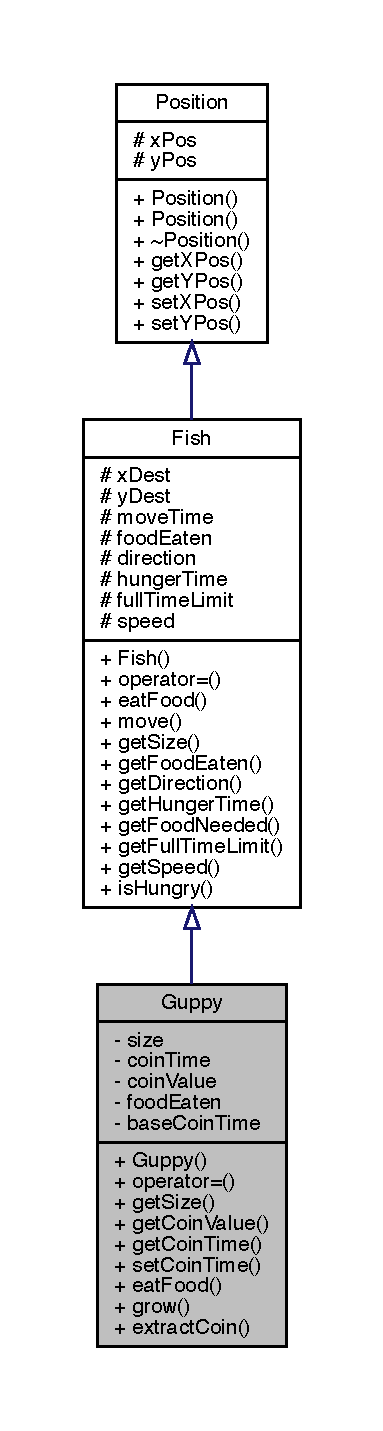
\includegraphics[height=550pt]{class_guppy__inherit__graph}
\end{center}
\end{figure}


Collaboration diagram for Guppy\+:
\nopagebreak
\begin{figure}[H]
\begin{center}
\leavevmode
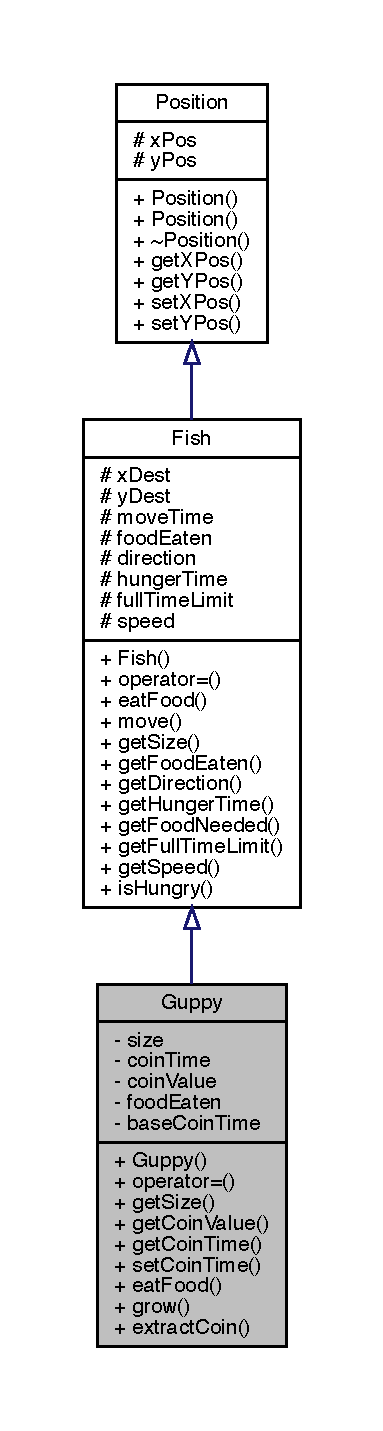
\includegraphics[height=550pt]{class_guppy__coll__graph}
\end{center}
\end{figure}
\subsection*{Public Member Functions}
\begin{DoxyCompactItemize}
\item 
\mbox{\hyperlink{class_guppy_aa78f8b5323b1015c968a8edab52773f5}{Guppy}} ()
\item 
\mbox{\hyperlink{class_guppy}{Guppy}} \mbox{\hyperlink{class_guppy_aa30f6db726124f670123daadb53a581f}{operator=}} (const \mbox{\hyperlink{class_guppy}{Guppy}} \&G)
\item 
int \mbox{\hyperlink{class_guppy_a38fa7d69e65a6778e1cdf6a0b542f295}{get\+Size}} () const
\item 
int \mbox{\hyperlink{class_guppy_ae190cb7bd1cbc2b36c36d99cd75848e0}{get\+Coin\+Value}} () const
\item 
double \mbox{\hyperlink{class_guppy_ae292cfe7a3d33ed860da190b930441b3}{get\+Coin\+Time}} () const
\item 
void \mbox{\hyperlink{class_guppy_a95cab69dac975dcdf44f0fdc698764e1}{set\+Coin\+Time}} (double t)
\item 
void \mbox{\hyperlink{class_guppy_a50115297f5c2f4df46e3613e09db115e}{eat\+Food}} ()
\item 
void \mbox{\hyperlink{class_guppy_a342d7b7c5a5c456b2acfa03a8e24494e}{grow}} ()
\item 
\mbox{\hyperlink{class_coin}{Coin}} \mbox{\hyperlink{class_guppy_ab3fef72b059ac88a3e901af4db113e1d}{extract\+Coin}} ()
\end{DoxyCompactItemize}
\subsection*{Private Attributes}
\begin{DoxyCompactItemize}
\item 
int \mbox{\hyperlink{class_guppy_af72ab3a1333652d6568daab2364f8667}{size}}
\item 
double \mbox{\hyperlink{class_guppy_a7499e4ee2b98b89ed5d90401c77e85e7}{coin\+Time}}
\item 
int \mbox{\hyperlink{class_guppy_af83c4763130d7c27b81b65c8395cf336}{coin\+Value}}
\item 
int \mbox{\hyperlink{class_guppy_a5eb6f3d64c0498fd4fcea47b645aa93f}{food\+Eaten}}
\item 
const double \mbox{\hyperlink{class_guppy_a89464da317c0ba87d07cb47d03d2fb18}{base\+Coin\+Time}} = 15.\+0
\end{DoxyCompactItemize}
\subsection*{Additional Inherited Members}


\subsection{Constructor \& Destructor Documentation}
\mbox{\Hypertarget{class_guppy_aa78f8b5323b1015c968a8edab52773f5}\label{class_guppy_aa78f8b5323b1015c968a8edab52773f5}} 
\index{Guppy@{Guppy}!Guppy@{Guppy}}
\index{Guppy@{Guppy}!Guppy@{Guppy}}
\subsubsection{\texorpdfstring{Guppy()}{Guppy()}}
{\footnotesize\ttfamily Guppy\+::\+Guppy (\begin{DoxyParamCaption}{ }\end{DoxyParamCaption})}



\subsection{Member Function Documentation}
\mbox{\Hypertarget{class_guppy_a50115297f5c2f4df46e3613e09db115e}\label{class_guppy_a50115297f5c2f4df46e3613e09db115e}} 
\index{Guppy@{Guppy}!eat\+Food@{eat\+Food}}
\index{eat\+Food@{eat\+Food}!Guppy@{Guppy}}
\subsubsection{\texorpdfstring{eat\+Food()}{eatFood()}}
{\footnotesize\ttfamily void Guppy\+::eat\+Food (\begin{DoxyParamCaption}{ }\end{DoxyParamCaption})\hspace{0.3cm}{\ttfamily [virtual]}}



Implements \mbox{\hyperlink{class_fish_aad629fb35c786b2a44c1204d011f9ae4}{Fish}}.

Here is the call graph for this function\+:
\nopagebreak
\begin{figure}[H]
\begin{center}
\leavevmode
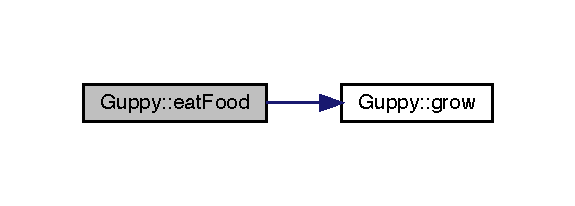
\includegraphics[width=276pt]{class_guppy_a50115297f5c2f4df46e3613e09db115e_cgraph}
\end{center}
\end{figure}
\mbox{\Hypertarget{class_guppy_ab3fef72b059ac88a3e901af4db113e1d}\label{class_guppy_ab3fef72b059ac88a3e901af4db113e1d}} 
\index{Guppy@{Guppy}!extract\+Coin@{extract\+Coin}}
\index{extract\+Coin@{extract\+Coin}!Guppy@{Guppy}}
\subsubsection{\texorpdfstring{extract\+Coin()}{extractCoin()}}
{\footnotesize\ttfamily \mbox{\hyperlink{class_coin}{Coin}} Guppy\+::extract\+Coin (\begin{DoxyParamCaption}{ }\end{DoxyParamCaption})}

Here is the call graph for this function\+:
\nopagebreak
\begin{figure}[H]
\begin{center}
\leavevmode
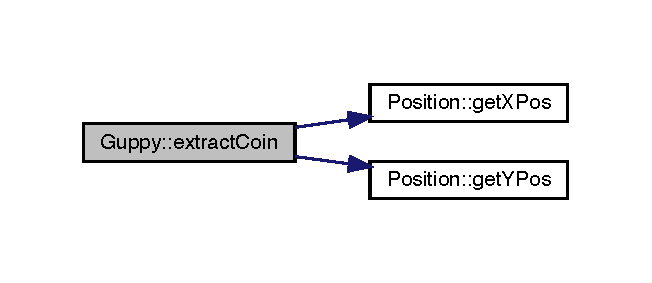
\includegraphics[width=313pt]{class_guppy_ab3fef72b059ac88a3e901af4db113e1d_cgraph}
\end{center}
\end{figure}
\mbox{\Hypertarget{class_guppy_ae292cfe7a3d33ed860da190b930441b3}\label{class_guppy_ae292cfe7a3d33ed860da190b930441b3}} 
\index{Guppy@{Guppy}!get\+Coin\+Time@{get\+Coin\+Time}}
\index{get\+Coin\+Time@{get\+Coin\+Time}!Guppy@{Guppy}}
\subsubsection{\texorpdfstring{get\+Coin\+Time()}{getCoinTime()}}
{\footnotesize\ttfamily double Guppy\+::get\+Coin\+Time (\begin{DoxyParamCaption}{ }\end{DoxyParamCaption}) const}

\mbox{\Hypertarget{class_guppy_ae190cb7bd1cbc2b36c36d99cd75848e0}\label{class_guppy_ae190cb7bd1cbc2b36c36d99cd75848e0}} 
\index{Guppy@{Guppy}!get\+Coin\+Value@{get\+Coin\+Value}}
\index{get\+Coin\+Value@{get\+Coin\+Value}!Guppy@{Guppy}}
\subsubsection{\texorpdfstring{get\+Coin\+Value()}{getCoinValue()}}
{\footnotesize\ttfamily int Guppy\+::get\+Coin\+Value (\begin{DoxyParamCaption}{ }\end{DoxyParamCaption}) const}

\mbox{\Hypertarget{class_guppy_a38fa7d69e65a6778e1cdf6a0b542f295}\label{class_guppy_a38fa7d69e65a6778e1cdf6a0b542f295}} 
\index{Guppy@{Guppy}!get\+Size@{get\+Size}}
\index{get\+Size@{get\+Size}!Guppy@{Guppy}}
\subsubsection{\texorpdfstring{get\+Size()}{getSize()}}
{\footnotesize\ttfamily int Guppy\+::get\+Size (\begin{DoxyParamCaption}{ }\end{DoxyParamCaption}) const}

\mbox{\Hypertarget{class_guppy_a342d7b7c5a5c456b2acfa03a8e24494e}\label{class_guppy_a342d7b7c5a5c456b2acfa03a8e24494e}} 
\index{Guppy@{Guppy}!grow@{grow}}
\index{grow@{grow}!Guppy@{Guppy}}
\subsubsection{\texorpdfstring{grow()}{grow()}}
{\footnotesize\ttfamily void Guppy\+::grow (\begin{DoxyParamCaption}{ }\end{DoxyParamCaption})}

\mbox{\Hypertarget{class_guppy_aa30f6db726124f670123daadb53a581f}\label{class_guppy_aa30f6db726124f670123daadb53a581f}} 
\index{Guppy@{Guppy}!operator=@{operator=}}
\index{operator=@{operator=}!Guppy@{Guppy}}
\subsubsection{\texorpdfstring{operator=()}{operator=()}}
{\footnotesize\ttfamily \mbox{\hyperlink{class_guppy}{Guppy}} Guppy\+::operator= (\begin{DoxyParamCaption}\item[{const \mbox{\hyperlink{class_guppy}{Guppy}} \&}]{G }\end{DoxyParamCaption})}

Here is the call graph for this function\+:
\nopagebreak
\begin{figure}[H]
\begin{center}
\leavevmode
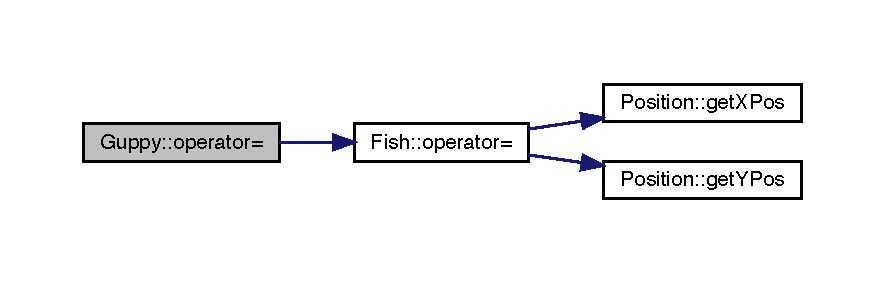
\includegraphics[width=350pt]{class_guppy_aa30f6db726124f670123daadb53a581f_cgraph}
\end{center}
\end{figure}
\mbox{\Hypertarget{class_guppy_a95cab69dac975dcdf44f0fdc698764e1}\label{class_guppy_a95cab69dac975dcdf44f0fdc698764e1}} 
\index{Guppy@{Guppy}!set\+Coin\+Time@{set\+Coin\+Time}}
\index{set\+Coin\+Time@{set\+Coin\+Time}!Guppy@{Guppy}}
\subsubsection{\texorpdfstring{set\+Coin\+Time()}{setCoinTime()}}
{\footnotesize\ttfamily void Guppy\+::set\+Coin\+Time (\begin{DoxyParamCaption}\item[{double}]{t }\end{DoxyParamCaption})}



\subsection{Member Data Documentation}
\mbox{\Hypertarget{class_guppy_a89464da317c0ba87d07cb47d03d2fb18}\label{class_guppy_a89464da317c0ba87d07cb47d03d2fb18}} 
\index{Guppy@{Guppy}!base\+Coin\+Time@{base\+Coin\+Time}}
\index{base\+Coin\+Time@{base\+Coin\+Time}!Guppy@{Guppy}}
\subsubsection{\texorpdfstring{base\+Coin\+Time}{baseCoinTime}}
{\footnotesize\ttfamily const double Guppy\+::base\+Coin\+Time = 15.\+0\hspace{0.3cm}{\ttfamily [private]}}

\mbox{\Hypertarget{class_guppy_a7499e4ee2b98b89ed5d90401c77e85e7}\label{class_guppy_a7499e4ee2b98b89ed5d90401c77e85e7}} 
\index{Guppy@{Guppy}!coin\+Time@{coin\+Time}}
\index{coin\+Time@{coin\+Time}!Guppy@{Guppy}}
\subsubsection{\texorpdfstring{coin\+Time}{coinTime}}
{\footnotesize\ttfamily double Guppy\+::coin\+Time\hspace{0.3cm}{\ttfamily [private]}}

\mbox{\Hypertarget{class_guppy_af83c4763130d7c27b81b65c8395cf336}\label{class_guppy_af83c4763130d7c27b81b65c8395cf336}} 
\index{Guppy@{Guppy}!coin\+Value@{coin\+Value}}
\index{coin\+Value@{coin\+Value}!Guppy@{Guppy}}
\subsubsection{\texorpdfstring{coin\+Value}{coinValue}}
{\footnotesize\ttfamily int Guppy\+::coin\+Value\hspace{0.3cm}{\ttfamily [private]}}

\mbox{\Hypertarget{class_guppy_a5eb6f3d64c0498fd4fcea47b645aa93f}\label{class_guppy_a5eb6f3d64c0498fd4fcea47b645aa93f}} 
\index{Guppy@{Guppy}!food\+Eaten@{food\+Eaten}}
\index{food\+Eaten@{food\+Eaten}!Guppy@{Guppy}}
\subsubsection{\texorpdfstring{food\+Eaten}{foodEaten}}
{\footnotesize\ttfamily int Guppy\+::food\+Eaten\hspace{0.3cm}{\ttfamily [private]}}

\mbox{\Hypertarget{class_guppy_af72ab3a1333652d6568daab2364f8667}\label{class_guppy_af72ab3a1333652d6568daab2364f8667}} 
\index{Guppy@{Guppy}!size@{size}}
\index{size@{size}!Guppy@{Guppy}}
\subsubsection{\texorpdfstring{size}{size}}
{\footnotesize\ttfamily int Guppy\+::size\hspace{0.3cm}{\ttfamily [private]}}



The documentation for this class was generated from the following files\+:\begin{DoxyCompactItemize}
\item 
\mbox{\hyperlink{_guppy_8hpp}{Guppy.\+hpp}}\item 
\mbox{\hyperlink{_guppy_8cpp}{Guppy.\+cpp}}\end{DoxyCompactItemize}

\hypertarget{class_linked_list}{}\section{Linked\+List$<$ T $>$ Class Template Reference}
\label{class_linked_list}\index{Linked\+List$<$ T $>$@{Linked\+List$<$ T $>$}}


{\ttfamily \#include $<$Linked\+List.\+hpp$>$}



Inheritance diagram for Linked\+List$<$ T $>$\+:
\nopagebreak
\begin{figure}[H]
\begin{center}
\leavevmode
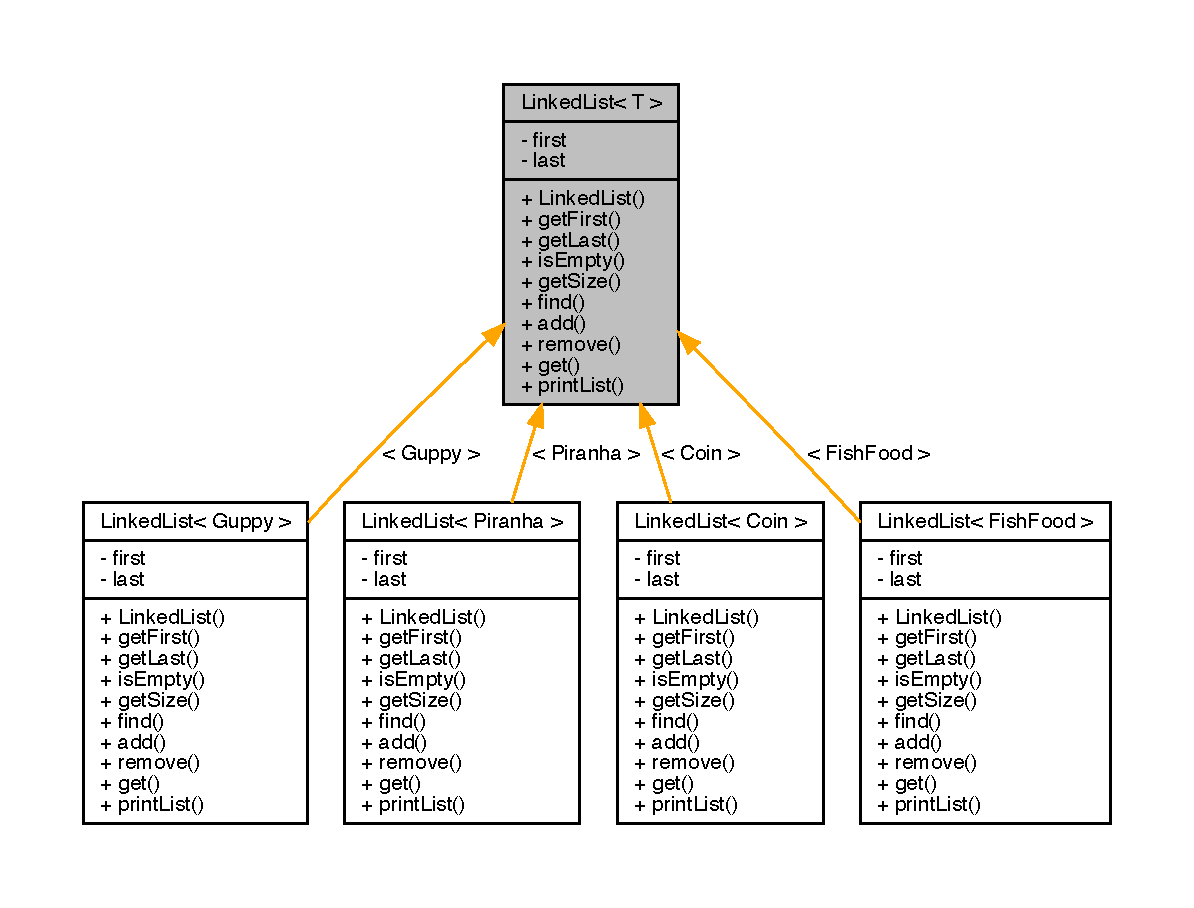
\includegraphics[width=350pt]{class_linked_list__inherit__graph}
\end{center}
\end{figure}


Collaboration diagram for Linked\+List$<$ T $>$\+:
\nopagebreak
\begin{figure}[H]
\begin{center}
\leavevmode
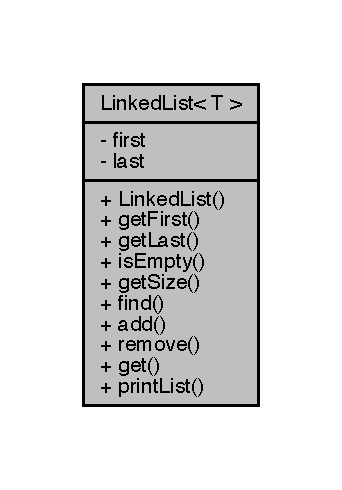
\includegraphics[width=164pt]{class_linked_list__coll__graph}
\end{center}
\end{figure}
\subsection*{Public Member Functions}
\begin{DoxyCompactItemize}
\item 
\mbox{\hyperlink{class_linked_list_a3c20fcfec867e867f541061a09fc640c}{Linked\+List}} ()
\item 
\mbox{\hyperlink{structnode}{node}}$<$ T $>$ \mbox{\hyperlink{class_linked_list_a793ceff04b597446486983d4d651e943}{get\+First}} ()
\item 
\mbox{\hyperlink{structnode}{node}}$<$ T $>$ \mbox{\hyperlink{class_linked_list_ad5443b28b382db29e5a5a552b9a3dddc}{get\+Last}} ()
\item 
bool \mbox{\hyperlink{class_linked_list_a7ecbb28e82117a680839ed0dc28ebdce}{is\+Empty}} ()
\item 
int \mbox{\hyperlink{class_linked_list_a2b77410d908509ee9f11497ead71a282}{get\+Size}} () const
\item 
int \mbox{\hyperlink{class_linked_list_a924e217dd525b84492e9f0dc61db96bc}{find}} (T element)
\item 
void \mbox{\hyperlink{class_linked_list_ab7364799e5965dd59d4f5952cb953287}{add}} (T element)
\item 
void \mbox{\hyperlink{class_linked_list_ad2958c4e9413017f354613a5ffe0fc9e}{remove}} (T \&element)
\item 
T \& \mbox{\hyperlink{class_linked_list_aa34d85df4f82f094ba9d6f4708519ebd}{get}} (int index)
\item 
void \mbox{\hyperlink{class_linked_list_af360d4c51f63b7756ac555efbfd5d4b6}{print\+List}} ()
\end{DoxyCompactItemize}
\subsection*{Private Attributes}
\begin{DoxyCompactItemize}
\item 
\mbox{\hyperlink{structnode}{node}}$<$ T $>$ $\ast$ \mbox{\hyperlink{class_linked_list_acaeb0499689a66aa0f0c6f71864da9a2}{first}}
\item 
\mbox{\hyperlink{structnode}{node}}$<$ T $>$ $\ast$ \mbox{\hyperlink{class_linked_list_ab584a6000168e8e43549dffda60240b2}{last}}
\end{DoxyCompactItemize}


\subsection{Constructor \& Destructor Documentation}
\mbox{\Hypertarget{class_linked_list_a3c20fcfec867e867f541061a09fc640c}\label{class_linked_list_a3c20fcfec867e867f541061a09fc640c}} 
\index{Linked\+List@{Linked\+List}!Linked\+List@{Linked\+List}}
\index{Linked\+List@{Linked\+List}!Linked\+List@{Linked\+List}}
\subsubsection{\texorpdfstring{Linked\+List()}{LinkedList()}}
{\footnotesize\ttfamily template$<$class T$>$ \\
\mbox{\hyperlink{class_linked_list}{Linked\+List}}$<$ T $>$\+::\mbox{\hyperlink{class_linked_list}{Linked\+List}} (\begin{DoxyParamCaption}{ }\end{DoxyParamCaption})\hspace{0.3cm}{\ttfamily [inline]}}



\subsection{Member Function Documentation}
\mbox{\Hypertarget{class_linked_list_ab7364799e5965dd59d4f5952cb953287}\label{class_linked_list_ab7364799e5965dd59d4f5952cb953287}} 
\index{Linked\+List@{Linked\+List}!add@{add}}
\index{add@{add}!Linked\+List@{Linked\+List}}
\subsubsection{\texorpdfstring{add()}{add()}}
{\footnotesize\ttfamily template$<$class T$>$ \\
void \mbox{\hyperlink{class_linked_list}{Linked\+List}}$<$ T $>$\+::add (\begin{DoxyParamCaption}\item[{T}]{element }\end{DoxyParamCaption})\hspace{0.3cm}{\ttfamily [inline]}}

\mbox{\Hypertarget{class_linked_list_a924e217dd525b84492e9f0dc61db96bc}\label{class_linked_list_a924e217dd525b84492e9f0dc61db96bc}} 
\index{Linked\+List@{Linked\+List}!find@{find}}
\index{find@{find}!Linked\+List@{Linked\+List}}
\subsubsection{\texorpdfstring{find()}{find()}}
{\footnotesize\ttfamily template$<$class T$>$ \\
int \mbox{\hyperlink{class_linked_list}{Linked\+List}}$<$ T $>$\+::find (\begin{DoxyParamCaption}\item[{T}]{element }\end{DoxyParamCaption})\hspace{0.3cm}{\ttfamily [inline]}}

\mbox{\Hypertarget{class_linked_list_aa34d85df4f82f094ba9d6f4708519ebd}\label{class_linked_list_aa34d85df4f82f094ba9d6f4708519ebd}} 
\index{Linked\+List@{Linked\+List}!get@{get}}
\index{get@{get}!Linked\+List@{Linked\+List}}
\subsubsection{\texorpdfstring{get()}{get()}}
{\footnotesize\ttfamily template$<$class T$>$ \\
T\& \mbox{\hyperlink{class_linked_list}{Linked\+List}}$<$ T $>$\+::get (\begin{DoxyParamCaption}\item[{int}]{index }\end{DoxyParamCaption})\hspace{0.3cm}{\ttfamily [inline]}}

\mbox{\Hypertarget{class_linked_list_a793ceff04b597446486983d4d651e943}\label{class_linked_list_a793ceff04b597446486983d4d651e943}} 
\index{Linked\+List@{Linked\+List}!get\+First@{get\+First}}
\index{get\+First@{get\+First}!Linked\+List@{Linked\+List}}
\subsubsection{\texorpdfstring{get\+First()}{getFirst()}}
{\footnotesize\ttfamily template$<$class T$>$ \\
\mbox{\hyperlink{structnode}{node}}$<$T$>$ \mbox{\hyperlink{class_linked_list}{Linked\+List}}$<$ T $>$\+::get\+First (\begin{DoxyParamCaption}{ }\end{DoxyParamCaption})\hspace{0.3cm}{\ttfamily [inline]}}

\mbox{\Hypertarget{class_linked_list_ad5443b28b382db29e5a5a552b9a3dddc}\label{class_linked_list_ad5443b28b382db29e5a5a552b9a3dddc}} 
\index{Linked\+List@{Linked\+List}!get\+Last@{get\+Last}}
\index{get\+Last@{get\+Last}!Linked\+List@{Linked\+List}}
\subsubsection{\texorpdfstring{get\+Last()}{getLast()}}
{\footnotesize\ttfamily template$<$class T$>$ \\
\mbox{\hyperlink{structnode}{node}}$<$T$>$ \mbox{\hyperlink{class_linked_list}{Linked\+List}}$<$ T $>$\+::get\+Last (\begin{DoxyParamCaption}{ }\end{DoxyParamCaption})\hspace{0.3cm}{\ttfamily [inline]}}

\mbox{\Hypertarget{class_linked_list_a2b77410d908509ee9f11497ead71a282}\label{class_linked_list_a2b77410d908509ee9f11497ead71a282}} 
\index{Linked\+List@{Linked\+List}!get\+Size@{get\+Size}}
\index{get\+Size@{get\+Size}!Linked\+List@{Linked\+List}}
\subsubsection{\texorpdfstring{get\+Size()}{getSize()}}
{\footnotesize\ttfamily template$<$class T$>$ \\
int \mbox{\hyperlink{class_linked_list}{Linked\+List}}$<$ T $>$\+::get\+Size (\begin{DoxyParamCaption}{ }\end{DoxyParamCaption}) const\hspace{0.3cm}{\ttfamily [inline]}}

\mbox{\Hypertarget{class_linked_list_a7ecbb28e82117a680839ed0dc28ebdce}\label{class_linked_list_a7ecbb28e82117a680839ed0dc28ebdce}} 
\index{Linked\+List@{Linked\+List}!is\+Empty@{is\+Empty}}
\index{is\+Empty@{is\+Empty}!Linked\+List@{Linked\+List}}
\subsubsection{\texorpdfstring{is\+Empty()}{isEmpty()}}
{\footnotesize\ttfamily template$<$class T$>$ \\
bool \mbox{\hyperlink{class_linked_list}{Linked\+List}}$<$ T $>$\+::is\+Empty (\begin{DoxyParamCaption}{ }\end{DoxyParamCaption})\hspace{0.3cm}{\ttfamily [inline]}}

\mbox{\Hypertarget{class_linked_list_af360d4c51f63b7756ac555efbfd5d4b6}\label{class_linked_list_af360d4c51f63b7756ac555efbfd5d4b6}} 
\index{Linked\+List@{Linked\+List}!print\+List@{print\+List}}
\index{print\+List@{print\+List}!Linked\+List@{Linked\+List}}
\subsubsection{\texorpdfstring{print\+List()}{printList()}}
{\footnotesize\ttfamily template$<$class T$>$ \\
void \mbox{\hyperlink{class_linked_list}{Linked\+List}}$<$ T $>$\+::print\+List (\begin{DoxyParamCaption}{ }\end{DoxyParamCaption})\hspace{0.3cm}{\ttfamily [inline]}}

\mbox{\Hypertarget{class_linked_list_ad2958c4e9413017f354613a5ffe0fc9e}\label{class_linked_list_ad2958c4e9413017f354613a5ffe0fc9e}} 
\index{Linked\+List@{Linked\+List}!remove@{remove}}
\index{remove@{remove}!Linked\+List@{Linked\+List}}
\subsubsection{\texorpdfstring{remove()}{remove()}}
{\footnotesize\ttfamily template$<$class T$>$ \\
void \mbox{\hyperlink{class_linked_list}{Linked\+List}}$<$ T $>$\+::remove (\begin{DoxyParamCaption}\item[{T \&}]{element }\end{DoxyParamCaption})\hspace{0.3cm}{\ttfamily [inline]}}



\subsection{Member Data Documentation}
\mbox{\Hypertarget{class_linked_list_acaeb0499689a66aa0f0c6f71864da9a2}\label{class_linked_list_acaeb0499689a66aa0f0c6f71864da9a2}} 
\index{Linked\+List@{Linked\+List}!first@{first}}
\index{first@{first}!Linked\+List@{Linked\+List}}
\subsubsection{\texorpdfstring{first}{first}}
{\footnotesize\ttfamily template$<$class T$>$ \\
\mbox{\hyperlink{structnode}{node}}$<$T$>$$\ast$ \mbox{\hyperlink{class_linked_list}{Linked\+List}}$<$ T $>$\+::first\hspace{0.3cm}{\ttfamily [private]}}

\mbox{\Hypertarget{class_linked_list_ab584a6000168e8e43549dffda60240b2}\label{class_linked_list_ab584a6000168e8e43549dffda60240b2}} 
\index{Linked\+List@{Linked\+List}!last@{last}}
\index{last@{last}!Linked\+List@{Linked\+List}}
\subsubsection{\texorpdfstring{last}{last}}
{\footnotesize\ttfamily template$<$class T$>$ \\
\mbox{\hyperlink{structnode}{node}}$<$T$>$$\ast$ \mbox{\hyperlink{class_linked_list}{Linked\+List}}$<$ T $>$\+::last\hspace{0.3cm}{\ttfamily [private]}}



The documentation for this class was generated from the following file\+:\begin{DoxyCompactItemize}
\item 
\mbox{\hyperlink{_linked_list_8hpp}{Linked\+List.\+hpp}}\end{DoxyCompactItemize}

\hypertarget{structnode}{}\section{node$<$ T $>$ Struct Template Reference}
\label{structnode}\index{node$<$ T $>$@{node$<$ T $>$}}


{\ttfamily \#include $<$Linked\+List.\+hpp$>$}



Inheritance diagram for node$<$ T $>$\+:
\nopagebreak
\begin{figure}[H]
\begin{center}
\leavevmode
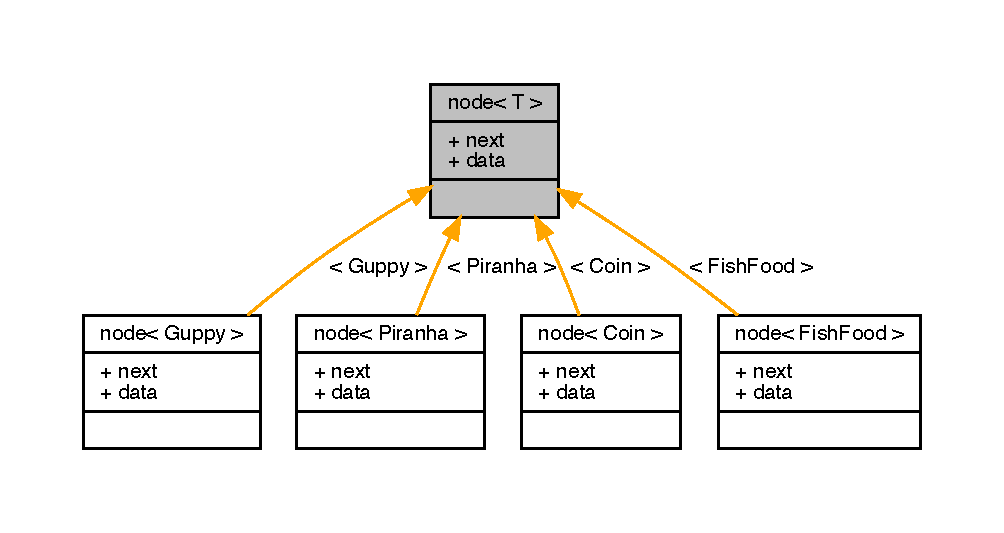
\includegraphics[width=350pt]{structnode__inherit__graph}
\end{center}
\end{figure}


Collaboration diagram for node$<$ T $>$\+:
\nopagebreak
\begin{figure}[H]
\begin{center}
\leavevmode
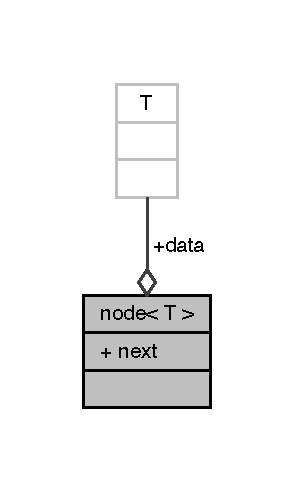
\includegraphics[width=141pt]{structnode__coll__graph}
\end{center}
\end{figure}
\subsection*{Public Attributes}
\begin{DoxyCompactItemize}
\item 
\mbox{\hyperlink{structnode}{node}}$<$ T $>$ $\ast$ \mbox{\hyperlink{structnode_ac96190e012822e6c053d2a5e9eedd68d}{next}}
\item 
T \mbox{\hyperlink{structnode_a0a3e961e5caf1562f0c27caef3940e7a}{data}}
\end{DoxyCompactItemize}


\subsection{Member Data Documentation}
\mbox{\Hypertarget{structnode_a0a3e961e5caf1562f0c27caef3940e7a}\label{structnode_a0a3e961e5caf1562f0c27caef3940e7a}} 
\index{node@{node}!data@{data}}
\index{data@{data}!node@{node}}
\subsubsection{\texorpdfstring{data}{data}}
{\footnotesize\ttfamily template$<$class T$>$ \\
T \mbox{\hyperlink{structnode}{node}}$<$ T $>$\+::data}

\mbox{\Hypertarget{structnode_ac96190e012822e6c053d2a5e9eedd68d}\label{structnode_ac96190e012822e6c053d2a5e9eedd68d}} 
\index{node@{node}!next@{next}}
\index{next@{next}!node@{node}}
\subsubsection{\texorpdfstring{next}{next}}
{\footnotesize\ttfamily template$<$class T$>$ \\
\mbox{\hyperlink{structnode}{node}}$<$T$>$$\ast$ \mbox{\hyperlink{structnode}{node}}$<$ T $>$\+::next}



The documentation for this struct was generated from the following file\+:\begin{DoxyCompactItemize}
\item 
\mbox{\hyperlink{_linked_list_8hpp}{Linked\+List.\+hpp}}\end{DoxyCompactItemize}

\hypertarget{class_piranha}{}\section{Piranha Class Reference}
\label{class_piranha}\index{Piranha@{Piranha}}


{\ttfamily \#include $<$Piranha.\+hpp$>$}



Inheritance diagram for Piranha\+:
\nopagebreak
\begin{figure}[H]
\begin{center}
\leavevmode
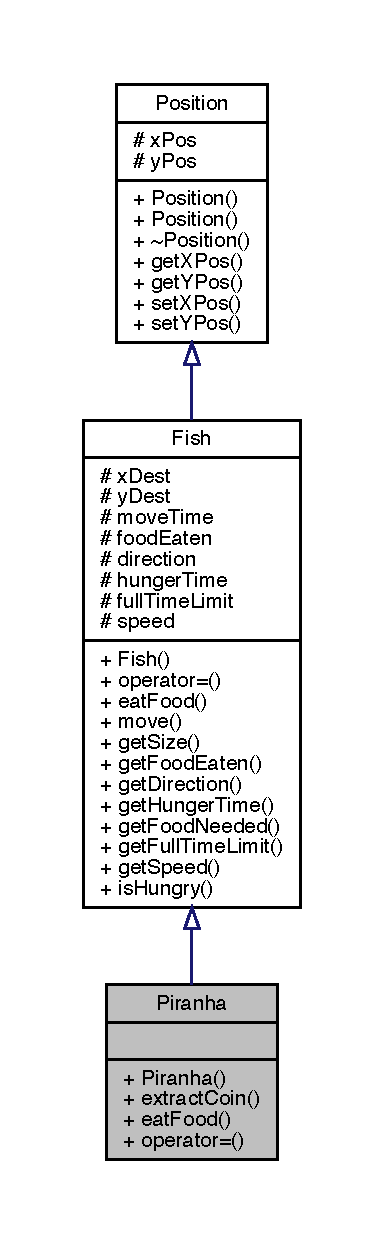
\includegraphics[height=550pt]{class_piranha__inherit__graph}
\end{center}
\end{figure}


Collaboration diagram for Piranha\+:
\nopagebreak
\begin{figure}[H]
\begin{center}
\leavevmode
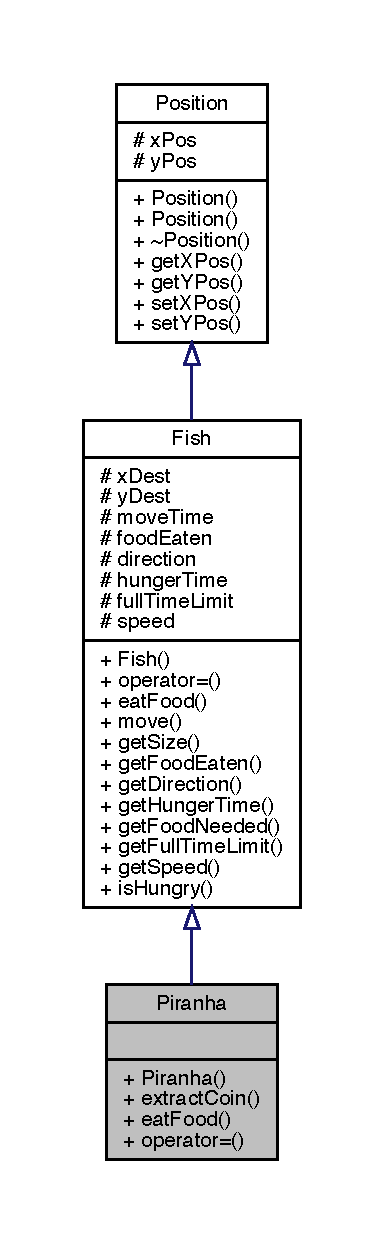
\includegraphics[height=550pt]{class_piranha__coll__graph}
\end{center}
\end{figure}
\subsection*{Public Member Functions}
\begin{DoxyCompactItemize}
\item 
\mbox{\hyperlink{class_piranha_a7e3a4c5c7f458c16717c8cb997fc0331}{Piranha}} ()
\item 
\mbox{\hyperlink{class_coin}{Coin}} \mbox{\hyperlink{class_piranha_aed1eb8799f7b92fbfb47fd760bf31cbf}{extract\+Coin}} (int)
\item 
void \mbox{\hyperlink{class_piranha_a50992b83e072f8719150d302469a462f}{eat\+Food}} ()
\item 
\mbox{\hyperlink{class_piranha}{Piranha}} \mbox{\hyperlink{class_piranha_a3f3a74ccd3e74052a78134c597fa6827}{operator=}} (const \mbox{\hyperlink{class_piranha}{Piranha}} \&P)
\end{DoxyCompactItemize}
\subsection*{Additional Inherited Members}


\subsection{Constructor \& Destructor Documentation}
\mbox{\Hypertarget{class_piranha_a7e3a4c5c7f458c16717c8cb997fc0331}\label{class_piranha_a7e3a4c5c7f458c16717c8cb997fc0331}} 
\index{Piranha@{Piranha}!Piranha@{Piranha}}
\index{Piranha@{Piranha}!Piranha@{Piranha}}
\subsubsection{\texorpdfstring{Piranha()}{Piranha()}}
{\footnotesize\ttfamily Piranha\+::\+Piranha (\begin{DoxyParamCaption}{ }\end{DoxyParamCaption})}



\subsection{Member Function Documentation}
\mbox{\Hypertarget{class_piranha_a50992b83e072f8719150d302469a462f}\label{class_piranha_a50992b83e072f8719150d302469a462f}} 
\index{Piranha@{Piranha}!eat\+Food@{eat\+Food}}
\index{eat\+Food@{eat\+Food}!Piranha@{Piranha}}
\subsubsection{\texorpdfstring{eat\+Food()}{eatFood()}}
{\footnotesize\ttfamily void Piranha\+::eat\+Food (\begin{DoxyParamCaption}{ }\end{DoxyParamCaption})\hspace{0.3cm}{\ttfamily [virtual]}}



Implements \mbox{\hyperlink{class_fish_aad629fb35c786b2a44c1204d011f9ae4}{Fish}}.

\mbox{\Hypertarget{class_piranha_aed1eb8799f7b92fbfb47fd760bf31cbf}\label{class_piranha_aed1eb8799f7b92fbfb47fd760bf31cbf}} 
\index{Piranha@{Piranha}!extract\+Coin@{extract\+Coin}}
\index{extract\+Coin@{extract\+Coin}!Piranha@{Piranha}}
\subsubsection{\texorpdfstring{extract\+Coin()}{extractCoin()}}
{\footnotesize\ttfamily \mbox{\hyperlink{class_coin}{Coin}} Piranha\+::extract\+Coin (\begin{DoxyParamCaption}\item[{int}]{val }\end{DoxyParamCaption})}

Here is the call graph for this function\+:
\nopagebreak
\begin{figure}[H]
\begin{center}
\leavevmode
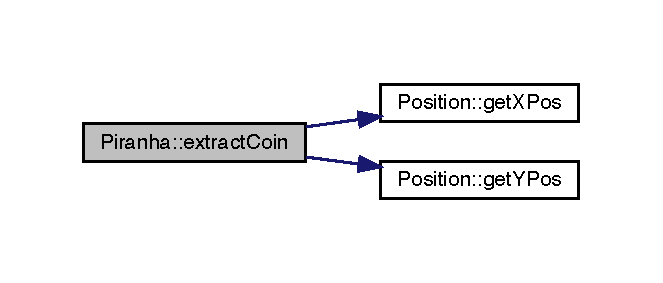
\includegraphics[width=318pt]{class_piranha_aed1eb8799f7b92fbfb47fd760bf31cbf_cgraph}
\end{center}
\end{figure}
\mbox{\Hypertarget{class_piranha_a3f3a74ccd3e74052a78134c597fa6827}\label{class_piranha_a3f3a74ccd3e74052a78134c597fa6827}} 
\index{Piranha@{Piranha}!operator=@{operator=}}
\index{operator=@{operator=}!Piranha@{Piranha}}
\subsubsection{\texorpdfstring{operator=()}{operator=()}}
{\footnotesize\ttfamily \mbox{\hyperlink{class_piranha}{Piranha}} Piranha\+::operator= (\begin{DoxyParamCaption}\item[{const \mbox{\hyperlink{class_piranha}{Piranha}} \&}]{P }\end{DoxyParamCaption})}

Here is the call graph for this function\+:
\nopagebreak
\begin{figure}[H]
\begin{center}
\leavevmode
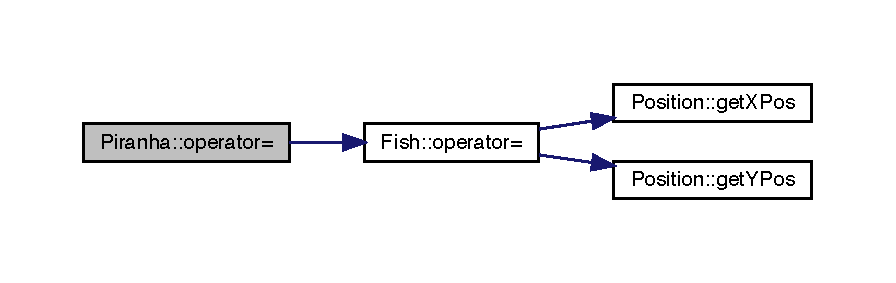
\includegraphics[width=350pt]{class_piranha_a3f3a74ccd3e74052a78134c597fa6827_cgraph}
\end{center}
\end{figure}


The documentation for this class was generated from the following files\+:\begin{DoxyCompactItemize}
\item 
\mbox{\hyperlink{_piranha_8hpp}{Piranha.\+hpp}}\item 
\mbox{\hyperlink{_piranha_8cpp}{Piranha.\+cpp}}\end{DoxyCompactItemize}

\hypertarget{class_position}{}\section{Position Class Reference}
\label{class_position}\index{Position@{Position}}


{\ttfamily \#include $<$Position.\+hpp$>$}



Inheritance diagram for Position\+:
\nopagebreak
\begin{figure}[H]
\begin{center}
\leavevmode
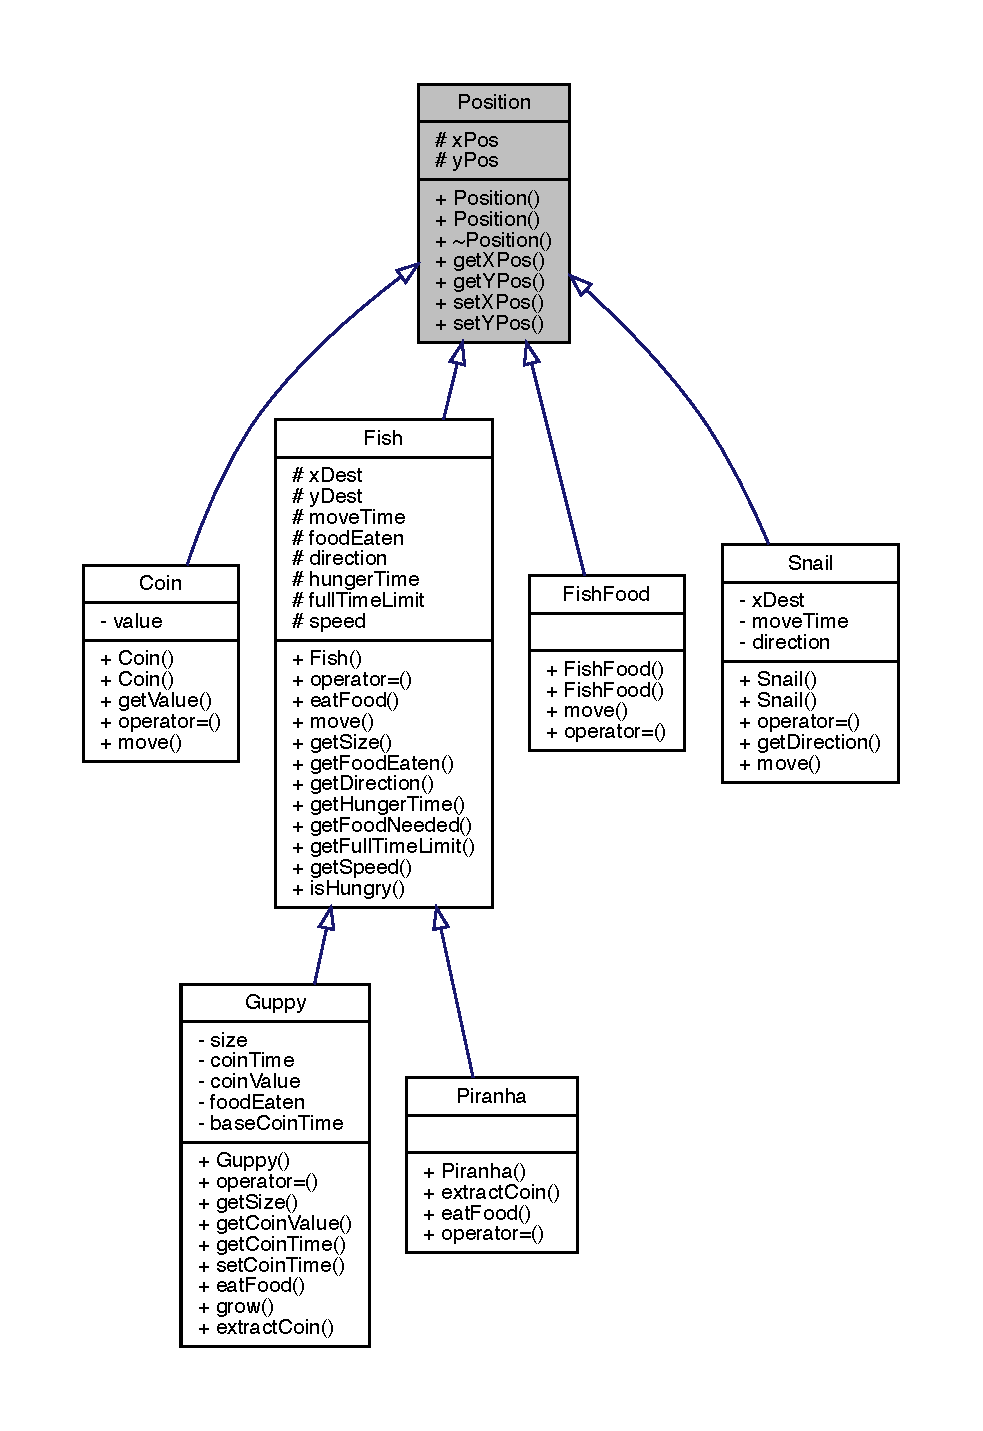
\includegraphics[width=350pt]{class_position__inherit__graph}
\end{center}
\end{figure}


Collaboration diagram for Position\+:
\nopagebreak
\begin{figure}[H]
\begin{center}
\leavevmode
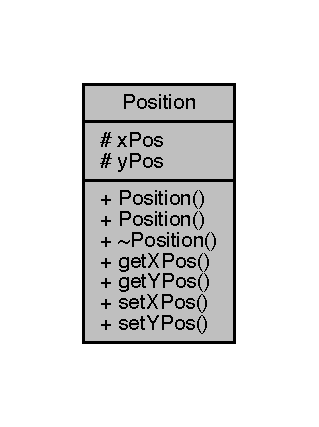
\includegraphics[width=153pt]{class_position__coll__graph}
\end{center}
\end{figure}
\subsection*{Public Member Functions}
\begin{DoxyCompactItemize}
\item 
\mbox{\hyperlink{class_position_a369a577425f8ba02e8750d04b6a088db}{Position}} ()
\item 
\mbox{\hyperlink{class_position_a75efef3ff44bc0bd38f7f10abb3a53fe}{Position}} (double \+\_\+x, double \+\_\+y)
\item 
\mbox{\hyperlink{class_position_abe83df4cab7af756636b4e39e4378f4a}{$\sim$\+Position}} ()
\item 
double \mbox{\hyperlink{class_position_a961116b828f39200092daddffca2a63c}{get\+X\+Pos}} () const
\item 
double \mbox{\hyperlink{class_position_a9bf258e61c4d01643599c175007254ac}{get\+Y\+Pos}} () const
\item 
void \mbox{\hyperlink{class_position_a9452ac5b29a317165ea9ee8386b82581}{set\+X\+Pos}} (double \+\_\+x)
\item 
void \mbox{\hyperlink{class_position_ae30f190ecd76be1de484773d9544a7f6}{set\+Y\+Pos}} (double \+\_\+y)
\end{DoxyCompactItemize}
\subsection*{Protected Attributes}
\begin{DoxyCompactItemize}
\item 
double \mbox{\hyperlink{class_position_a14ec3b05a733470d871518491601669f}{x\+Pos}}
\item 
double \mbox{\hyperlink{class_position_ad6bf63afed8bcc92e4fb74b7d5d7eabc}{y\+Pos}}
\end{DoxyCompactItemize}


\subsection{Constructor \& Destructor Documentation}
\mbox{\Hypertarget{class_position_a369a577425f8ba02e8750d04b6a088db}\label{class_position_a369a577425f8ba02e8750d04b6a088db}} 
\index{Position@{Position}!Position@{Position}}
\index{Position@{Position}!Position@{Position}}
\subsubsection{\texorpdfstring{Position()}{Position()}\hspace{0.1cm}{\footnotesize\ttfamily [1/2]}}
{\footnotesize\ttfamily Position\+::\+Position (\begin{DoxyParamCaption}{ }\end{DoxyParamCaption})}

\mbox{\Hypertarget{class_position_a75efef3ff44bc0bd38f7f10abb3a53fe}\label{class_position_a75efef3ff44bc0bd38f7f10abb3a53fe}} 
\index{Position@{Position}!Position@{Position}}
\index{Position@{Position}!Position@{Position}}
\subsubsection{\texorpdfstring{Position()}{Position()}\hspace{0.1cm}{\footnotesize\ttfamily [2/2]}}
{\footnotesize\ttfamily Position\+::\+Position (\begin{DoxyParamCaption}\item[{double}]{\+\_\+x,  }\item[{double}]{\+\_\+y }\end{DoxyParamCaption})}

\mbox{\Hypertarget{class_position_abe83df4cab7af756636b4e39e4378f4a}\label{class_position_abe83df4cab7af756636b4e39e4378f4a}} 
\index{Position@{Position}!````~Position@{$\sim$\+Position}}
\index{````~Position@{$\sim$\+Position}!Position@{Position}}
\subsubsection{\texorpdfstring{$\sim$\+Position()}{~Position()}}
{\footnotesize\ttfamily Position\+::$\sim$\+Position (\begin{DoxyParamCaption}{ }\end{DoxyParamCaption})}



\subsection{Member Function Documentation}
\mbox{\Hypertarget{class_position_a961116b828f39200092daddffca2a63c}\label{class_position_a961116b828f39200092daddffca2a63c}} 
\index{Position@{Position}!get\+X\+Pos@{get\+X\+Pos}}
\index{get\+X\+Pos@{get\+X\+Pos}!Position@{Position}}
\subsubsection{\texorpdfstring{get\+X\+Pos()}{getXPos()}}
{\footnotesize\ttfamily double Position\+::get\+X\+Pos (\begin{DoxyParamCaption}{ }\end{DoxyParamCaption}) const}

\mbox{\Hypertarget{class_position_a9bf258e61c4d01643599c175007254ac}\label{class_position_a9bf258e61c4d01643599c175007254ac}} 
\index{Position@{Position}!get\+Y\+Pos@{get\+Y\+Pos}}
\index{get\+Y\+Pos@{get\+Y\+Pos}!Position@{Position}}
\subsubsection{\texorpdfstring{get\+Y\+Pos()}{getYPos()}}
{\footnotesize\ttfamily double Position\+::get\+Y\+Pos (\begin{DoxyParamCaption}{ }\end{DoxyParamCaption}) const}

\mbox{\Hypertarget{class_position_a9452ac5b29a317165ea9ee8386b82581}\label{class_position_a9452ac5b29a317165ea9ee8386b82581}} 
\index{Position@{Position}!set\+X\+Pos@{set\+X\+Pos}}
\index{set\+X\+Pos@{set\+X\+Pos}!Position@{Position}}
\subsubsection{\texorpdfstring{set\+X\+Pos()}{setXPos()}}
{\footnotesize\ttfamily void Position\+::set\+X\+Pos (\begin{DoxyParamCaption}\item[{double}]{\+\_\+x }\end{DoxyParamCaption})}

\mbox{\Hypertarget{class_position_ae30f190ecd76be1de484773d9544a7f6}\label{class_position_ae30f190ecd76be1de484773d9544a7f6}} 
\index{Position@{Position}!set\+Y\+Pos@{set\+Y\+Pos}}
\index{set\+Y\+Pos@{set\+Y\+Pos}!Position@{Position}}
\subsubsection{\texorpdfstring{set\+Y\+Pos()}{setYPos()}}
{\footnotesize\ttfamily void Position\+::set\+Y\+Pos (\begin{DoxyParamCaption}\item[{double}]{\+\_\+y }\end{DoxyParamCaption})}



\subsection{Member Data Documentation}
\mbox{\Hypertarget{class_position_a14ec3b05a733470d871518491601669f}\label{class_position_a14ec3b05a733470d871518491601669f}} 
\index{Position@{Position}!x\+Pos@{x\+Pos}}
\index{x\+Pos@{x\+Pos}!Position@{Position}}
\subsubsection{\texorpdfstring{x\+Pos}{xPos}}
{\footnotesize\ttfamily double Position\+::x\+Pos\hspace{0.3cm}{\ttfamily [protected]}}

\mbox{\Hypertarget{class_position_ad6bf63afed8bcc92e4fb74b7d5d7eabc}\label{class_position_ad6bf63afed8bcc92e4fb74b7d5d7eabc}} 
\index{Position@{Position}!y\+Pos@{y\+Pos}}
\index{y\+Pos@{y\+Pos}!Position@{Position}}
\subsubsection{\texorpdfstring{y\+Pos}{yPos}}
{\footnotesize\ttfamily double Position\+::y\+Pos\hspace{0.3cm}{\ttfamily [protected]}}



The documentation for this class was generated from the following files\+:\begin{DoxyCompactItemize}
\item 
\mbox{\hyperlink{_position_8hpp}{Position.\+hpp}}\item 
\mbox{\hyperlink{_position_8cpp}{Position.\+cpp}}\end{DoxyCompactItemize}

\hypertarget{class_snail}{}\section{Snail Class Reference}
\label{class_snail}\index{Snail@{Snail}}


{\ttfamily \#include $<$Snail.\+hpp$>$}



Inheritance diagram for Snail\+:
\nopagebreak
\begin{figure}[H]
\begin{center}
\leavevmode
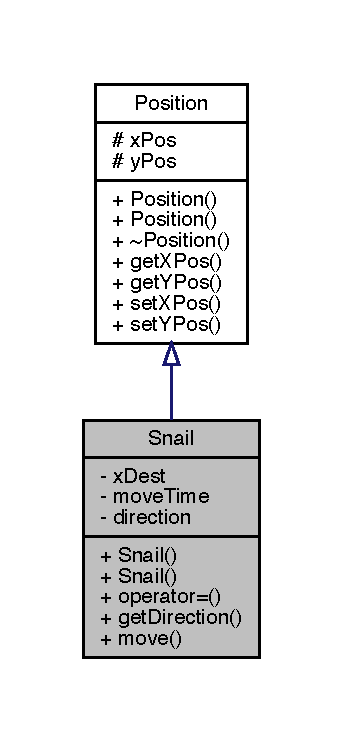
\includegraphics[width=165pt]{class_snail__inherit__graph}
\end{center}
\end{figure}


Collaboration diagram for Snail\+:
\nopagebreak
\begin{figure}[H]
\begin{center}
\leavevmode
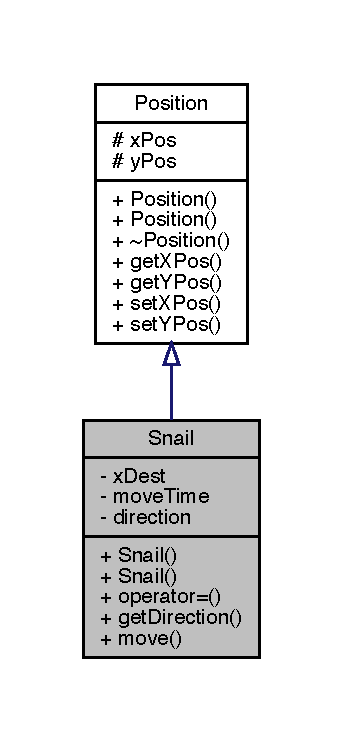
\includegraphics[width=165pt]{class_snail__coll__graph}
\end{center}
\end{figure}
\subsection*{Public Member Functions}
\begin{DoxyCompactItemize}
\item 
\mbox{\hyperlink{class_snail_ac5501ca7ead01b2ba0b7286503599f68}{Snail}} ()
\item 
\mbox{\hyperlink{class_snail_a89de76e5c6b4087c0ed7ac2809f0c45b}{Snail}} (double)
\item 
\mbox{\hyperlink{class_snail}{Snail}} \mbox{\hyperlink{class_snail_a107c53b3f7917e1b31134bf6064af32c}{operator=}} (const \mbox{\hyperlink{class_snail}{Snail}} \&S)
\item 
bool \mbox{\hyperlink{class_snail_a1cc5dc295038ac11f138ac49cdcfffc3}{get\+Direction}} () const
\item 
void \mbox{\hyperlink{class_snail_a7db73c2ca4146c04e7e37e444c15b08d}{move}} (double, double, bool)
\end{DoxyCompactItemize}
\subsection*{Private Attributes}
\begin{DoxyCompactItemize}
\item 
double \mbox{\hyperlink{class_snail_ab24202a09a2bfc54a801d963bab10a34}{x\+Dest}}
\item 
double \mbox{\hyperlink{class_snail_a16550c11e1c28bdd178cc0300436f054}{move\+Time}}
\item 
bool \mbox{\hyperlink{class_snail_aa0ebca6e0094ccfac4909f8f47323e2d}{direction}}
\end{DoxyCompactItemize}
\subsection*{Additional Inherited Members}


\subsection{Constructor \& Destructor Documentation}
\mbox{\Hypertarget{class_snail_ac5501ca7ead01b2ba0b7286503599f68}\label{class_snail_ac5501ca7ead01b2ba0b7286503599f68}} 
\index{Snail@{Snail}!Snail@{Snail}}
\index{Snail@{Snail}!Snail@{Snail}}
\subsubsection{\texorpdfstring{Snail()}{Snail()}\hspace{0.1cm}{\footnotesize\ttfamily [1/2]}}
{\footnotesize\ttfamily Snail\+::\+Snail (\begin{DoxyParamCaption}{ }\end{DoxyParamCaption})}

\mbox{\Hypertarget{class_snail_a89de76e5c6b4087c0ed7ac2809f0c45b}\label{class_snail_a89de76e5c6b4087c0ed7ac2809f0c45b}} 
\index{Snail@{Snail}!Snail@{Snail}}
\index{Snail@{Snail}!Snail@{Snail}}
\subsubsection{\texorpdfstring{Snail()}{Snail()}\hspace{0.1cm}{\footnotesize\ttfamily [2/2]}}
{\footnotesize\ttfamily Snail\+::\+Snail (\begin{DoxyParamCaption}\item[{double}]{\+\_\+xpos }\end{DoxyParamCaption})}



\subsection{Member Function Documentation}
\mbox{\Hypertarget{class_snail_a1cc5dc295038ac11f138ac49cdcfffc3}\label{class_snail_a1cc5dc295038ac11f138ac49cdcfffc3}} 
\index{Snail@{Snail}!get\+Direction@{get\+Direction}}
\index{get\+Direction@{get\+Direction}!Snail@{Snail}}
\subsubsection{\texorpdfstring{get\+Direction()}{getDirection()}}
{\footnotesize\ttfamily bool Snail\+::get\+Direction (\begin{DoxyParamCaption}{ }\end{DoxyParamCaption}) const}

\mbox{\Hypertarget{class_snail_a7db73c2ca4146c04e7e37e444c15b08d}\label{class_snail_a7db73c2ca4146c04e7e37e444c15b08d}} 
\index{Snail@{Snail}!move@{move}}
\index{move@{move}!Snail@{Snail}}
\subsubsection{\texorpdfstring{move()}{move()}}
{\footnotesize\ttfamily void Snail\+::move (\begin{DoxyParamCaption}\item[{double}]{\+\_\+x,  }\item[{double}]{t,  }\item[{bool}]{huntcoin }\end{DoxyParamCaption})}

\mbox{\Hypertarget{class_snail_a107c53b3f7917e1b31134bf6064af32c}\label{class_snail_a107c53b3f7917e1b31134bf6064af32c}} 
\index{Snail@{Snail}!operator=@{operator=}}
\index{operator=@{operator=}!Snail@{Snail}}
\subsubsection{\texorpdfstring{operator=()}{operator=()}}
{\footnotesize\ttfamily \mbox{\hyperlink{class_snail}{Snail}} Snail\+::operator= (\begin{DoxyParamCaption}\item[{const \mbox{\hyperlink{class_snail}{Snail}} \&}]{S }\end{DoxyParamCaption})}

Here is the call graph for this function\+:
\nopagebreak
\begin{figure}[H]
\begin{center}
\leavevmode
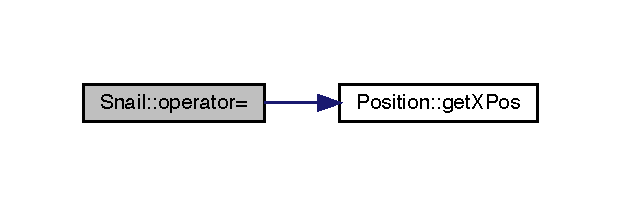
\includegraphics[width=298pt]{class_snail_a107c53b3f7917e1b31134bf6064af32c_cgraph}
\end{center}
\end{figure}


\subsection{Member Data Documentation}
\mbox{\Hypertarget{class_snail_aa0ebca6e0094ccfac4909f8f47323e2d}\label{class_snail_aa0ebca6e0094ccfac4909f8f47323e2d}} 
\index{Snail@{Snail}!direction@{direction}}
\index{direction@{direction}!Snail@{Snail}}
\subsubsection{\texorpdfstring{direction}{direction}}
{\footnotesize\ttfamily bool Snail\+::direction\hspace{0.3cm}{\ttfamily [private]}}

\mbox{\Hypertarget{class_snail_a16550c11e1c28bdd178cc0300436f054}\label{class_snail_a16550c11e1c28bdd178cc0300436f054}} 
\index{Snail@{Snail}!move\+Time@{move\+Time}}
\index{move\+Time@{move\+Time}!Snail@{Snail}}
\subsubsection{\texorpdfstring{move\+Time}{moveTime}}
{\footnotesize\ttfamily double Snail\+::move\+Time\hspace{0.3cm}{\ttfamily [private]}}

\mbox{\Hypertarget{class_snail_ab24202a09a2bfc54a801d963bab10a34}\label{class_snail_ab24202a09a2bfc54a801d963bab10a34}} 
\index{Snail@{Snail}!x\+Dest@{x\+Dest}}
\index{x\+Dest@{x\+Dest}!Snail@{Snail}}
\subsubsection{\texorpdfstring{x\+Dest}{xDest}}
{\footnotesize\ttfamily double Snail\+::x\+Dest\hspace{0.3cm}{\ttfamily [private]}}



The documentation for this class was generated from the following files\+:\begin{DoxyCompactItemize}
\item 
\mbox{\hyperlink{_snail_8hpp}{Snail.\+hpp}}\item 
\mbox{\hyperlink{_snail_8cpp}{Snail.\+cpp}}\end{DoxyCompactItemize}

\chapter{File Documentation}
\hypertarget{_aquarium_8cpp}{}\section{Aquarium.\+cpp File Reference}
\label{_aquarium_8cpp}\index{Aquarium.\+cpp@{Aquarium.\+cpp}}
{\ttfamily \#include \char`\"{}Aquarium.\+hpp\char`\"{}}\newline
{\ttfamily \#include $<$iostream$>$}\newline
Include dependency graph for Aquarium.\+cpp\+:
\nopagebreak
\begin{figure}[H]
\begin{center}
\leavevmode
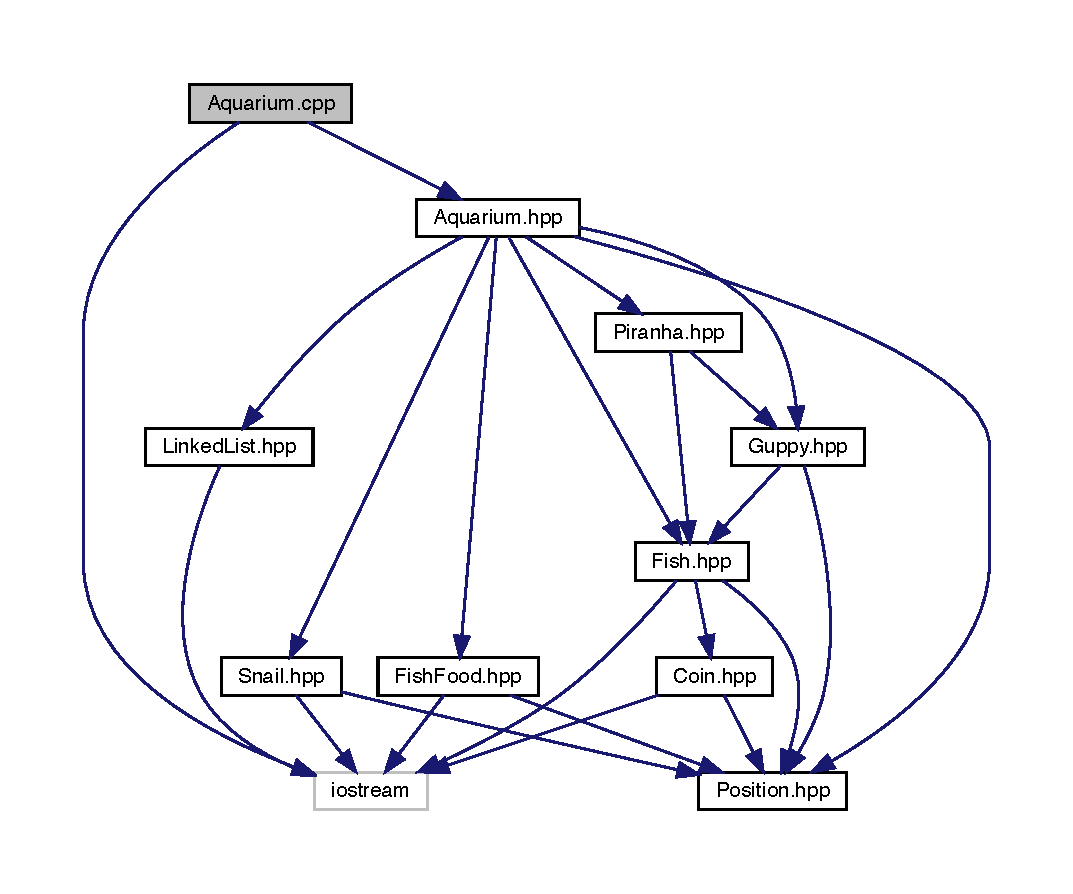
\includegraphics[width=350pt]{_aquarium_8cpp__incl}
\end{center}
\end{figure}

\hypertarget{_aquarium_8hpp}{}\section{Aquarium.\+hpp File Reference}
\label{_aquarium_8hpp}\index{Aquarium.\+hpp@{Aquarium.\+hpp}}
{\ttfamily \#include \char`\"{}Linked\+List.\+hpp\char`\"{}}\newline
{\ttfamily \#include \char`\"{}Fish.\+hpp\char`\"{}}\newline
{\ttfamily \#include \char`\"{}Snail.\+hpp\char`\"{}}\newline
{\ttfamily \#include \char`\"{}Piranha.\+hpp\char`\"{}}\newline
{\ttfamily \#include \char`\"{}Guppy.\+hpp\char`\"{}}\newline
{\ttfamily \#include \char`\"{}Fish\+Food.\+hpp\char`\"{}}\newline
{\ttfamily \#include \char`\"{}Position.\+hpp\char`\"{}}\newline
Include dependency graph for Aquarium.\+hpp\+:
\nopagebreak
\begin{figure}[H]
\begin{center}
\leavevmode
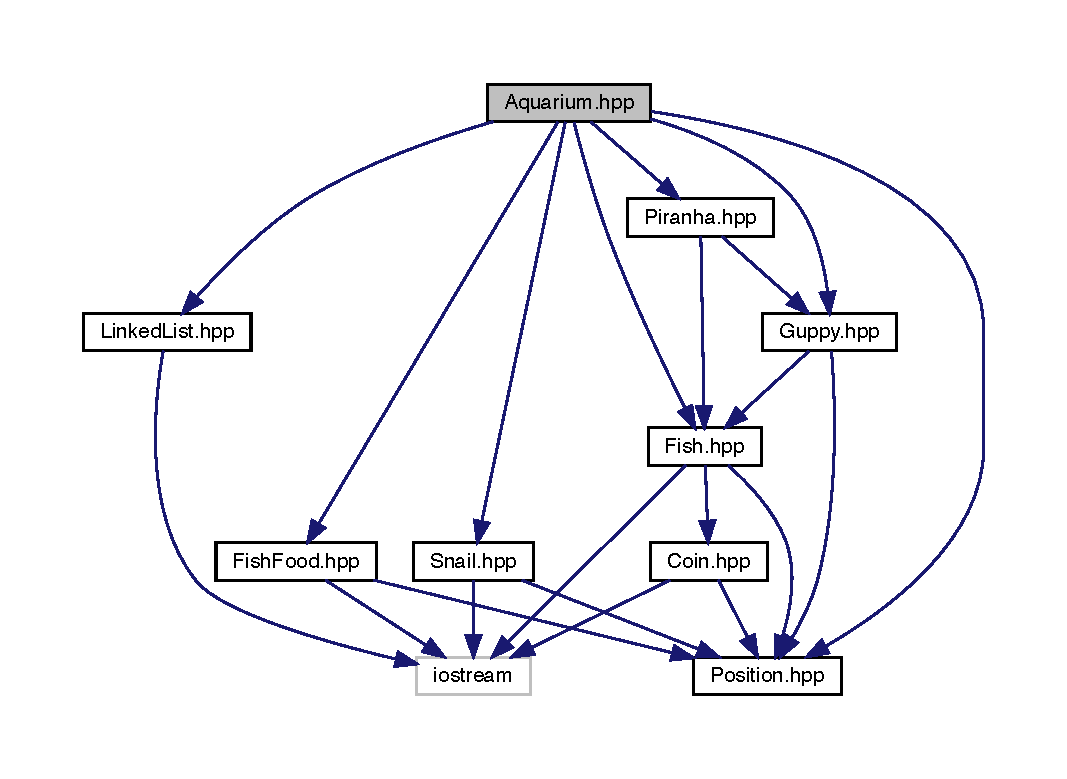
\includegraphics[width=350pt]{_aquarium_8hpp__incl}
\end{center}
\end{figure}
This graph shows which files directly or indirectly include this file\+:
\nopagebreak
\begin{figure}[H]
\begin{center}
\leavevmode
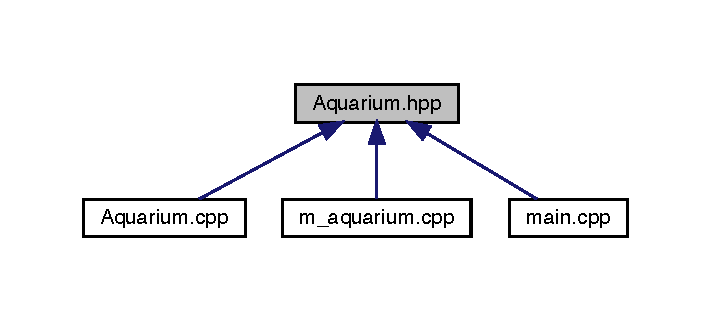
\includegraphics[width=341pt]{_aquarium_8hpp__dep__incl}
\end{center}
\end{figure}
\subsection*{Classes}
\begin{DoxyCompactItemize}
\item 
class \mbox{\hyperlink{class_aquarium}{Aquarium}}
\end{DoxyCompactItemize}

\hypertarget{_coin_8cpp}{}\section{Coin.\+cpp File Reference}
\label{_coin_8cpp}\index{Coin.\+cpp@{Coin.\+cpp}}
{\ttfamily \#include \char`\"{}Coin.\+hpp\char`\"{}}\newline
Include dependency graph for Coin.\+cpp\+:
\nopagebreak
\begin{figure}[H]
\begin{center}
\leavevmode
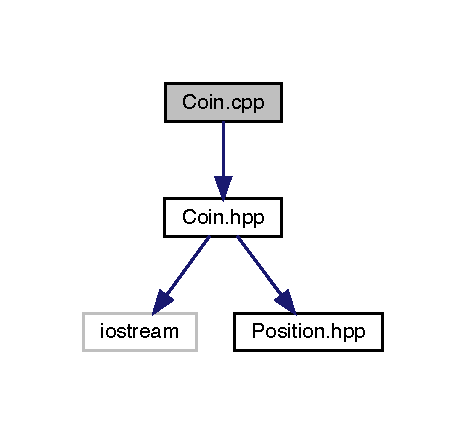
\includegraphics[width=224pt]{_coin_8cpp__incl}
\end{center}
\end{figure}

\hypertarget{_coin_8hpp}{}\section{Coin.\+hpp File Reference}
\label{_coin_8hpp}\index{Coin.\+hpp@{Coin.\+hpp}}
{\ttfamily \#include $<$iostream$>$}\newline
{\ttfamily \#include \char`\"{}Position.\+hpp\char`\"{}}\newline
Include dependency graph for Coin.\+hpp\+:
\nopagebreak
\begin{figure}[H]
\begin{center}
\leavevmode
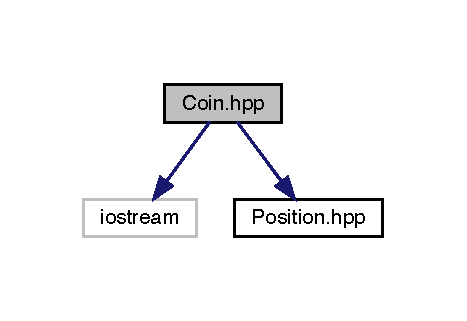
\includegraphics[width=224pt]{_coin_8hpp__incl}
\end{center}
\end{figure}
This graph shows which files directly or indirectly include this file\+:
\nopagebreak
\begin{figure}[H]
\begin{center}
\leavevmode
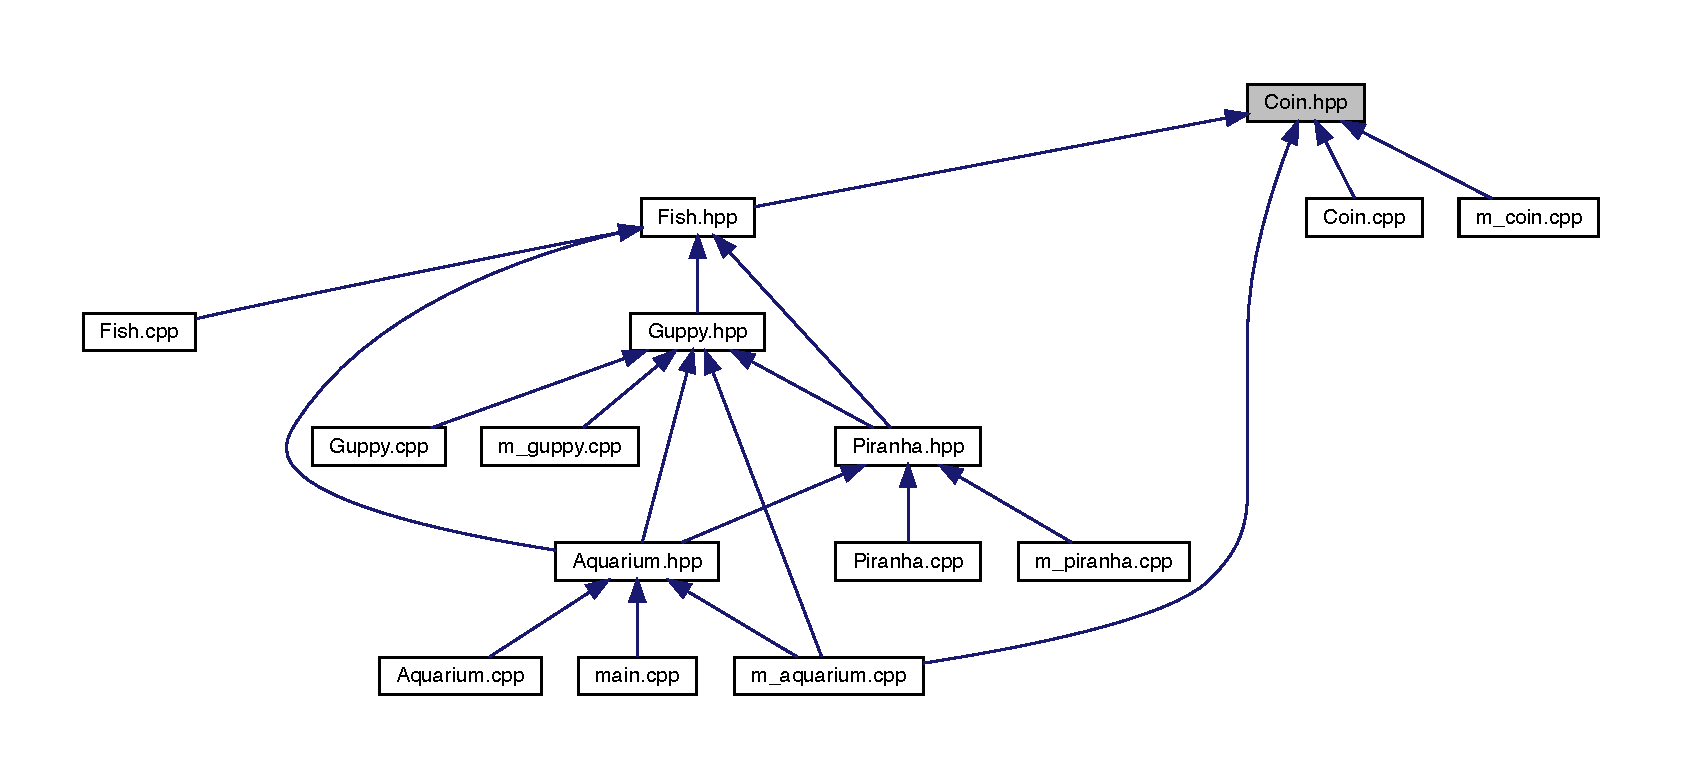
\includegraphics[width=350pt]{_coin_8hpp__dep__incl}
\end{center}
\end{figure}
\subsection*{Classes}
\begin{DoxyCompactItemize}
\item 
class \mbox{\hyperlink{class_coin}{Coin}}
\end{DoxyCompactItemize}

\hypertarget{_fish_8cpp}{}\section{Fish.\+cpp File Reference}
\label{_fish_8cpp}\index{Fish.\+cpp@{Fish.\+cpp}}
{\ttfamily \#include \char`\"{}Fish.\+hpp\char`\"{}}\newline
{\ttfamily \#include $<$cstdlib$>$}\newline
{\ttfamily \#include $<$cmath$>$}\newline
Include dependency graph for Fish.\+cpp\+:
\nopagebreak
\begin{figure}[H]
\begin{center}
\leavevmode
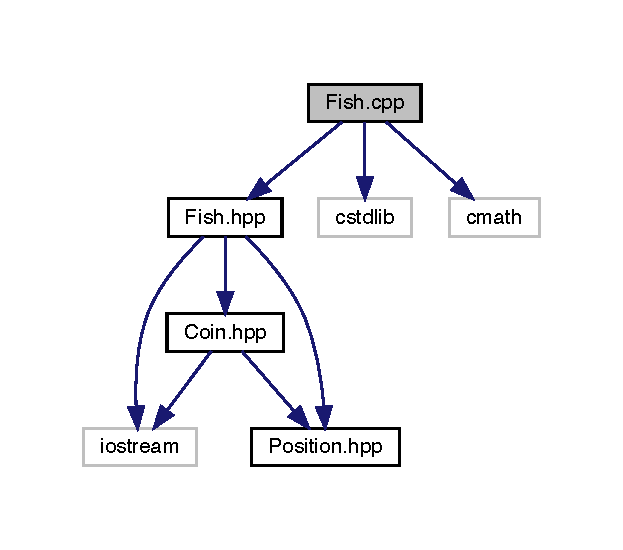
\includegraphics[width=299pt]{_fish_8cpp__incl}
\end{center}
\end{figure}
\subsection*{Variables}
\begin{DoxyCompactItemize}
\item 
const int \mbox{\hyperlink{_fish_8cpp_a3482785bd2a4c8b307f9e0b6f54e2c36}{S\+C\+R\+E\+E\+N\+\_\+\+W\+I\+D\+TH}} = 640
\item 
const int \mbox{\hyperlink{_fish_8cpp_ab454541ae58bcf6555e8d723b1eb95e7}{S\+C\+R\+E\+E\+N\+\_\+\+H\+E\+I\+G\+HT}} = 480
\end{DoxyCompactItemize}


\subsection{Variable Documentation}
\mbox{\Hypertarget{_fish_8cpp_ab454541ae58bcf6555e8d723b1eb95e7}\label{_fish_8cpp_ab454541ae58bcf6555e8d723b1eb95e7}} 
\index{Fish.\+cpp@{Fish.\+cpp}!S\+C\+R\+E\+E\+N\+\_\+\+H\+E\+I\+G\+HT@{S\+C\+R\+E\+E\+N\+\_\+\+H\+E\+I\+G\+HT}}
\index{S\+C\+R\+E\+E\+N\+\_\+\+H\+E\+I\+G\+HT@{S\+C\+R\+E\+E\+N\+\_\+\+H\+E\+I\+G\+HT}!Fish.\+cpp@{Fish.\+cpp}}
\subsubsection{\texorpdfstring{S\+C\+R\+E\+E\+N\+\_\+\+H\+E\+I\+G\+HT}{SCREEN\_HEIGHT}}
{\footnotesize\ttfamily const int S\+C\+R\+E\+E\+N\+\_\+\+H\+E\+I\+G\+HT = 480}

\mbox{\Hypertarget{_fish_8cpp_a3482785bd2a4c8b307f9e0b6f54e2c36}\label{_fish_8cpp_a3482785bd2a4c8b307f9e0b6f54e2c36}} 
\index{Fish.\+cpp@{Fish.\+cpp}!S\+C\+R\+E\+E\+N\+\_\+\+W\+I\+D\+TH@{S\+C\+R\+E\+E\+N\+\_\+\+W\+I\+D\+TH}}
\index{S\+C\+R\+E\+E\+N\+\_\+\+W\+I\+D\+TH@{S\+C\+R\+E\+E\+N\+\_\+\+W\+I\+D\+TH}!Fish.\+cpp@{Fish.\+cpp}}
\subsubsection{\texorpdfstring{S\+C\+R\+E\+E\+N\+\_\+\+W\+I\+D\+TH}{SCREEN\_WIDTH}}
{\footnotesize\ttfamily const int S\+C\+R\+E\+E\+N\+\_\+\+W\+I\+D\+TH = 640}


\hypertarget{_fish_8hpp}{}\section{Fish.\+hpp File Reference}
\label{_fish_8hpp}\index{Fish.\+hpp@{Fish.\+hpp}}
{\ttfamily \#include $<$iostream$>$}\newline
{\ttfamily \#include \char`\"{}Coin.\+hpp\char`\"{}}\newline
{\ttfamily \#include \char`\"{}Position.\+hpp\char`\"{}}\newline
Include dependency graph for Fish.\+hpp\+:
\nopagebreak
\begin{figure}[H]
\begin{center}
\leavevmode
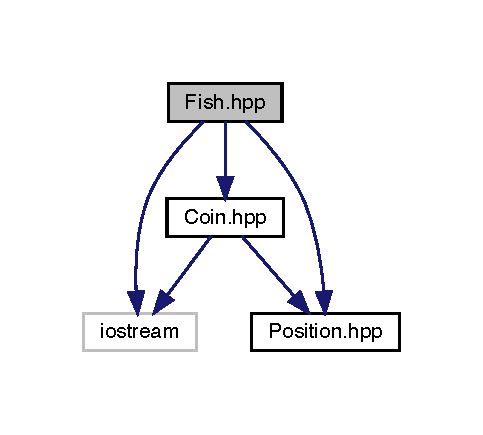
\includegraphics[width=232pt]{_fish_8hpp__incl}
\end{center}
\end{figure}
This graph shows which files directly or indirectly include this file\+:
\nopagebreak
\begin{figure}[H]
\begin{center}
\leavevmode
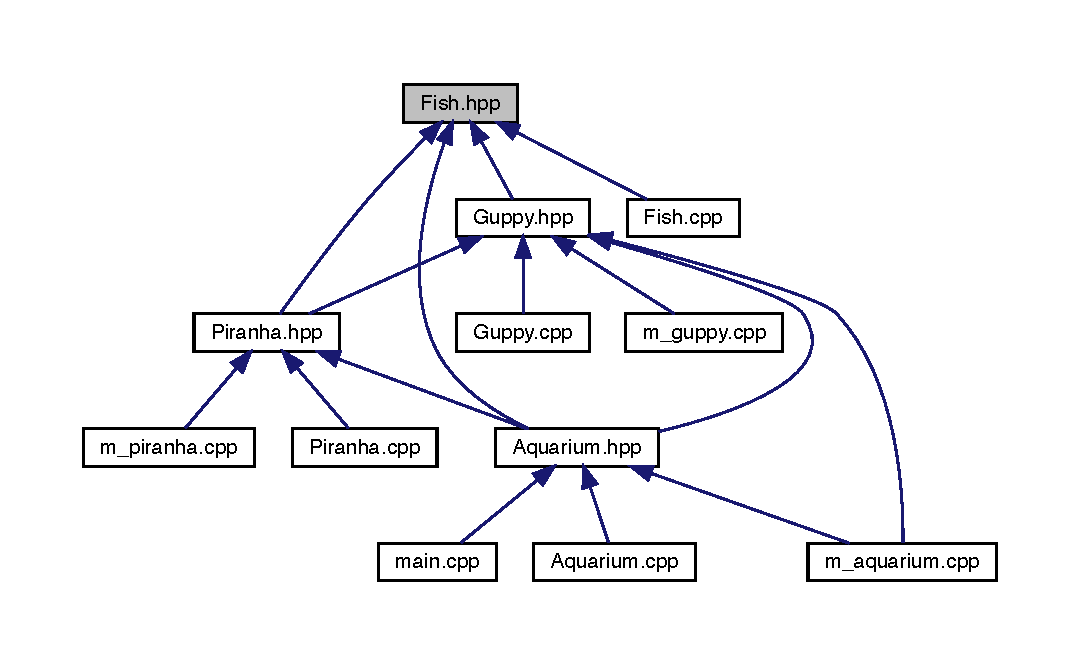
\includegraphics[width=350pt]{_fish_8hpp__dep__incl}
\end{center}
\end{figure}
\subsection*{Classes}
\begin{DoxyCompactItemize}
\item 
class \mbox{\hyperlink{class_fish}{Fish}}
\end{DoxyCompactItemize}

\hypertarget{_fish_food_8cpp}{}\section{Fish\+Food.\+cpp File Reference}
\label{_fish_food_8cpp}\index{Fish\+Food.\+cpp@{Fish\+Food.\+cpp}}
{\ttfamily \#include \char`\"{}Fish\+Food.\+hpp\char`\"{}}\newline
Include dependency graph for Fish\+Food.\+cpp\+:
\nopagebreak
\begin{figure}[H]
\begin{center}
\leavevmode
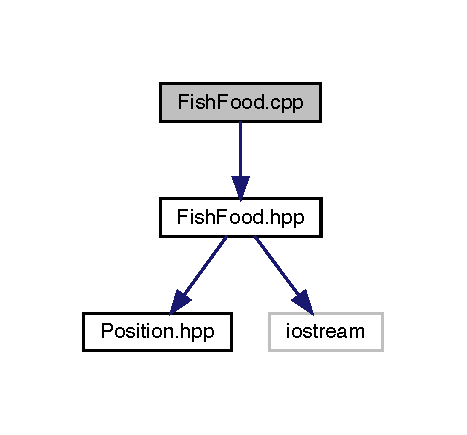
\includegraphics[width=224pt]{_fish_food_8cpp__incl}
\end{center}
\end{figure}

\hypertarget{_fish_food_8hpp}{}\section{Fish\+Food.\+hpp File Reference}
\label{_fish_food_8hpp}\index{Fish\+Food.\+hpp@{Fish\+Food.\+hpp}}
{\ttfamily \#include \char`\"{}Position.\+hpp\char`\"{}}\newline
{\ttfamily \#include $<$iostream$>$}\newline
Include dependency graph for Fish\+Food.\+hpp\+:
\nopagebreak
\begin{figure}[H]
\begin{center}
\leavevmode
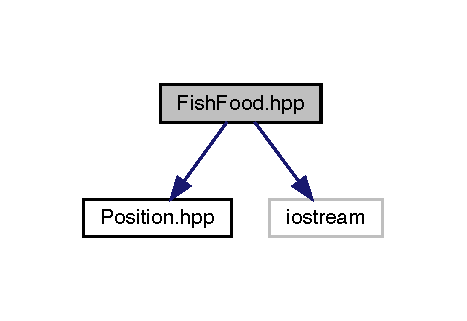
\includegraphics[width=224pt]{_fish_food_8hpp__incl}
\end{center}
\end{figure}
This graph shows which files directly or indirectly include this file\+:
\nopagebreak
\begin{figure}[H]
\begin{center}
\leavevmode
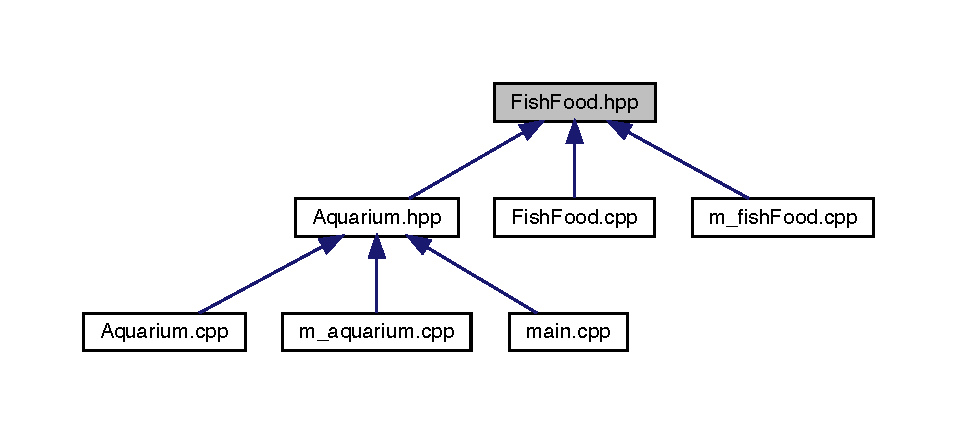
\includegraphics[width=350pt]{_fish_food_8hpp__dep__incl}
\end{center}
\end{figure}
\subsection*{Classes}
\begin{DoxyCompactItemize}
\item 
class \mbox{\hyperlink{class_fish_food}{Fish\+Food}}
\end{DoxyCompactItemize}

\hypertarget{_guppy_8cpp}{}\section{Guppy.\+cpp File Reference}
\label{_guppy_8cpp}\index{Guppy.\+cpp@{Guppy.\+cpp}}
{\ttfamily \#include \char`\"{}Guppy.\+hpp\char`\"{}}\newline
Include dependency graph for Guppy.\+cpp\+:
\nopagebreak
\begin{figure}[H]
\begin{center}
\leavevmode
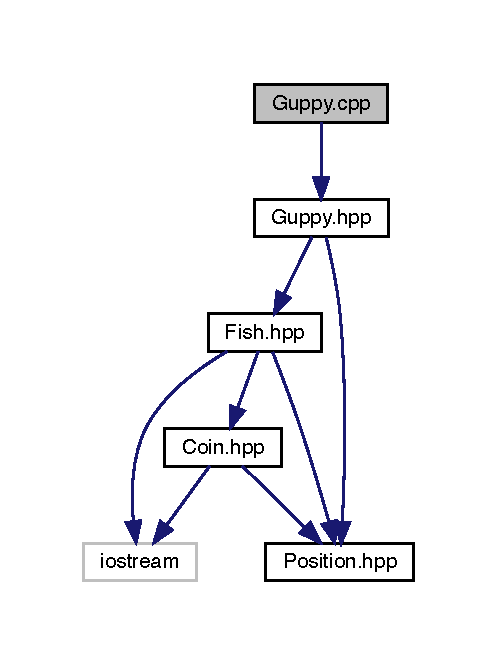
\includegraphics[width=239pt]{_guppy_8cpp__incl}
\end{center}
\end{figure}

\hypertarget{_guppy_8hpp}{}\section{Guppy.\+hpp File Reference}
\label{_guppy_8hpp}\index{Guppy.\+hpp@{Guppy.\+hpp}}
{\ttfamily \#include \char`\"{}Fish.\+hpp\char`\"{}}\newline
{\ttfamily \#include \char`\"{}Position.\+hpp\char`\"{}}\newline
Include dependency graph for Guppy.\+hpp\+:
\nopagebreak
\begin{figure}[H]
\begin{center}
\leavevmode
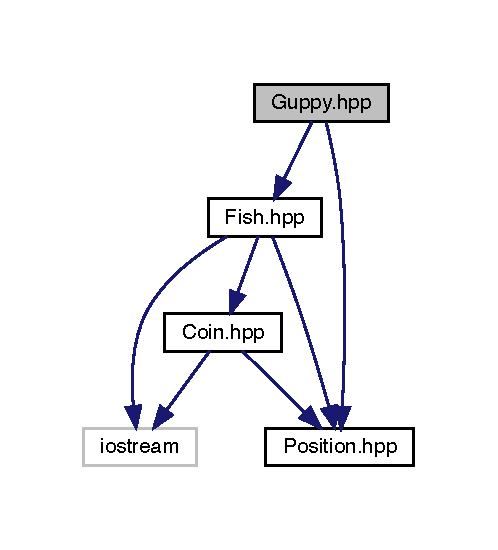
\includegraphics[width=239pt]{_guppy_8hpp__incl}
\end{center}
\end{figure}
This graph shows which files directly or indirectly include this file\+:
\nopagebreak
\begin{figure}[H]
\begin{center}
\leavevmode
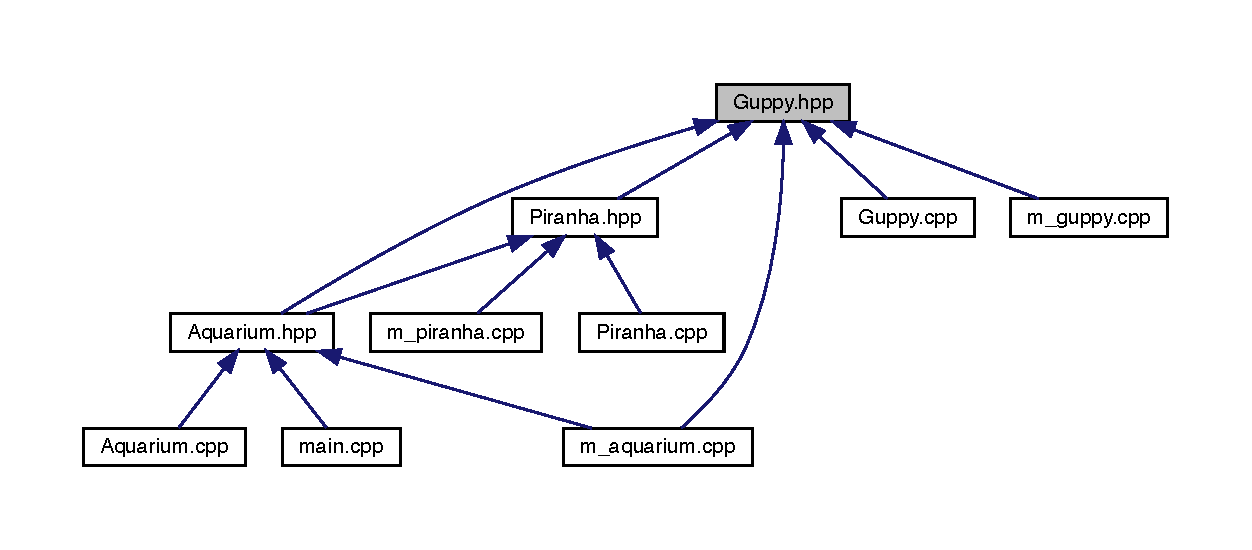
\includegraphics[width=350pt]{_guppy_8hpp__dep__incl}
\end{center}
\end{figure}
\subsection*{Classes}
\begin{DoxyCompactItemize}
\item 
class \mbox{\hyperlink{class_guppy}{Guppy}}
\end{DoxyCompactItemize}

\hypertarget{_linked_list_8hpp}{}\section{Linked\+List.\+hpp File Reference}
\label{_linked_list_8hpp}\index{Linked\+List.\+hpp@{Linked\+List.\+hpp}}
{\ttfamily \#include $<$iostream$>$}\newline
Include dependency graph for Linked\+List.\+hpp\+:
\nopagebreak
\begin{figure}[H]
\begin{center}
\leavevmode
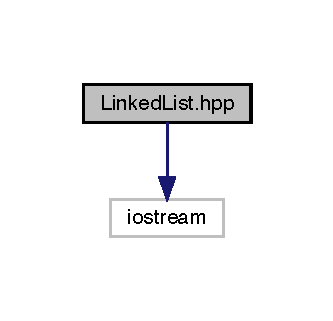
\includegraphics[width=160pt]{_linked_list_8hpp__incl}
\end{center}
\end{figure}
This graph shows which files directly or indirectly include this file\+:
\nopagebreak
\begin{figure}[H]
\begin{center}
\leavevmode
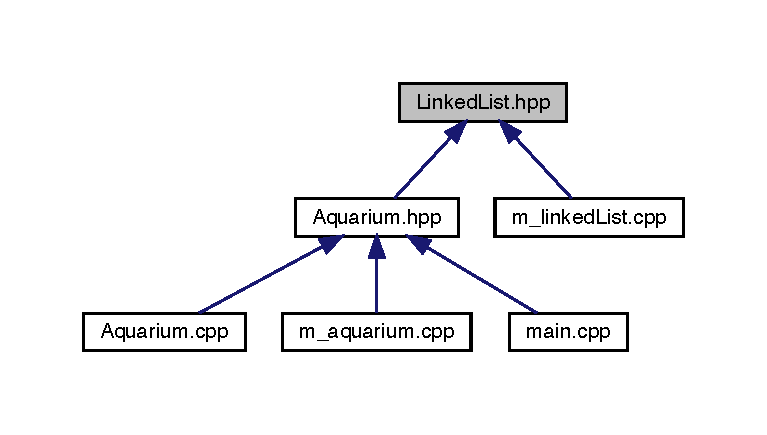
\includegraphics[width=350pt]{_linked_list_8hpp__dep__incl}
\end{center}
\end{figure}
\subsection*{Classes}
\begin{DoxyCompactItemize}
\item 
struct \mbox{\hyperlink{structnode}{node$<$ T $>$}}
\item 
class \mbox{\hyperlink{class_linked_list}{Linked\+List$<$ T $>$}}
\end{DoxyCompactItemize}

\hypertarget{m__aquarium_8cpp}{}\section{m\+\_\+aquarium.\+cpp File Reference}
\label{m__aquarium_8cpp}\index{m\+\_\+aquarium.\+cpp@{m\+\_\+aquarium.\+cpp}}
{\ttfamily \#include \char`\"{}Aquarium.\+hpp\char`\"{}}\newline
{\ttfamily \#include \char`\"{}Guppy.\+hpp\char`\"{}}\newline
{\ttfamily \#include \char`\"{}Snail.\+hpp\char`\"{}}\newline
{\ttfamily \#include \char`\"{}Coin.\+hpp\char`\"{}}\newline
{\ttfamily \#include $<$iostream$>$}\newline
Include dependency graph for m\+\_\+aquarium.\+cpp\+:
\nopagebreak
\begin{figure}[H]
\begin{center}
\leavevmode
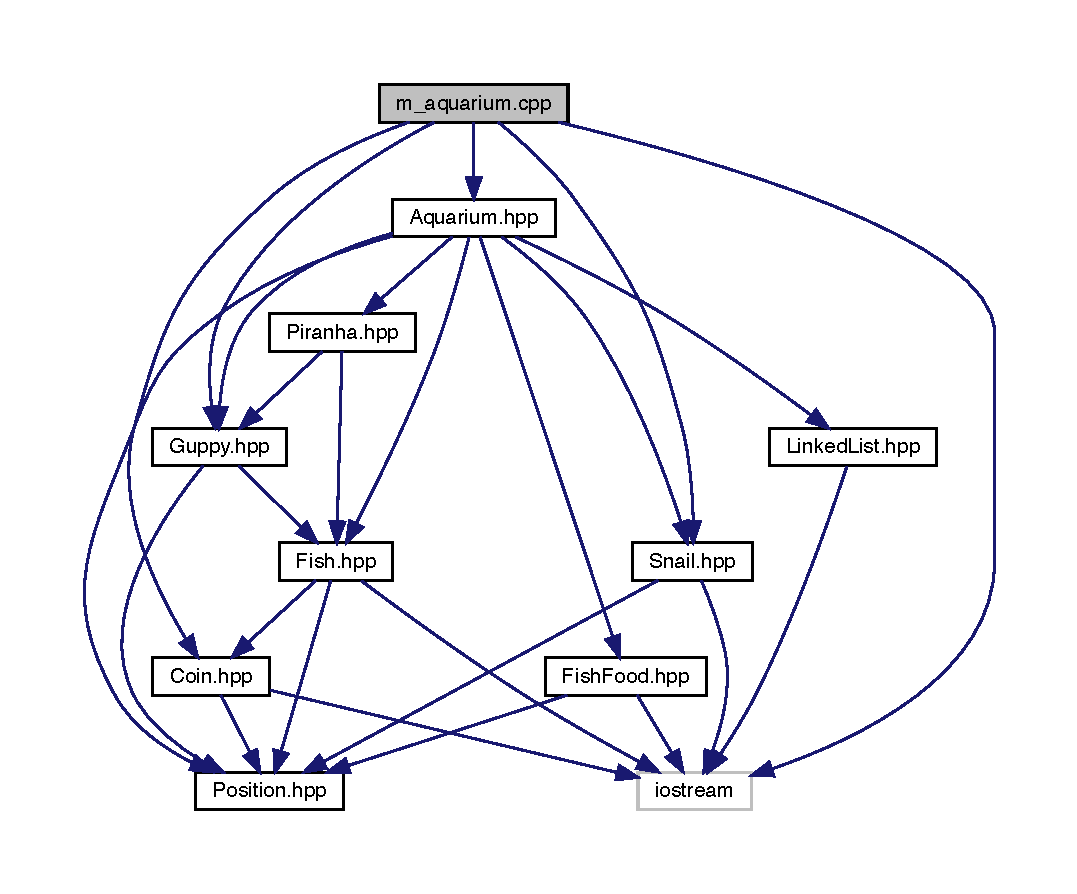
\includegraphics[width=350pt]{m__aquarium_8cpp__incl}
\end{center}
\end{figure}
\subsection*{Functions}
\begin{DoxyCompactItemize}
\item 
int \mbox{\hyperlink{m__aquarium_8cpp_ae66f6b31b5ad750f1fe042a706a4e3d4}{main}} ()
\end{DoxyCompactItemize}


\subsection{Function Documentation}
\mbox{\Hypertarget{m__aquarium_8cpp_ae66f6b31b5ad750f1fe042a706a4e3d4}\label{m__aquarium_8cpp_ae66f6b31b5ad750f1fe042a706a4e3d4}} 
\index{m\+\_\+aquarium.\+cpp@{m\+\_\+aquarium.\+cpp}!main@{main}}
\index{main@{main}!m\+\_\+aquarium.\+cpp@{m\+\_\+aquarium.\+cpp}}
\subsubsection{\texorpdfstring{main()}{main()}}
{\footnotesize\ttfamily int main (\begin{DoxyParamCaption}{ }\end{DoxyParamCaption})}

Here is the call graph for this function\+:
\nopagebreak
\begin{figure}[H]
\begin{center}
\leavevmode
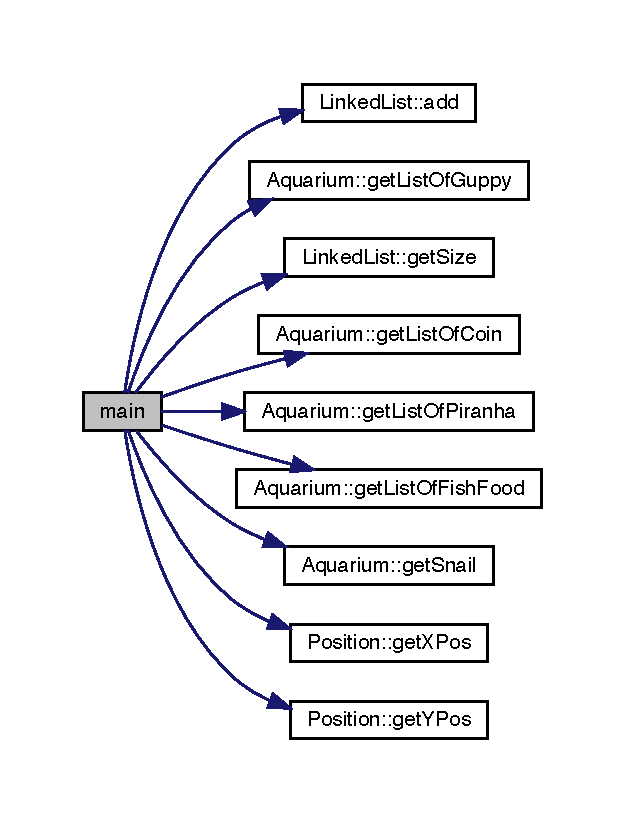
\includegraphics[width=300pt]{m__aquarium_8cpp_ae66f6b31b5ad750f1fe042a706a4e3d4_cgraph}
\end{center}
\end{figure}

\hypertarget{m__coin_8cpp}{}\section{m\+\_\+coin.\+cpp File Reference}
\label{m__coin_8cpp}\index{m\+\_\+coin.\+cpp@{m\+\_\+coin.\+cpp}}
{\ttfamily \#include \char`\"{}Coin.\+hpp\char`\"{}}\newline
{\ttfamily \#include $<$iostream$>$}\newline
Include dependency graph for m\+\_\+coin.\+cpp\+:
\nopagebreak
\begin{figure}[H]
\begin{center}
\leavevmode
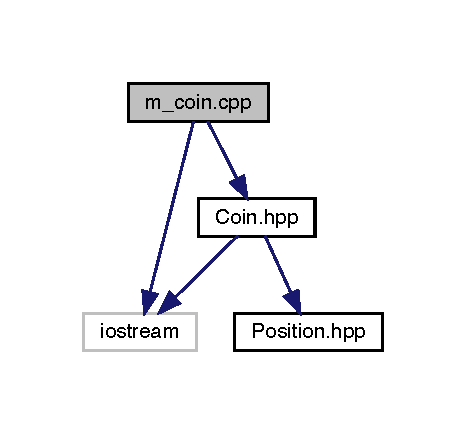
\includegraphics[width=224pt]{m__coin_8cpp__incl}
\end{center}
\end{figure}
\subsection*{Functions}
\begin{DoxyCompactItemize}
\item 
int \mbox{\hyperlink{m__coin_8cpp_ae66f6b31b5ad750f1fe042a706a4e3d4}{main}} ()
\end{DoxyCompactItemize}


\subsection{Function Documentation}
\mbox{\Hypertarget{m__coin_8cpp_ae66f6b31b5ad750f1fe042a706a4e3d4}\label{m__coin_8cpp_ae66f6b31b5ad750f1fe042a706a4e3d4}} 
\index{m\+\_\+coin.\+cpp@{m\+\_\+coin.\+cpp}!main@{main}}
\index{main@{main}!m\+\_\+coin.\+cpp@{m\+\_\+coin.\+cpp}}
\subsubsection{\texorpdfstring{main()}{main()}}
{\footnotesize\ttfamily int main (\begin{DoxyParamCaption}{ }\end{DoxyParamCaption})}

Here is the call graph for this function\+:
\nopagebreak
\begin{figure}[H]
\begin{center}
\leavevmode
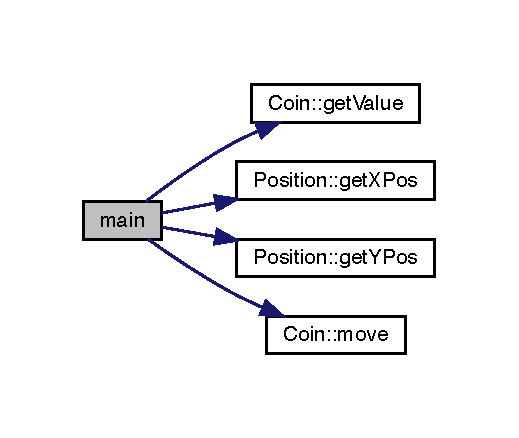
\includegraphics[width=249pt]{m__coin_8cpp_ae66f6b31b5ad750f1fe042a706a4e3d4_cgraph}
\end{center}
\end{figure}

\hypertarget{m__fish_food_8cpp}{}\section{m\+\_\+fish\+Food.\+cpp File Reference}
\label{m__fish_food_8cpp}\index{m\+\_\+fish\+Food.\+cpp@{m\+\_\+fish\+Food.\+cpp}}
{\ttfamily \#include \char`\"{}Fish\+Food.\+hpp\char`\"{}}\newline
{\ttfamily \#include $<$iostream$>$}\newline
Include dependency graph for m\+\_\+fish\+Food.\+cpp\+:
\nopagebreak
\begin{figure}[H]
\begin{center}
\leavevmode
\includegraphics[width=224pt]{m__fish_food_8cpp__incl}
\end{center}
\end{figure}
\subsection*{Functions}
\begin{DoxyCompactItemize}
\item 
int \mbox{\hyperlink{m__fish_food_8cpp_ae66f6b31b5ad750f1fe042a706a4e3d4}{main}} ()
\end{DoxyCompactItemize}


\subsection{Function Documentation}
\mbox{\Hypertarget{m__fish_food_8cpp_ae66f6b31b5ad750f1fe042a706a4e3d4}\label{m__fish_food_8cpp_ae66f6b31b5ad750f1fe042a706a4e3d4}} 
\index{m\+\_\+fish\+Food.\+cpp@{m\+\_\+fish\+Food.\+cpp}!main@{main}}
\index{main@{main}!m\+\_\+fish\+Food.\+cpp@{m\+\_\+fish\+Food.\+cpp}}
\subsubsection{\texorpdfstring{main()}{main()}}
{\footnotesize\ttfamily int main (\begin{DoxyParamCaption}{ }\end{DoxyParamCaption})}

Here is the call graph for this function\+:
\nopagebreak
\begin{figure}[H]
\begin{center}
\leavevmode
\includegraphics[width=249pt]{m__fish_food_8cpp_ae66f6b31b5ad750f1fe042a706a4e3d4_cgraph}
\end{center}
\end{figure}

\hypertarget{m__guppy_8cpp}{}\section{m\+\_\+guppy.\+cpp File Reference}
\label{m__guppy_8cpp}\index{m\+\_\+guppy.\+cpp@{m\+\_\+guppy.\+cpp}}
{\ttfamily \#include \char`\"{}Guppy.\+hpp\char`\"{}}\newline
{\ttfamily \#include $<$iostream$>$}\newline
Include dependency graph for m\+\_\+guppy.\+cpp\+:
\nopagebreak
\begin{figure}[H]
\begin{center}
\leavevmode
\includegraphics[width=256pt]{m__guppy_8cpp__incl}
\end{center}
\end{figure}
\subsection*{Functions}
\begin{DoxyCompactItemize}
\item 
int \mbox{\hyperlink{m__guppy_8cpp_ae66f6b31b5ad750f1fe042a706a4e3d4}{main}} ()
\end{DoxyCompactItemize}


\subsection{Function Documentation}
\mbox{\Hypertarget{m__guppy_8cpp_ae66f6b31b5ad750f1fe042a706a4e3d4}\label{m__guppy_8cpp_ae66f6b31b5ad750f1fe042a706a4e3d4}} 
\index{m\+\_\+guppy.\+cpp@{m\+\_\+guppy.\+cpp}!main@{main}}
\index{main@{main}!m\+\_\+guppy.\+cpp@{m\+\_\+guppy.\+cpp}}
\subsubsection{\texorpdfstring{main()}{main()}}
{\footnotesize\ttfamily int main (\begin{DoxyParamCaption}{ }\end{DoxyParamCaption})}

Here is the call graph for this function\+:
\nopagebreak
\begin{figure}[H]
\begin{center}
\leavevmode
\includegraphics[width=350pt]{m__guppy_8cpp_ae66f6b31b5ad750f1fe042a706a4e3d4_cgraph}
\end{center}
\end{figure}

\hypertarget{m__linked_list_8cpp}{}\section{m\+\_\+linked\+List.\+cpp File Reference}
\label{m__linked_list_8cpp}\index{m\+\_\+linked\+List.\+cpp@{m\+\_\+linked\+List.\+cpp}}
{\ttfamily \#include $<$iostream$>$}\newline
{\ttfamily \#include \char`\"{}Linked\+List.\+hpp\char`\"{}}\newline
Include dependency graph for m\+\_\+linked\+List.\+cpp\+:
\nopagebreak
\begin{figure}[H]
\begin{center}
\leavevmode
\includegraphics[width=199pt]{m__linked_list_8cpp__incl}
\end{center}
\end{figure}
\subsection*{Functions}
\begin{DoxyCompactItemize}
\item 
int \mbox{\hyperlink{m__linked_list_8cpp_ae66f6b31b5ad750f1fe042a706a4e3d4}{main}} ()
\end{DoxyCompactItemize}


\subsection{Function Documentation}
\mbox{\Hypertarget{m__linked_list_8cpp_ae66f6b31b5ad750f1fe042a706a4e3d4}\label{m__linked_list_8cpp_ae66f6b31b5ad750f1fe042a706a4e3d4}} 
\index{m\+\_\+linked\+List.\+cpp@{m\+\_\+linked\+List.\+cpp}!main@{main}}
\index{main@{main}!m\+\_\+linked\+List.\+cpp@{m\+\_\+linked\+List.\+cpp}}
\subsubsection{\texorpdfstring{main()}{main()}}
{\footnotesize\ttfamily int main (\begin{DoxyParamCaption}{ }\end{DoxyParamCaption})}

Here is the call graph for this function\+:
\nopagebreak
\begin{figure}[H]
\begin{center}
\leavevmode
\includegraphics[width=256pt]{m__linked_list_8cpp_ae66f6b31b5ad750f1fe042a706a4e3d4_cgraph}
\end{center}
\end{figure}

\hypertarget{m__piranha_8cpp}{}\section{m\+\_\+piranha.\+cpp File Reference}
\label{m__piranha_8cpp}\index{m\+\_\+piranha.\+cpp@{m\+\_\+piranha.\+cpp}}
{\ttfamily \#include \char`\"{}Piranha.\+hpp\char`\"{}}\newline
{\ttfamily \#include $<$iostream$>$}\newline
Include dependency graph for m\+\_\+piranha.\+cpp\+:
\nopagebreak
\begin{figure}[H]
\begin{center}
\leavevmode
\includegraphics[width=275pt]{m__piranha_8cpp__incl}
\end{center}
\end{figure}
\subsection*{Functions}
\begin{DoxyCompactItemize}
\item 
int \mbox{\hyperlink{m__piranha_8cpp_ae66f6b31b5ad750f1fe042a706a4e3d4}{main}} ()
\end{DoxyCompactItemize}


\subsection{Function Documentation}
\mbox{\Hypertarget{m__piranha_8cpp_ae66f6b31b5ad750f1fe042a706a4e3d4}\label{m__piranha_8cpp_ae66f6b31b5ad750f1fe042a706a4e3d4}} 
\index{m\+\_\+piranha.\+cpp@{m\+\_\+piranha.\+cpp}!main@{main}}
\index{main@{main}!m\+\_\+piranha.\+cpp@{m\+\_\+piranha.\+cpp}}
\subsubsection{\texorpdfstring{main()}{main()}}
{\footnotesize\ttfamily int main (\begin{DoxyParamCaption}{ }\end{DoxyParamCaption})}

Here is the call graph for this function\+:
\nopagebreak
\begin{figure}[H]
\begin{center}
\leavevmode
\includegraphics[width=350pt]{m__piranha_8cpp_ae66f6b31b5ad750f1fe042a706a4e3d4_cgraph}
\end{center}
\end{figure}

\hypertarget{m__position_8cpp}{}\section{m\+\_\+position.\+cpp File Reference}
\label{m__position_8cpp}\index{m\+\_\+position.\+cpp@{m\+\_\+position.\+cpp}}
{\ttfamily \#include \char`\"{}Position.\+hpp\char`\"{}}\newline
{\ttfamily \#include $<$iostream$>$}\newline
Include dependency graph for m\+\_\+position.\+cpp\+:
\nopagebreak
\begin{figure}[H]
\begin{center}
\leavevmode
\includegraphics[width=224pt]{m__position_8cpp__incl}
\end{center}
\end{figure}
\subsection*{Functions}
\begin{DoxyCompactItemize}
\item 
int \mbox{\hyperlink{m__position_8cpp_ae66f6b31b5ad750f1fe042a706a4e3d4}{main}} ()
\end{DoxyCompactItemize}


\subsection{Function Documentation}
\mbox{\Hypertarget{m__position_8cpp_ae66f6b31b5ad750f1fe042a706a4e3d4}\label{m__position_8cpp_ae66f6b31b5ad750f1fe042a706a4e3d4}} 
\index{m\+\_\+position.\+cpp@{m\+\_\+position.\+cpp}!main@{main}}
\index{main@{main}!m\+\_\+position.\+cpp@{m\+\_\+position.\+cpp}}
\subsubsection{\texorpdfstring{main()}{main()}}
{\footnotesize\ttfamily int main (\begin{DoxyParamCaption}{ }\end{DoxyParamCaption})}


\hypertarget{m__snail_8cpp}{}\section{m\+\_\+snail.\+cpp File Reference}
\label{m__snail_8cpp}\index{m\+\_\+snail.\+cpp@{m\+\_\+snail.\+cpp}}
{\ttfamily \#include \char`\"{}Snail.\+hpp\char`\"{}}\newline
{\ttfamily \#include $<$iostream$>$}\newline
Include dependency graph for m\+\_\+snail.\+cpp\+:
\nopagebreak
\begin{figure}[H]
\begin{center}
\leavevmode
\includegraphics[width=224pt]{m__snail_8cpp__incl}
\end{center}
\end{figure}
\subsection*{Functions}
\begin{DoxyCompactItemize}
\item 
int \mbox{\hyperlink{m__snail_8cpp_ae66f6b31b5ad750f1fe042a706a4e3d4}{main}} ()
\end{DoxyCompactItemize}


\subsection{Function Documentation}
\mbox{\Hypertarget{m__snail_8cpp_ae66f6b31b5ad750f1fe042a706a4e3d4}\label{m__snail_8cpp_ae66f6b31b5ad750f1fe042a706a4e3d4}} 
\index{m\+\_\+snail.\+cpp@{m\+\_\+snail.\+cpp}!main@{main}}
\index{main@{main}!m\+\_\+snail.\+cpp@{m\+\_\+snail.\+cpp}}
\subsubsection{\texorpdfstring{main()}{main()}}
{\footnotesize\ttfamily int main (\begin{DoxyParamCaption}{ }\end{DoxyParamCaption})}

Here is the call graph for this function\+:
\nopagebreak
\begin{figure}[H]
\begin{center}
\leavevmode
\includegraphics[width=251pt]{m__snail_8cpp_ae66f6b31b5ad750f1fe042a706a4e3d4_cgraph}
\end{center}
\end{figure}

\hypertarget{main_8cpp}{}\section{main.\+cpp File Reference}
\label{main_8cpp}\index{main.\+cpp@{main.\+cpp}}
{\ttfamily \#include \char`\"{}oop.\+hpp\char`\"{}}\newline
{\ttfamily \#include $<$iostream$>$}\newline
{\ttfamily \#include $<$math.\+h$>$}\newline
{\ttfamily \#include $<$sstream$>$}\newline
{\ttfamily \#include \char`\"{}Aquarium.\+hpp\char`\"{}}\newline
Include dependency graph for main.\+cpp\+:
\nopagebreak
\begin{figure}[H]
\begin{center}
\leavevmode
\includegraphics[width=350pt]{main_8cpp__incl}
\end{center}
\end{figure}
\subsection*{Functions}
\begin{DoxyCompactItemize}
\item 
double \mbox{\hyperlink{main_8cpp_ae56cd41b4527edcd0a196c2e2457f498}{calculate\+Distance}} (double x1, double y1, double x2, double y2)
\item 
int \mbox{\hyperlink{main_8cpp_a700a0caa5b70a06d1064e576f9f3cf65}{main}} (int argc, char $\ast$args\mbox{[}$\,$\mbox{]})
\end{DoxyCompactItemize}


\subsection{Function Documentation}
\mbox{\Hypertarget{main_8cpp_ae56cd41b4527edcd0a196c2e2457f498}\label{main_8cpp_ae56cd41b4527edcd0a196c2e2457f498}} 
\index{main.\+cpp@{main.\+cpp}!calculate\+Distance@{calculate\+Distance}}
\index{calculate\+Distance@{calculate\+Distance}!main.\+cpp@{main.\+cpp}}
\subsubsection{\texorpdfstring{calculate\+Distance()}{calculateDistance()}}
{\footnotesize\ttfamily double calculate\+Distance (\begin{DoxyParamCaption}\item[{double}]{x1,  }\item[{double}]{y1,  }\item[{double}]{x2,  }\item[{double}]{y2 }\end{DoxyParamCaption})}

\mbox{\Hypertarget{main_8cpp_a700a0caa5b70a06d1064e576f9f3cf65}\label{main_8cpp_a700a0caa5b70a06d1064e576f9f3cf65}} 
\index{main.\+cpp@{main.\+cpp}!main@{main}}
\index{main@{main}!main.\+cpp@{main.\+cpp}}
\subsubsection{\texorpdfstring{main()}{main()}}
{\footnotesize\ttfamily int main (\begin{DoxyParamCaption}\item[{int}]{argc,  }\item[{char $\ast$}]{args\mbox{[}$\,$\mbox{]} }\end{DoxyParamCaption})}

Here is the call graph for this function\+:
\nopagebreak
\begin{figure}[H]
\begin{center}
\leavevmode
\includegraphics[height=550pt]{main_8cpp_a700a0caa5b70a06d1064e576f9f3cf65_cgraph}
\end{center}
\end{figure}

\hypertarget{oop_8cpp}{}\section{oop.\+cpp File Reference}
\label{oop_8cpp}\index{oop.\+cpp@{oop.\+cpp}}
{\ttfamily \#include \char`\"{}oop.\+hpp\char`\"{}}\newline
{\ttfamily \#include $<$map$>$}\newline
{\ttfamily \#include $<$iostream$>$}\newline
{\ttfamily \#include $<$chrono$>$}\newline
{\ttfamily \#include $<$queue$>$}\newline
Include dependency graph for oop.\+cpp\+:
\nopagebreak
\begin{figure}[H]
\begin{center}
\leavevmode
\includegraphics[width=350pt]{oop_8cpp__incl}
\end{center}
\end{figure}
\subsection*{Functions}
\begin{DoxyCompactItemize}
\item 
double \mbox{\hyperlink{oop_8cpp_a1ba1773fee3381786a816dc207a1f8d5}{time\+\_\+since\+\_\+start}} ()
\item 
bool \mbox{\hyperlink{oop_8cpp_aee8048628ff2b5c026c9e15acdcaacb8}{init}} ()
\item 
void \mbox{\hyperlink{oop_8cpp_a5ae591df94fc66ccb85cbb6565368bca}{close}} ()
\item 
S\+D\+L\+\_\+\+Surface $\ast$ \mbox{\hyperlink{oop_8cpp_a0e7ac416d5997995bce4c268daa46686}{load\+Surface}} (std\+::string path)
\item 
void \mbox{\hyperlink{oop_8cpp_a0f01596e4fd0a81c514c706c4936ee8d}{draw\+\_\+image}} (std\+::string filename, int x, int y)
\item 
void \mbox{\hyperlink{oop_8cpp_a2b13ce610f0fb0df7a95eb2307e319d2}{draw\+\_\+text}} (std\+::string text, int font\+\_\+size, int x, int y, unsigned char r, unsigned char g, unsigned char b)
\item 
void \mbox{\hyperlink{oop_8cpp_a4953d1edcbbfc7e420c423ded1d5621a}{clear\+\_\+screen}} ()
\item 
void \mbox{\hyperlink{oop_8cpp_a10da25e92e69613be93d099bb029feb2}{update\+\_\+screen}} ()
\item 
void \mbox{\hyperlink{oop_8cpp_ab19fbad269feb4f8cf725031233ba56e}{handle\+\_\+input}} ()
\item 
bool \mbox{\hyperlink{oop_8cpp_a1b14e3b0f5799f93f8dab7f5c6819298}{quit\+\_\+pressed}} ()
\item 
bool \mbox{\hyperlink{oop_8cpp_a19e5c31ab004637596d03b4d31b7a501}{get\+\_\+change\+\_\+click}} ()
\item 
int \mbox{\hyperlink{oop_8cpp_a503ce1f8acb57d531e734466212d1974}{get\+\_\+click\+\_\+x}} ()
\item 
int \mbox{\hyperlink{oop_8cpp_ab5c53ed5c0db3a935ae04e12fa8a4269}{get\+\_\+click\+\_\+y}} ()
\item 
void \mbox{\hyperlink{oop_8cpp_aaef2659bbde0466a9fc55be17d42ae46}{reset\+\_\+click\+\_\+change}} ()
\item 
const std\+::set$<$ S\+D\+L\+\_\+\+Keycode $>$ \& \mbox{\hyperlink{oop_8cpp_a155dba9d2b234776d0fb743da0dcdbc2}{get\+\_\+pressed\+\_\+keys}} ()
\item 
const std\+::set$<$ S\+D\+L\+\_\+\+Keycode $>$ \& \mbox{\hyperlink{oop_8cpp_a4fdfe498ed93ea27801b69f2158e5e6a}{get\+\_\+tapped\+\_\+keys}} ()
\end{DoxyCompactItemize}
\subsection*{Variables}
\begin{DoxyCompactItemize}
\item 
high\+\_\+resolution\+\_\+clock\+::time\+\_\+point \mbox{\hyperlink{oop_8cpp_a1735b8c468a759db2a102e031c6b1436}{start}} = high\+\_\+resolution\+\_\+clock\+::now()
\item 
S\+D\+L\+\_\+\+Window $\ast$ \mbox{\hyperlink{oop_8cpp_a7d570c1c3b1ac98019869517e6062462}{sdl\+Window}}
\item 
std\+::map$<$ std\+::string, S\+D\+L\+\_\+\+Surface $\ast$ $>$ \mbox{\hyperlink{oop_8cpp_a628cbb50ed852f954df9e6e5288b9f1c}{loaded\+Surfaces}}
\item 
std\+::map$<$ int, T\+T\+F\+\_\+\+Font $\ast$ $>$ \mbox{\hyperlink{oop_8cpp_a3dd6e6fa4b946f1a7c7325b7be30835e}{loaded\+Font\+Sizes}}
\item 
S\+D\+L\+\_\+\+Surface $\ast$ \mbox{\hyperlink{oop_8cpp_aa93b1188c9e7061fda6ed6d81cd1a774}{g\+Screen\+Surface}} = N\+U\+LL
\item 
bool \mbox{\hyperlink{oop_8cpp_ac746fa6ad48d19984a159f14bec028a3}{quit}} = false
\item 
std\+::set$<$ S\+D\+L\+\_\+\+Keycode $>$ \mbox{\hyperlink{oop_8cpp_a82122c0a11768870334b09ab6483f96c}{pressed\+Keys}}
\item 
std\+::set$<$ S\+D\+L\+\_\+\+Keycode $>$ \mbox{\hyperlink{oop_8cpp_afee38be0153d2eb7d46f4f1fd9d3dc8b}{tapped\+Keys}}
\item 
int \mbox{\hyperlink{oop_8cpp_a89aa1c1525f82269298a01d552e60037}{click\+\_\+x}} = 0
\item 
int \mbox{\hyperlink{oop_8cpp_aba43294be5cc34c20fa3d3a58af45f0d}{click\+\_\+y}} = 0
\item 
bool \mbox{\hyperlink{oop_8cpp_aafeed4cee0ab326df47e842452f17d94}{click\+\_\+change}} = false
\end{DoxyCompactItemize}


\subsection{Function Documentation}
\mbox{\Hypertarget{oop_8cpp_a4953d1edcbbfc7e420c423ded1d5621a}\label{oop_8cpp_a4953d1edcbbfc7e420c423ded1d5621a}} 
\index{oop.\+cpp@{oop.\+cpp}!clear\+\_\+screen@{clear\+\_\+screen}}
\index{clear\+\_\+screen@{clear\+\_\+screen}!oop.\+cpp@{oop.\+cpp}}
\subsubsection{\texorpdfstring{clear\+\_\+screen()}{clear\_screen()}}
{\footnotesize\ttfamily void clear\+\_\+screen (\begin{DoxyParamCaption}{ }\end{DoxyParamCaption})}

\mbox{\Hypertarget{oop_8cpp_a5ae591df94fc66ccb85cbb6565368bca}\label{oop_8cpp_a5ae591df94fc66ccb85cbb6565368bca}} 
\index{oop.\+cpp@{oop.\+cpp}!close@{close}}
\index{close@{close}!oop.\+cpp@{oop.\+cpp}}
\subsubsection{\texorpdfstring{close()}{close()}}
{\footnotesize\ttfamily void close (\begin{DoxyParamCaption}{ }\end{DoxyParamCaption})}

\mbox{\Hypertarget{oop_8cpp_a0f01596e4fd0a81c514c706c4936ee8d}\label{oop_8cpp_a0f01596e4fd0a81c514c706c4936ee8d}} 
\index{oop.\+cpp@{oop.\+cpp}!draw\+\_\+image@{draw\+\_\+image}}
\index{draw\+\_\+image@{draw\+\_\+image}!oop.\+cpp@{oop.\+cpp}}
\subsubsection{\texorpdfstring{draw\+\_\+image()}{draw\_image()}}
{\footnotesize\ttfamily void draw\+\_\+image (\begin{DoxyParamCaption}\item[{std\+::string}]{filename,  }\item[{int}]{x,  }\item[{int}]{y }\end{DoxyParamCaption})}

Here is the call graph for this function\+:
\nopagebreak
\begin{figure}[H]
\begin{center}
\leavevmode
\includegraphics[width=256pt]{oop_8cpp_a0f01596e4fd0a81c514c706c4936ee8d_cgraph}
\end{center}
\end{figure}
\mbox{\Hypertarget{oop_8cpp_a2b13ce610f0fb0df7a95eb2307e319d2}\label{oop_8cpp_a2b13ce610f0fb0df7a95eb2307e319d2}} 
\index{oop.\+cpp@{oop.\+cpp}!draw\+\_\+text@{draw\+\_\+text}}
\index{draw\+\_\+text@{draw\+\_\+text}!oop.\+cpp@{oop.\+cpp}}
\subsubsection{\texorpdfstring{draw\+\_\+text()}{draw\_text()}}
{\footnotesize\ttfamily void draw\+\_\+text (\begin{DoxyParamCaption}\item[{std\+::string}]{text,  }\item[{int}]{font\+\_\+size,  }\item[{int}]{x,  }\item[{int}]{y,  }\item[{unsigned char}]{r,  }\item[{unsigned char}]{g,  }\item[{unsigned char}]{b }\end{DoxyParamCaption})}

\mbox{\Hypertarget{oop_8cpp_a19e5c31ab004637596d03b4d31b7a501}\label{oop_8cpp_a19e5c31ab004637596d03b4d31b7a501}} 
\index{oop.\+cpp@{oop.\+cpp}!get\+\_\+change\+\_\+click@{get\+\_\+change\+\_\+click}}
\index{get\+\_\+change\+\_\+click@{get\+\_\+change\+\_\+click}!oop.\+cpp@{oop.\+cpp}}
\subsubsection{\texorpdfstring{get\+\_\+change\+\_\+click()}{get\_change\_click()}}
{\footnotesize\ttfamily bool get\+\_\+change\+\_\+click (\begin{DoxyParamCaption}{ }\end{DoxyParamCaption})}

\mbox{\Hypertarget{oop_8cpp_a503ce1f8acb57d531e734466212d1974}\label{oop_8cpp_a503ce1f8acb57d531e734466212d1974}} 
\index{oop.\+cpp@{oop.\+cpp}!get\+\_\+click\+\_\+x@{get\+\_\+click\+\_\+x}}
\index{get\+\_\+click\+\_\+x@{get\+\_\+click\+\_\+x}!oop.\+cpp@{oop.\+cpp}}
\subsubsection{\texorpdfstring{get\+\_\+click\+\_\+x()}{get\_click\_x()}}
{\footnotesize\ttfamily int get\+\_\+click\+\_\+x (\begin{DoxyParamCaption}{ }\end{DoxyParamCaption})}

\mbox{\Hypertarget{oop_8cpp_ab5c53ed5c0db3a935ae04e12fa8a4269}\label{oop_8cpp_ab5c53ed5c0db3a935ae04e12fa8a4269}} 
\index{oop.\+cpp@{oop.\+cpp}!get\+\_\+click\+\_\+y@{get\+\_\+click\+\_\+y}}
\index{get\+\_\+click\+\_\+y@{get\+\_\+click\+\_\+y}!oop.\+cpp@{oop.\+cpp}}
\subsubsection{\texorpdfstring{get\+\_\+click\+\_\+y()}{get\_click\_y()}}
{\footnotesize\ttfamily int get\+\_\+click\+\_\+y (\begin{DoxyParamCaption}{ }\end{DoxyParamCaption})}

\mbox{\Hypertarget{oop_8cpp_a155dba9d2b234776d0fb743da0dcdbc2}\label{oop_8cpp_a155dba9d2b234776d0fb743da0dcdbc2}} 
\index{oop.\+cpp@{oop.\+cpp}!get\+\_\+pressed\+\_\+keys@{get\+\_\+pressed\+\_\+keys}}
\index{get\+\_\+pressed\+\_\+keys@{get\+\_\+pressed\+\_\+keys}!oop.\+cpp@{oop.\+cpp}}
\subsubsection{\texorpdfstring{get\+\_\+pressed\+\_\+keys()}{get\_pressed\_keys()}}
{\footnotesize\ttfamily const std\+::set$<$S\+D\+L\+\_\+\+Keycode$>$\& get\+\_\+pressed\+\_\+keys (\begin{DoxyParamCaption}{ }\end{DoxyParamCaption})}

\mbox{\Hypertarget{oop_8cpp_a4fdfe498ed93ea27801b69f2158e5e6a}\label{oop_8cpp_a4fdfe498ed93ea27801b69f2158e5e6a}} 
\index{oop.\+cpp@{oop.\+cpp}!get\+\_\+tapped\+\_\+keys@{get\+\_\+tapped\+\_\+keys}}
\index{get\+\_\+tapped\+\_\+keys@{get\+\_\+tapped\+\_\+keys}!oop.\+cpp@{oop.\+cpp}}
\subsubsection{\texorpdfstring{get\+\_\+tapped\+\_\+keys()}{get\_tapped\_keys()}}
{\footnotesize\ttfamily const std\+::set$<$S\+D\+L\+\_\+\+Keycode$>$\& get\+\_\+tapped\+\_\+keys (\begin{DoxyParamCaption}{ }\end{DoxyParamCaption})}

\mbox{\Hypertarget{oop_8cpp_ab19fbad269feb4f8cf725031233ba56e}\label{oop_8cpp_ab19fbad269feb4f8cf725031233ba56e}} 
\index{oop.\+cpp@{oop.\+cpp}!handle\+\_\+input@{handle\+\_\+input}}
\index{handle\+\_\+input@{handle\+\_\+input}!oop.\+cpp@{oop.\+cpp}}
\subsubsection{\texorpdfstring{handle\+\_\+input()}{handle\_input()}}
{\footnotesize\ttfamily void handle\+\_\+input (\begin{DoxyParamCaption}{ }\end{DoxyParamCaption})}

\mbox{\Hypertarget{oop_8cpp_aee8048628ff2b5c026c9e15acdcaacb8}\label{oop_8cpp_aee8048628ff2b5c026c9e15acdcaacb8}} 
\index{oop.\+cpp@{oop.\+cpp}!init@{init}}
\index{init@{init}!oop.\+cpp@{oop.\+cpp}}
\subsubsection{\texorpdfstring{init()}{init()}}
{\footnotesize\ttfamily bool init (\begin{DoxyParamCaption}{ }\end{DoxyParamCaption})}

\mbox{\Hypertarget{oop_8cpp_a0e7ac416d5997995bce4c268daa46686}\label{oop_8cpp_a0e7ac416d5997995bce4c268daa46686}} 
\index{oop.\+cpp@{oop.\+cpp}!load\+Surface@{load\+Surface}}
\index{load\+Surface@{load\+Surface}!oop.\+cpp@{oop.\+cpp}}
\subsubsection{\texorpdfstring{load\+Surface()}{loadSurface()}}
{\footnotesize\ttfamily S\+D\+L\+\_\+\+Surface$\ast$ load\+Surface (\begin{DoxyParamCaption}\item[{std\+::string}]{path }\end{DoxyParamCaption})}

\mbox{\Hypertarget{oop_8cpp_a1b14e3b0f5799f93f8dab7f5c6819298}\label{oop_8cpp_a1b14e3b0f5799f93f8dab7f5c6819298}} 
\index{oop.\+cpp@{oop.\+cpp}!quit\+\_\+pressed@{quit\+\_\+pressed}}
\index{quit\+\_\+pressed@{quit\+\_\+pressed}!oop.\+cpp@{oop.\+cpp}}
\subsubsection{\texorpdfstring{quit\+\_\+pressed()}{quit\_pressed()}}
{\footnotesize\ttfamily bool quit\+\_\+pressed (\begin{DoxyParamCaption}{ }\end{DoxyParamCaption})}

\mbox{\Hypertarget{oop_8cpp_aaef2659bbde0466a9fc55be17d42ae46}\label{oop_8cpp_aaef2659bbde0466a9fc55be17d42ae46}} 
\index{oop.\+cpp@{oop.\+cpp}!reset\+\_\+click\+\_\+change@{reset\+\_\+click\+\_\+change}}
\index{reset\+\_\+click\+\_\+change@{reset\+\_\+click\+\_\+change}!oop.\+cpp@{oop.\+cpp}}
\subsubsection{\texorpdfstring{reset\+\_\+click\+\_\+change()}{reset\_click\_change()}}
{\footnotesize\ttfamily void reset\+\_\+click\+\_\+change (\begin{DoxyParamCaption}{ }\end{DoxyParamCaption})}

\mbox{\Hypertarget{oop_8cpp_a1ba1773fee3381786a816dc207a1f8d5}\label{oop_8cpp_a1ba1773fee3381786a816dc207a1f8d5}} 
\index{oop.\+cpp@{oop.\+cpp}!time\+\_\+since\+\_\+start@{time\+\_\+since\+\_\+start}}
\index{time\+\_\+since\+\_\+start@{time\+\_\+since\+\_\+start}!oop.\+cpp@{oop.\+cpp}}
\subsubsection{\texorpdfstring{time\+\_\+since\+\_\+start()}{time\_since\_start()}}
{\footnotesize\ttfamily double time\+\_\+since\+\_\+start (\begin{DoxyParamCaption}{ }\end{DoxyParamCaption})}

\mbox{\Hypertarget{oop_8cpp_a10da25e92e69613be93d099bb029feb2}\label{oop_8cpp_a10da25e92e69613be93d099bb029feb2}} 
\index{oop.\+cpp@{oop.\+cpp}!update\+\_\+screen@{update\+\_\+screen}}
\index{update\+\_\+screen@{update\+\_\+screen}!oop.\+cpp@{oop.\+cpp}}
\subsubsection{\texorpdfstring{update\+\_\+screen()}{update\_screen()}}
{\footnotesize\ttfamily void update\+\_\+screen (\begin{DoxyParamCaption}{ }\end{DoxyParamCaption})}



\subsection{Variable Documentation}
\mbox{\Hypertarget{oop_8cpp_aafeed4cee0ab326df47e842452f17d94}\label{oop_8cpp_aafeed4cee0ab326df47e842452f17d94}} 
\index{oop.\+cpp@{oop.\+cpp}!click\+\_\+change@{click\+\_\+change}}
\index{click\+\_\+change@{click\+\_\+change}!oop.\+cpp@{oop.\+cpp}}
\subsubsection{\texorpdfstring{click\+\_\+change}{click\_change}}
{\footnotesize\ttfamily bool click\+\_\+change = false}

\mbox{\Hypertarget{oop_8cpp_a89aa1c1525f82269298a01d552e60037}\label{oop_8cpp_a89aa1c1525f82269298a01d552e60037}} 
\index{oop.\+cpp@{oop.\+cpp}!click\+\_\+x@{click\+\_\+x}}
\index{click\+\_\+x@{click\+\_\+x}!oop.\+cpp@{oop.\+cpp}}
\subsubsection{\texorpdfstring{click\+\_\+x}{click\_x}}
{\footnotesize\ttfamily int click\+\_\+x = 0}

\mbox{\Hypertarget{oop_8cpp_aba43294be5cc34c20fa3d3a58af45f0d}\label{oop_8cpp_aba43294be5cc34c20fa3d3a58af45f0d}} 
\index{oop.\+cpp@{oop.\+cpp}!click\+\_\+y@{click\+\_\+y}}
\index{click\+\_\+y@{click\+\_\+y}!oop.\+cpp@{oop.\+cpp}}
\subsubsection{\texorpdfstring{click\+\_\+y}{click\_y}}
{\footnotesize\ttfamily int click\+\_\+y = 0}

\mbox{\Hypertarget{oop_8cpp_aa93b1188c9e7061fda6ed6d81cd1a774}\label{oop_8cpp_aa93b1188c9e7061fda6ed6d81cd1a774}} 
\index{oop.\+cpp@{oop.\+cpp}!g\+Screen\+Surface@{g\+Screen\+Surface}}
\index{g\+Screen\+Surface@{g\+Screen\+Surface}!oop.\+cpp@{oop.\+cpp}}
\subsubsection{\texorpdfstring{g\+Screen\+Surface}{gScreenSurface}}
{\footnotesize\ttfamily S\+D\+L\+\_\+\+Surface$\ast$ g\+Screen\+Surface = N\+U\+LL}

\mbox{\Hypertarget{oop_8cpp_a3dd6e6fa4b946f1a7c7325b7be30835e}\label{oop_8cpp_a3dd6e6fa4b946f1a7c7325b7be30835e}} 
\index{oop.\+cpp@{oop.\+cpp}!loaded\+Font\+Sizes@{loaded\+Font\+Sizes}}
\index{loaded\+Font\+Sizes@{loaded\+Font\+Sizes}!oop.\+cpp@{oop.\+cpp}}
\subsubsection{\texorpdfstring{loaded\+Font\+Sizes}{loadedFontSizes}}
{\footnotesize\ttfamily std\+::map$<$int, T\+T\+F\+\_\+\+Font$\ast$$>$ loaded\+Font\+Sizes}

\mbox{\Hypertarget{oop_8cpp_a628cbb50ed852f954df9e6e5288b9f1c}\label{oop_8cpp_a628cbb50ed852f954df9e6e5288b9f1c}} 
\index{oop.\+cpp@{oop.\+cpp}!loaded\+Surfaces@{loaded\+Surfaces}}
\index{loaded\+Surfaces@{loaded\+Surfaces}!oop.\+cpp@{oop.\+cpp}}
\subsubsection{\texorpdfstring{loaded\+Surfaces}{loadedSurfaces}}
{\footnotesize\ttfamily std\+::map$<$std\+::string, S\+D\+L\+\_\+\+Surface$\ast$$>$ loaded\+Surfaces}

\mbox{\Hypertarget{oop_8cpp_a82122c0a11768870334b09ab6483f96c}\label{oop_8cpp_a82122c0a11768870334b09ab6483f96c}} 
\index{oop.\+cpp@{oop.\+cpp}!pressed\+Keys@{pressed\+Keys}}
\index{pressed\+Keys@{pressed\+Keys}!oop.\+cpp@{oop.\+cpp}}
\subsubsection{\texorpdfstring{pressed\+Keys}{pressedKeys}}
{\footnotesize\ttfamily std\+::set$<$S\+D\+L\+\_\+\+Keycode$>$ pressed\+Keys}

\mbox{\Hypertarget{oop_8cpp_ac746fa6ad48d19984a159f14bec028a3}\label{oop_8cpp_ac746fa6ad48d19984a159f14bec028a3}} 
\index{oop.\+cpp@{oop.\+cpp}!quit@{quit}}
\index{quit@{quit}!oop.\+cpp@{oop.\+cpp}}
\subsubsection{\texorpdfstring{quit}{quit}}
{\footnotesize\ttfamily bool quit = false}

\mbox{\Hypertarget{oop_8cpp_a7d570c1c3b1ac98019869517e6062462}\label{oop_8cpp_a7d570c1c3b1ac98019869517e6062462}} 
\index{oop.\+cpp@{oop.\+cpp}!sdl\+Window@{sdl\+Window}}
\index{sdl\+Window@{sdl\+Window}!oop.\+cpp@{oop.\+cpp}}
\subsubsection{\texorpdfstring{sdl\+Window}{sdlWindow}}
{\footnotesize\ttfamily S\+D\+L\+\_\+\+Window$\ast$ sdl\+Window}

\mbox{\Hypertarget{oop_8cpp_a1735b8c468a759db2a102e031c6b1436}\label{oop_8cpp_a1735b8c468a759db2a102e031c6b1436}} 
\index{oop.\+cpp@{oop.\+cpp}!start@{start}}
\index{start@{start}!oop.\+cpp@{oop.\+cpp}}
\subsubsection{\texorpdfstring{start}{start}}
{\footnotesize\ttfamily high\+\_\+resolution\+\_\+clock\+::time\+\_\+point start = high\+\_\+resolution\+\_\+clock\+::now()}

\mbox{\Hypertarget{oop_8cpp_afee38be0153d2eb7d46f4f1fd9d3dc8b}\label{oop_8cpp_afee38be0153d2eb7d46f4f1fd9d3dc8b}} 
\index{oop.\+cpp@{oop.\+cpp}!tapped\+Keys@{tapped\+Keys}}
\index{tapped\+Keys@{tapped\+Keys}!oop.\+cpp@{oop.\+cpp}}
\subsubsection{\texorpdfstring{tapped\+Keys}{tappedKeys}}
{\footnotesize\ttfamily std\+::set$<$S\+D\+L\+\_\+\+Keycode$>$ tapped\+Keys}


\hypertarget{oop_8hpp}{}\section{oop.\+hpp File Reference}
\label{oop_8hpp}\index{oop.\+hpp@{oop.\+hpp}}
{\ttfamily \#include $<$S\+D\+L2/\+S\+D\+L.\+h$>$}\newline
{\ttfamily \#include $<$S\+D\+L2/\+S\+D\+L\+\_\+image.\+h$>$}\newline
{\ttfamily \#include $<$S\+D\+L2/\+S\+D\+L\+\_\+ttf.\+h$>$}\newline
{\ttfamily \#include $<$set$>$}\newline
{\ttfamily \#include $<$string$>$}\newline
Include dependency graph for oop.\+hpp\+:
\nopagebreak
\begin{figure}[H]
\begin{center}
\leavevmode
\includegraphics[width=350pt]{oop_8hpp__incl}
\end{center}
\end{figure}
This graph shows which files directly or indirectly include this file\+:
\nopagebreak
\begin{figure}[H]
\begin{center}
\leavevmode
\includegraphics[width=206pt]{oop_8hpp__dep__incl}
\end{center}
\end{figure}
\subsection*{Functions}
\begin{DoxyCompactItemize}
\item 
bool \mbox{\hyperlink{oop_8hpp_aee8048628ff2b5c026c9e15acdcaacb8}{init}} ()
\item 
void \mbox{\hyperlink{oop_8hpp_a5ae591df94fc66ccb85cbb6565368bca}{close}} ()
\item 
void \mbox{\hyperlink{oop_8hpp_a0f01596e4fd0a81c514c706c4936ee8d}{draw\+\_\+image}} (std\+::string filename, int x, int y)
\item 
void \mbox{\hyperlink{oop_8hpp_a2b13ce610f0fb0df7a95eb2307e319d2}{draw\+\_\+text}} (std\+::string text, int font\+\_\+size, int x, int y, unsigned char r, unsigned char g, unsigned char b)
\item 
void \mbox{\hyperlink{oop_8hpp_a4953d1edcbbfc7e420c423ded1d5621a}{clear\+\_\+screen}} ()
\item 
void \mbox{\hyperlink{oop_8hpp_a10da25e92e69613be93d099bb029feb2}{update\+\_\+screen}} ()
\item 
void \mbox{\hyperlink{oop_8hpp_ab19fbad269feb4f8cf725031233ba56e}{handle\+\_\+input}} ()
\item 
bool \mbox{\hyperlink{oop_8hpp_a1b14e3b0f5799f93f8dab7f5c6819298}{quit\+\_\+pressed}} ()
\item 
bool \mbox{\hyperlink{oop_8hpp_a19e5c31ab004637596d03b4d31b7a501}{get\+\_\+change\+\_\+click}} ()
\item 
int \mbox{\hyperlink{oop_8hpp_a503ce1f8acb57d531e734466212d1974}{get\+\_\+click\+\_\+x}} ()
\item 
int \mbox{\hyperlink{oop_8hpp_ab5c53ed5c0db3a935ae04e12fa8a4269}{get\+\_\+click\+\_\+y}} ()
\item 
void \mbox{\hyperlink{oop_8hpp_aaef2659bbde0466a9fc55be17d42ae46}{reset\+\_\+click\+\_\+change}} ()
\item 
const std\+::set$<$ S\+D\+L\+\_\+\+Keycode $>$ \& \mbox{\hyperlink{oop_8hpp_a155dba9d2b234776d0fb743da0dcdbc2}{get\+\_\+pressed\+\_\+keys}} ()
\item 
const std\+::set$<$ S\+D\+L\+\_\+\+Keycode $>$ \& \mbox{\hyperlink{oop_8hpp_a4fdfe498ed93ea27801b69f2158e5e6a}{get\+\_\+tapped\+\_\+keys}} ()
\item 
double \mbox{\hyperlink{oop_8hpp_a1ba1773fee3381786a816dc207a1f8d5}{time\+\_\+since\+\_\+start}} ()
\end{DoxyCompactItemize}
\subsection*{Variables}
\begin{DoxyCompactItemize}
\item 
const int \mbox{\hyperlink{oop_8hpp_a3482785bd2a4c8b307f9e0b6f54e2c36}{S\+C\+R\+E\+E\+N\+\_\+\+W\+I\+D\+TH}} = 640
\item 
const int \mbox{\hyperlink{oop_8hpp_ab454541ae58bcf6555e8d723b1eb95e7}{S\+C\+R\+E\+E\+N\+\_\+\+H\+E\+I\+G\+HT}} = 480
\item 
const char $\ast$const \mbox{\hyperlink{oop_8hpp_aa138e55e1cd5980069d8a26538b96fd3}{F\+O\+N\+T\+\_\+\+N\+A\+ME}} = \char`\"{}Open\+Sans-\/Regular.\+ttf\char`\"{}
\end{DoxyCompactItemize}


\subsection{Function Documentation}
\mbox{\Hypertarget{oop_8hpp_a4953d1edcbbfc7e420c423ded1d5621a}\label{oop_8hpp_a4953d1edcbbfc7e420c423ded1d5621a}} 
\index{oop.\+hpp@{oop.\+hpp}!clear\+\_\+screen@{clear\+\_\+screen}}
\index{clear\+\_\+screen@{clear\+\_\+screen}!oop.\+hpp@{oop.\+hpp}}
\subsubsection{\texorpdfstring{clear\+\_\+screen()}{clear\_screen()}}
{\footnotesize\ttfamily void clear\+\_\+screen (\begin{DoxyParamCaption}{ }\end{DoxyParamCaption})}

\mbox{\Hypertarget{oop_8hpp_a5ae591df94fc66ccb85cbb6565368bca}\label{oop_8hpp_a5ae591df94fc66ccb85cbb6565368bca}} 
\index{oop.\+hpp@{oop.\+hpp}!close@{close}}
\index{close@{close}!oop.\+hpp@{oop.\+hpp}}
\subsubsection{\texorpdfstring{close()}{close()}}
{\footnotesize\ttfamily void close (\begin{DoxyParamCaption}{ }\end{DoxyParamCaption})}

\mbox{\Hypertarget{oop_8hpp_a0f01596e4fd0a81c514c706c4936ee8d}\label{oop_8hpp_a0f01596e4fd0a81c514c706c4936ee8d}} 
\index{oop.\+hpp@{oop.\+hpp}!draw\+\_\+image@{draw\+\_\+image}}
\index{draw\+\_\+image@{draw\+\_\+image}!oop.\+hpp@{oop.\+hpp}}
\subsubsection{\texorpdfstring{draw\+\_\+image()}{draw\_image()}}
{\footnotesize\ttfamily void draw\+\_\+image (\begin{DoxyParamCaption}\item[{std\+::string}]{filename,  }\item[{int}]{x,  }\item[{int}]{y }\end{DoxyParamCaption})}

Here is the call graph for this function\+:
\nopagebreak
\begin{figure}[H]
\begin{center}
\leavevmode
\includegraphics[width=256pt]{oop_8hpp_a0f01596e4fd0a81c514c706c4936ee8d_cgraph}
\end{center}
\end{figure}
\mbox{\Hypertarget{oop_8hpp_a2b13ce610f0fb0df7a95eb2307e319d2}\label{oop_8hpp_a2b13ce610f0fb0df7a95eb2307e319d2}} 
\index{oop.\+hpp@{oop.\+hpp}!draw\+\_\+text@{draw\+\_\+text}}
\index{draw\+\_\+text@{draw\+\_\+text}!oop.\+hpp@{oop.\+hpp}}
\subsubsection{\texorpdfstring{draw\+\_\+text()}{draw\_text()}}
{\footnotesize\ttfamily void draw\+\_\+text (\begin{DoxyParamCaption}\item[{std\+::string}]{text,  }\item[{int}]{font\+\_\+size,  }\item[{int}]{x,  }\item[{int}]{y,  }\item[{unsigned char}]{r,  }\item[{unsigned char}]{g,  }\item[{unsigned char}]{b }\end{DoxyParamCaption})}

\mbox{\Hypertarget{oop_8hpp_a19e5c31ab004637596d03b4d31b7a501}\label{oop_8hpp_a19e5c31ab004637596d03b4d31b7a501}} 
\index{oop.\+hpp@{oop.\+hpp}!get\+\_\+change\+\_\+click@{get\+\_\+change\+\_\+click}}
\index{get\+\_\+change\+\_\+click@{get\+\_\+change\+\_\+click}!oop.\+hpp@{oop.\+hpp}}
\subsubsection{\texorpdfstring{get\+\_\+change\+\_\+click()}{get\_change\_click()}}
{\footnotesize\ttfamily bool get\+\_\+change\+\_\+click (\begin{DoxyParamCaption}{ }\end{DoxyParamCaption})}

\mbox{\Hypertarget{oop_8hpp_a503ce1f8acb57d531e734466212d1974}\label{oop_8hpp_a503ce1f8acb57d531e734466212d1974}} 
\index{oop.\+hpp@{oop.\+hpp}!get\+\_\+click\+\_\+x@{get\+\_\+click\+\_\+x}}
\index{get\+\_\+click\+\_\+x@{get\+\_\+click\+\_\+x}!oop.\+hpp@{oop.\+hpp}}
\subsubsection{\texorpdfstring{get\+\_\+click\+\_\+x()}{get\_click\_x()}}
{\footnotesize\ttfamily int get\+\_\+click\+\_\+x (\begin{DoxyParamCaption}{ }\end{DoxyParamCaption})}

\mbox{\Hypertarget{oop_8hpp_ab5c53ed5c0db3a935ae04e12fa8a4269}\label{oop_8hpp_ab5c53ed5c0db3a935ae04e12fa8a4269}} 
\index{oop.\+hpp@{oop.\+hpp}!get\+\_\+click\+\_\+y@{get\+\_\+click\+\_\+y}}
\index{get\+\_\+click\+\_\+y@{get\+\_\+click\+\_\+y}!oop.\+hpp@{oop.\+hpp}}
\subsubsection{\texorpdfstring{get\+\_\+click\+\_\+y()}{get\_click\_y()}}
{\footnotesize\ttfamily int get\+\_\+click\+\_\+y (\begin{DoxyParamCaption}{ }\end{DoxyParamCaption})}

\mbox{\Hypertarget{oop_8hpp_a155dba9d2b234776d0fb743da0dcdbc2}\label{oop_8hpp_a155dba9d2b234776d0fb743da0dcdbc2}} 
\index{oop.\+hpp@{oop.\+hpp}!get\+\_\+pressed\+\_\+keys@{get\+\_\+pressed\+\_\+keys}}
\index{get\+\_\+pressed\+\_\+keys@{get\+\_\+pressed\+\_\+keys}!oop.\+hpp@{oop.\+hpp}}
\subsubsection{\texorpdfstring{get\+\_\+pressed\+\_\+keys()}{get\_pressed\_keys()}}
{\footnotesize\ttfamily const std\+::set$<$S\+D\+L\+\_\+\+Keycode$>$\& get\+\_\+pressed\+\_\+keys (\begin{DoxyParamCaption}{ }\end{DoxyParamCaption})}

\mbox{\Hypertarget{oop_8hpp_a4fdfe498ed93ea27801b69f2158e5e6a}\label{oop_8hpp_a4fdfe498ed93ea27801b69f2158e5e6a}} 
\index{oop.\+hpp@{oop.\+hpp}!get\+\_\+tapped\+\_\+keys@{get\+\_\+tapped\+\_\+keys}}
\index{get\+\_\+tapped\+\_\+keys@{get\+\_\+tapped\+\_\+keys}!oop.\+hpp@{oop.\+hpp}}
\subsubsection{\texorpdfstring{get\+\_\+tapped\+\_\+keys()}{get\_tapped\_keys()}}
{\footnotesize\ttfamily const std\+::set$<$S\+D\+L\+\_\+\+Keycode$>$\& get\+\_\+tapped\+\_\+keys (\begin{DoxyParamCaption}{ }\end{DoxyParamCaption})}

\mbox{\Hypertarget{oop_8hpp_ab19fbad269feb4f8cf725031233ba56e}\label{oop_8hpp_ab19fbad269feb4f8cf725031233ba56e}} 
\index{oop.\+hpp@{oop.\+hpp}!handle\+\_\+input@{handle\+\_\+input}}
\index{handle\+\_\+input@{handle\+\_\+input}!oop.\+hpp@{oop.\+hpp}}
\subsubsection{\texorpdfstring{handle\+\_\+input()}{handle\_input()}}
{\footnotesize\ttfamily void handle\+\_\+input (\begin{DoxyParamCaption}{ }\end{DoxyParamCaption})}

\mbox{\Hypertarget{oop_8hpp_aee8048628ff2b5c026c9e15acdcaacb8}\label{oop_8hpp_aee8048628ff2b5c026c9e15acdcaacb8}} 
\index{oop.\+hpp@{oop.\+hpp}!init@{init}}
\index{init@{init}!oop.\+hpp@{oop.\+hpp}}
\subsubsection{\texorpdfstring{init()}{init()}}
{\footnotesize\ttfamily bool init (\begin{DoxyParamCaption}{ }\end{DoxyParamCaption})}

\mbox{\Hypertarget{oop_8hpp_a1b14e3b0f5799f93f8dab7f5c6819298}\label{oop_8hpp_a1b14e3b0f5799f93f8dab7f5c6819298}} 
\index{oop.\+hpp@{oop.\+hpp}!quit\+\_\+pressed@{quit\+\_\+pressed}}
\index{quit\+\_\+pressed@{quit\+\_\+pressed}!oop.\+hpp@{oop.\+hpp}}
\subsubsection{\texorpdfstring{quit\+\_\+pressed()}{quit\_pressed()}}
{\footnotesize\ttfamily bool quit\+\_\+pressed (\begin{DoxyParamCaption}{ }\end{DoxyParamCaption})}

\mbox{\Hypertarget{oop_8hpp_aaef2659bbde0466a9fc55be17d42ae46}\label{oop_8hpp_aaef2659bbde0466a9fc55be17d42ae46}} 
\index{oop.\+hpp@{oop.\+hpp}!reset\+\_\+click\+\_\+change@{reset\+\_\+click\+\_\+change}}
\index{reset\+\_\+click\+\_\+change@{reset\+\_\+click\+\_\+change}!oop.\+hpp@{oop.\+hpp}}
\subsubsection{\texorpdfstring{reset\+\_\+click\+\_\+change()}{reset\_click\_change()}}
{\footnotesize\ttfamily void reset\+\_\+click\+\_\+change (\begin{DoxyParamCaption}{ }\end{DoxyParamCaption})}

\mbox{\Hypertarget{oop_8hpp_a1ba1773fee3381786a816dc207a1f8d5}\label{oop_8hpp_a1ba1773fee3381786a816dc207a1f8d5}} 
\index{oop.\+hpp@{oop.\+hpp}!time\+\_\+since\+\_\+start@{time\+\_\+since\+\_\+start}}
\index{time\+\_\+since\+\_\+start@{time\+\_\+since\+\_\+start}!oop.\+hpp@{oop.\+hpp}}
\subsubsection{\texorpdfstring{time\+\_\+since\+\_\+start()}{time\_since\_start()}}
{\footnotesize\ttfamily double time\+\_\+since\+\_\+start (\begin{DoxyParamCaption}{ }\end{DoxyParamCaption})}

\mbox{\Hypertarget{oop_8hpp_a10da25e92e69613be93d099bb029feb2}\label{oop_8hpp_a10da25e92e69613be93d099bb029feb2}} 
\index{oop.\+hpp@{oop.\+hpp}!update\+\_\+screen@{update\+\_\+screen}}
\index{update\+\_\+screen@{update\+\_\+screen}!oop.\+hpp@{oop.\+hpp}}
\subsubsection{\texorpdfstring{update\+\_\+screen()}{update\_screen()}}
{\footnotesize\ttfamily void update\+\_\+screen (\begin{DoxyParamCaption}{ }\end{DoxyParamCaption})}



\subsection{Variable Documentation}
\mbox{\Hypertarget{oop_8hpp_aa138e55e1cd5980069d8a26538b96fd3}\label{oop_8hpp_aa138e55e1cd5980069d8a26538b96fd3}} 
\index{oop.\+hpp@{oop.\+hpp}!F\+O\+N\+T\+\_\+\+N\+A\+ME@{F\+O\+N\+T\+\_\+\+N\+A\+ME}}
\index{F\+O\+N\+T\+\_\+\+N\+A\+ME@{F\+O\+N\+T\+\_\+\+N\+A\+ME}!oop.\+hpp@{oop.\+hpp}}
\subsubsection{\texorpdfstring{F\+O\+N\+T\+\_\+\+N\+A\+ME}{FONT\_NAME}}
{\footnotesize\ttfamily const char$\ast$ const F\+O\+N\+T\+\_\+\+N\+A\+ME = \char`\"{}Open\+Sans-\/Regular.\+ttf\char`\"{}}

\mbox{\Hypertarget{oop_8hpp_ab454541ae58bcf6555e8d723b1eb95e7}\label{oop_8hpp_ab454541ae58bcf6555e8d723b1eb95e7}} 
\index{oop.\+hpp@{oop.\+hpp}!S\+C\+R\+E\+E\+N\+\_\+\+H\+E\+I\+G\+HT@{S\+C\+R\+E\+E\+N\+\_\+\+H\+E\+I\+G\+HT}}
\index{S\+C\+R\+E\+E\+N\+\_\+\+H\+E\+I\+G\+HT@{S\+C\+R\+E\+E\+N\+\_\+\+H\+E\+I\+G\+HT}!oop.\+hpp@{oop.\+hpp}}
\subsubsection{\texorpdfstring{S\+C\+R\+E\+E\+N\+\_\+\+H\+E\+I\+G\+HT}{SCREEN\_HEIGHT}}
{\footnotesize\ttfamily const int S\+C\+R\+E\+E\+N\+\_\+\+H\+E\+I\+G\+HT = 480}

\mbox{\Hypertarget{oop_8hpp_a3482785bd2a4c8b307f9e0b6f54e2c36}\label{oop_8hpp_a3482785bd2a4c8b307f9e0b6f54e2c36}} 
\index{oop.\+hpp@{oop.\+hpp}!S\+C\+R\+E\+E\+N\+\_\+\+W\+I\+D\+TH@{S\+C\+R\+E\+E\+N\+\_\+\+W\+I\+D\+TH}}
\index{S\+C\+R\+E\+E\+N\+\_\+\+W\+I\+D\+TH@{S\+C\+R\+E\+E\+N\+\_\+\+W\+I\+D\+TH}!oop.\+hpp@{oop.\+hpp}}
\subsubsection{\texorpdfstring{S\+C\+R\+E\+E\+N\+\_\+\+W\+I\+D\+TH}{SCREEN\_WIDTH}}
{\footnotesize\ttfamily const int S\+C\+R\+E\+E\+N\+\_\+\+W\+I\+D\+TH = 640}


\hypertarget{_piranha_8cpp}{}\section{Piranha.\+cpp File Reference}
\label{_piranha_8cpp}\index{Piranha.\+cpp@{Piranha.\+cpp}}
{\ttfamily \#include \char`\"{}Piranha.\+hpp\char`\"{}}\newline
Include dependency graph for Piranha.\+cpp\+:
\nopagebreak
\begin{figure}[H]
\begin{center}
\leavevmode
\includegraphics[width=256pt]{_piranha_8cpp__incl}
\end{center}
\end{figure}

\hypertarget{_piranha_8hpp}{}\section{Piranha.\+hpp File Reference}
\label{_piranha_8hpp}\index{Piranha.\+hpp@{Piranha.\+hpp}}
{\ttfamily \#include \char`\"{}Fish.\+hpp\char`\"{}}\newline
{\ttfamily \#include \char`\"{}Guppy.\+hpp\char`\"{}}\newline
Include dependency graph for Piranha.\+hpp\+:
\nopagebreak
\begin{figure}[H]
\begin{center}
\leavevmode
\includegraphics[width=256pt]{_piranha_8hpp__incl}
\end{center}
\end{figure}
This graph shows which files directly or indirectly include this file\+:
\nopagebreak
\begin{figure}[H]
\begin{center}
\leavevmode
\includegraphics[width=350pt]{_piranha_8hpp__dep__incl}
\end{center}
\end{figure}
\subsection*{Classes}
\begin{DoxyCompactItemize}
\item 
class \mbox{\hyperlink{class_piranha}{Piranha}}
\end{DoxyCompactItemize}

\hypertarget{_position_8cpp}{}\section{Position.\+cpp File Reference}
\label{_position_8cpp}\index{Position.\+cpp@{Position.\+cpp}}
{\ttfamily \#include \char`\"{}Position.\+hpp\char`\"{}}\newline
Include dependency graph for Position.\+cpp\+:
\nopagebreak
\begin{figure}[H]
\begin{center}
\leavevmode
\includegraphics[width=151pt]{_position_8cpp__incl}
\end{center}
\end{figure}

\hypertarget{_position_8hpp}{}\section{Position.\+hpp File Reference}
\label{_position_8hpp}\index{Position.\+hpp@{Position.\+hpp}}
This graph shows which files directly or indirectly include this file\+:
\nopagebreak
\begin{figure}[H]
\begin{center}
\leavevmode
\includegraphics[width=350pt]{_position_8hpp__dep__incl}
\end{center}
\end{figure}
\subsection*{Classes}
\begin{DoxyCompactItemize}
\item 
class \mbox{\hyperlink{class_position}{Position}}
\end{DoxyCompactItemize}

\hypertarget{_r_e_a_d_m_e_8md}{}\section{R\+E\+A\+D\+M\+E.\+md File Reference}
\label{_r_e_a_d_m_e_8md}\index{R\+E\+A\+D\+M\+E.\+md@{R\+E\+A\+D\+M\+E.\+md}}

\hypertarget{_snail_8cpp}{}\section{Snail.\+cpp File Reference}
\label{_snail_8cpp}\index{Snail.\+cpp@{Snail.\+cpp}}
{\ttfamily \#include $<$cmath$>$}\newline
{\ttfamily \#include \char`\"{}Snail.\+hpp\char`\"{}}\newline
Include dependency graph for Snail.\+cpp\+:
\nopagebreak
\begin{figure}[H]
\begin{center}
\leavevmode
\includegraphics[width=237pt]{_snail_8cpp__incl}
\end{center}
\end{figure}

\hypertarget{_snail_8hpp}{}\section{Snail.\+hpp File Reference}
\label{_snail_8hpp}\index{Snail.\+hpp@{Snail.\+hpp}}
{\ttfamily \#include \char`\"{}Position.\+hpp\char`\"{}}\newline
{\ttfamily \#include $<$iostream$>$}\newline
Include dependency graph for Snail.\+hpp\+:
\nopagebreak
\begin{figure}[H]
\begin{center}
\leavevmode
\includegraphics[width=224pt]{_snail_8hpp__incl}
\end{center}
\end{figure}
This graph shows which files directly or indirectly include this file\+:
\nopagebreak
\begin{figure}[H]
\begin{center}
\leavevmode
\includegraphics[width=350pt]{_snail_8hpp__dep__incl}
\end{center}
\end{figure}
\subsection*{Classes}
\begin{DoxyCompactItemize}
\item 
class \mbox{\hyperlink{class_snail}{Snail}}
\end{DoxyCompactItemize}

%--- End generated contents ---

% Index
\backmatter
\newpage
\phantomsection
\clearemptydoublepage
\addcontentsline{toc}{chapter}{Index}
\printindex

\end{document}
